\documentclass{article}

% Recommended, but optional, packages for figures and better typesetting:
\usepackage[utf8]{inputenc}
\usepackage{microtype}
\usepackage{graphicx}
\usepackage{subfigure}
\usepackage{booktabs} % for professional tables
\usepackage{wrapfig}
\usepackage{colortbl}
\usepackage{amsmath}
\usepackage[table]{xcolor}         % colors
\usepackage{tikz}
\usepackage{fp}
\usepackage{colortbl}
\usepackage{bm}
\usepackage{graphicx}
\usepackage{gensymb}
\usepackage{mathrsfs}
\usepackage{ifthen}
\usetikzlibrary{patterns.meta}
\usepackage{float}
\usepackage{pgfplots}
\pgfplotsset{compat=1.17}
\usepackage{colortbl}
\usepackage{commath}
\usepackage[group-separator={,},group-minimum-digits=4]{siunitx}
\usepackage{adjustbox}
\usepackage{makecell}
\usepackage{textcomp}
\usepackage{enumitem}
\usepackage{caption}
\usepackage{multirow}
\usepackage{dingbat}

% \definecolor{ourcolor}{HTML}{4DB269}
\definecolor{ourcolor}{HTML}{f542dd}
\definecolor{hannahscolor}{HTML}{f542dd}
\definecolor{secondcolor}{HTML}{4283F5}
\definecolor{thirdcolor}{HTML}{F5B442}
\colorlet{lightour}{ourcolor!20}
\colorlet{lighthannah}{hannahscolor!20}
\colorlet{verylighthannah}{hannahscolor!5}

\newcommand{\circlednum}[2][black]{\strut\raisebox{-1pt}{\tikz{\node[circle,inner sep=0.6pt,fill=#1,font=\scriptsize\bfseries\color{white}]{#2};}}}
\newcommand\SmallCaption[1]{%
  \captionsetup{font=scriptsize}%
  \caption{#1}}

% hyperref makes hyperlinks in the resulting PDF.
% If your build breaks (sometimes temporarily if a hyperlink spans a page)
% please comment out the following usepackage line and replace
% \usepackage{icml2024} with \usepackage[nohyperref]{icml2024} above.
\usepackage{hyperref}


% Attempt to make hyperref and algorithmic work together better:
\newcommand{\theHalgorithm}{\arabic{algorithm}}

% Use the following line for the initial blind version submitted for review:
\usepackage[accepted]{icml2024}

% If accepted, instead use the following line for the camera-ready submission:
% \usepackage[accepted]{icml2024}

% For theorems and such
\usepackage{amsmath}
\usepackage{amssymb}
\usepackage{mathtools}
\usepackage{amsthm}

% if you use cleveref..
\usepackage[capitalize,noabbrev]{cleveref}

%%%%%%%%%%%%%%%%%%%%%%%%%%%%%%%%
% THEOREMS
%%%%%%%%%%%%%%%%%%%%%%%%%%%%%%%%
\theoremstyle{plain}
\newtheorem{theorem}{Theorem}[section]
\newtheorem{proposition}[theorem]{Proposition}
\newtheorem{lemma}[theorem]{Lemma}
\newtheorem{corollary}[theorem]{Corollary}
\theoremstyle{definition}
\newtheorem{definition}[theorem]{Definition}
\newtheorem{assumption}[theorem]{Assumption}
\theoremstyle{remark}
\newtheorem{remark}[theorem]{Remark}

% Todonotes is useful during development; simply uncomment the next line
%    and comment out the line below the next line to turn off comments
%\usepackage[disable,textsize=tiny]{todonotes}
\usepackage[textsize=tiny]{todonotes}


% The \icmltitle you define below is probably too long as a header.
% Therefore, a short form for the running title is supplied here:
\icmltitlerunning{Galileo: Learning Global and Local Features in Pretrained Remote Sensing Models}

\begin{document}

\twocolumn[
\icmltitle{Learning Global and Local Features in Pretrained Remote Sensing Models}

% It is OKAY to include author information, even for blind
% submissions: the style file will automatically remove it for you
% unless you've provided the [accepted] option to the icml2024
% package.

% List of affiliations: The first argument should be a (short)
% identifier you will use later to specify author affiliations
% Academic affiliations should list Department, University, City, Region, Country
% Industry affiliations should list Company, City, Region, Country

% You can specify symbols, otherwise they are numbered in order.
% Ideally, you should not use this facility. Affiliations will be numbered
% in order of appearance and this is the preferred way.
\icmlsetsymbol{equal}{*}
\icmlsetsymbol{equal2}{†}

\begin{icmlauthorlist}
\icmlauthor{Gabriel Tseng}{equal,mila,mcgill,ai2}
\icmlauthor{Anthony Fuller}{equal,carleton}
\icmlauthor{Marlena Reil}{mila,mcgill}
\icmlauthor{Henry Herzog}{ai2}
\icmlauthor{Patrick Beukema}{ai2}
\icmlauthor{Favyen Bastani}{ai2}
\icmlauthor{James R. Green}{carleton}
\icmlauthor{Evan Shelhamer}{ubc}
\icmlauthor{Hannah Kerner}{equal2,asu}
\icmlauthor{David Rolnick}{equal2,mila,mcgill}
%\icmlauthor{}{sch}
\end{icmlauthorlist}

\icmlaffiliation{mila}{Mila -- Quebec AI Institute}
\icmlaffiliation{mcgill}{McGill University}
\icmlaffiliation{asu}{Arizona State University}
\icmlaffiliation{carleton}{Carleton University}
\icmlaffiliation{ai2}{Allen Institute for AI (Ai2)}
\icmlaffiliation{ubc}{University of British Columbia}

\icmlcorrespondingauthor{Gabriel Tseng}{gabriel.tseng@mail.mcgill.ca}
% \icmlcorrespondingauthor{Firstname2 Lastname2}{first2.last2@www.uk}

% You may provide any keywords that you
% find helpful for describing your paper; these are used to populate
% the "keywords" metadata in the PDF but will not be shown in the document
\icmlkeywords{Machine Learning, ICML}

\vskip 0.3in
]

% this must go after the closing bracket ] following \twocolumn[ ...

% This command actually creates the footnote in the first column
% listing the affiliations and the copyright notice.
% The command takes one argument, which is text to display at the start of the footnote.
% The \icmlEqualContribution command is standard text for equal contribution.
% Remove it (just {}) if you do not need this facility.

%\printAffiliationsAndNotice{}  % leave blank if no need to mention equal contribution
\printAffiliationsAndNotice{\icmlEqualContribution \icmlEqualSupervision} % otherwise use the standard text.

\begin{abstract}
From crop mapping to flood detection, machine learning in remote sensing has a wide range of societally beneficial applications. The commonalities between remote sensing data in these applications present an opportunity for pretrained machine learning models tailored to remote sensing to reduce the labeled data and effort required to solve individual tasks. However, such models must be: (i) flexible enough to ingest input data of varying sensor modalities and shapes (i.e., of varying spatial and temporal dimensions), and (ii) able to model Earth surface phenomena of varying scales and types. To solve this gap, we present Galileo, a family of pretrained remote sensing models designed to flexibly process multimodal remote sensing data. We also introduce a novel and highly effective self-supervised learning approach to learn both large- and small-scale features, a challenge not addressed by previous models. Our Galileo models obtain state-of-the-art results across diverse remote sensing tasks.
\end{abstract}

\section{Introduction}\label{sec:intro}

Machine learning is increasingly being used to analyze remote sensing (RS) data across a wide variety of societally important problems, such as agricultural analyses for food security \cite{rapidresponse} and flood detection for rapid disaster response \cite{frame2024rapid}. Labels for these applications can be expensive or difficult to acquire \cite{kebede2024assessing}, motivating recent research into pretrained RS models that can produce accurate insights even with few labels. The commonalities across RS data and tasks here present an advantage, but individual tasks nonetheless present a diversity of specific requirements. Specifically, practitioners need ML models for remote sensing to \circlednum{1} flexibly process many different modalities and input shapes (where we define input shape as $[\textrm{height} \times \textrm{width} \times \textrm{timesteps} \times \textrm{modalities}]$), and \circlednum{2} model phenomena which occur at very different scales. 

Different RS applications may require very different inputs, but which inputs are best may not be obvious \emph{a priori}. In addition, data may not always be available, for reasons ranging from the temporary unavailability of a satellite \cite{european2023mission} to cloud cover \cite{coluzzi2018first} to revisit periods for different satellites. This requires our models to \circlednum{1} \textbf{flexibly process different modalities and input shapes}. For example, to support timely predictions when detecting fishing vessels, \citet{beukema2023satellite} leverage a range of modalities ranging from optical to synthetic aperture radar (SAR) to nightlights. Achieving strong performance with these modalities requires different input shapes; for example, models benefited from seeing historical imagery when processing SAR data but not optical data. Similarly, \citet{kruse2023satellite} found that processing RS data \emph{first} as single-timestep imagery, and \emph{then} as pixel-timeseries was optimal when detecting plastic waste.

In addition, \circlednum{2} \textbf{RS phenomena occur at very different scales}. For example, practitioners use machine learning and RS to map kilometer-scale glaciers which persist for decades \cite{baraka2020machine} and detect meter-scale maritime vessels which are extremely transient in time \cite{beukema2023satellite}. Single applications can span a huge range of scales; for example, plastic waste sites can range in size from \num{1000} m$^2$ to \num{40000} m$^2$ \cite{kruse2023satellite}, requiring models to identify phenomena across these scales to accurately detect these sites. Similarly, marine phenomena can range from a few isolated pixels (for marine debris) to large contiguous areas (for sediment-laden water) \cite{kikaki2024detecting}.

\begin{figure*}
\centering
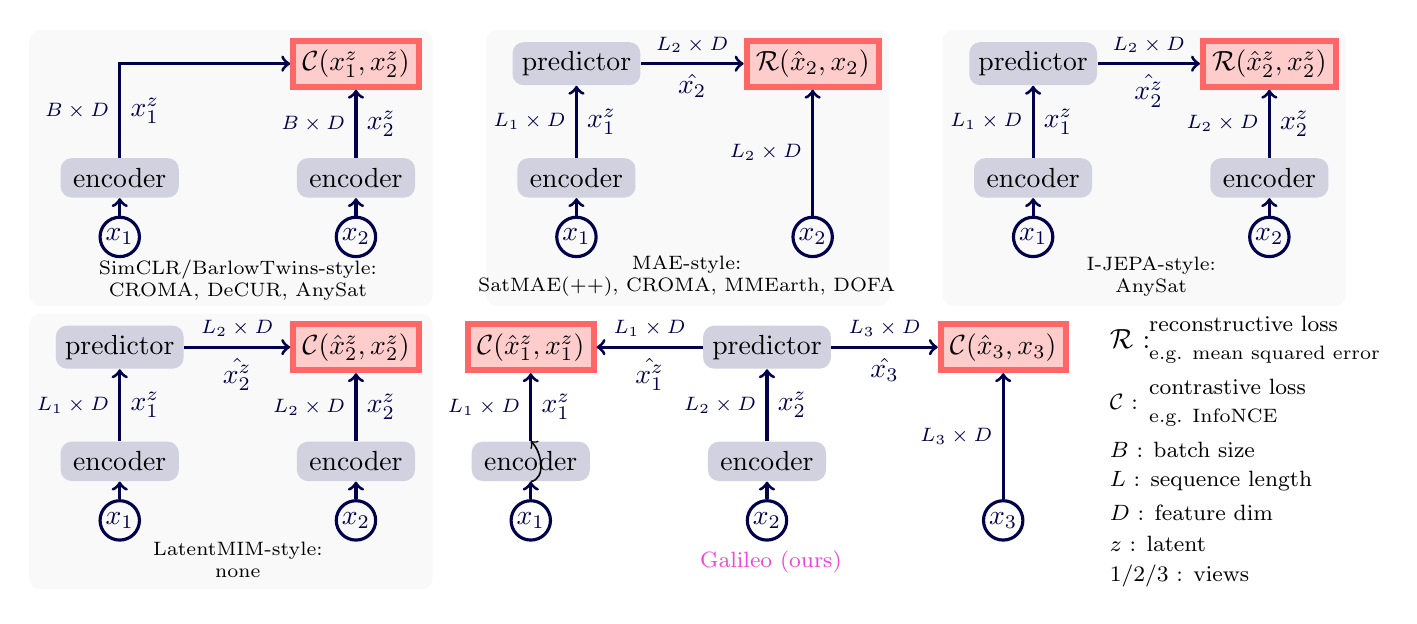
\begin{tikzpicture}
    % Define spacing variables
    \def\horizontalGap{6}     % Gap between x and y components
    \def\verticalGap{1.5}       % Gap between circles and encoders
    \def\verticalGapTwo{2.2}       % Gap between encoders and predictors
    \def\encoderWidth{1.5}    % Width of rectangles
    \def\encoderHeight{0.5}     % Height of rectangles
    \def\circleSize{0.5}        % Size of circles
    \def\lossThickness{0.75mm} % Thickness of loss rectangle border
    \def\diagramGapX{5.8}        % Gap between the two diagrams
    \def\diagramGapXBOT{6}
    \def\diagramGapY{3.6}        % Gap between the two diagrams
    \def\zOffset{2.75}           % Distance from z to predictor
    \def\linewidth{0.4mm} 
    \def\scaleMe{0.5}
    \def\spaceBetweenNotations{0.8}
    \def\inputFontSize{\normalsize}
    
    % Define custom colors
    \definecolor{encoder_bg}{HTML}{d1d1e0}
    \definecolor{loss_bg}{HTML}{ffcccc}    % Background color for loss
    \definecolor{lines}{HTML}{00004d}
    \definecolor{loss_border}{HTML}{ff6666} % Color for loss border
    \definecolor{z_color}{HTML}{ff6666}     % New color for z circle 
    \definecolor{subfigBg}{HTML}{F9F9F9}  % background color for all subfigures
    % \definecolor{GalileoBg}{HTML}{verylighthannah}
    
    % MAE
    \begin{scope}[xshift=\diagramGapX cm, scale=\scaleMe]
        % Define styles
        \fill[subfigBg, rounded corners] (-2.3,-1.75) rectangle (7.95,5.25);  % Adjust these coordinates
        \tikzstyle{circle_style} = [circle, draw, minimum size=\circleSize cm, inner sep=0pt]
        \tikzstyle{encoder_style} = [rectangle, minimum width=\encoderWidth cm, minimum height=\encoderHeight cm, rounded corners, fill=encoder_bg]
        \tikzstyle{loss_style} = [rectangle, minimum width=\encoderWidth cm, minimum height=\encoderHeight cm, draw=loss_border, line width=\lossThickness, fill=loss_bg]
        % Draw the circles at the bottom
        \node[circle_style, line width=\linewidth, color=lines, font=\inputFontSize] (circle_x) at (0, 0) {$x_1$};
        \node[circle_style, line width=\linewidth, color=lines, font=\inputFontSize] (circle_y) at (\horizontalGap, 0) {$x_2$};
        \node[encoder_style] (encoder_x) at (0, \verticalGap) {encoder};

        % Add predictor rectangle above x-encoder
        \node[encoder_style] (predictor) at (0, \verticalGapTwo * 2) {predictor};
        % Add circle to the left of predictor with custom color
        % \node[circle_style, line width=\linewidth, color=z_color, font=\LARGE] (circle_z) at (-\zOffset, \verticalGapTwo * 2) {$z$};
        % Add loss rectangle above y-encoder
        \node[loss_style] (loss) at (\horizontalGap, \verticalGapTwo * 2) {$\mathcal{R}(\hat x_2, x_2)$};

        % Draw arrows
        \draw[->, line width=\linewidth, color=lines] (circle_x.north) -- (encoder_x.south);
        \draw[->, line width=\linewidth, color=lines] (circle_y.north) -- (loss.south) node[midway, left] {\scriptsize $L_2\times D$};
        \draw[->, line width=\linewidth, color=lines] (encoder_x.north) -- (predictor.south) node[midway, left, font=\scriptsize] {$L_1\times D$}
        node[midway, right] {$x^z_1$};
        \draw[->, line width=\linewidth, color=lines] (predictor.east) -- (loss.west) node[midway, below] {$\hat{x_2}$}
        node[midway, above, font=\scriptsize] {$L_2\times D$};

        \node[font=\scriptsize, align=center] at (2.8, -1.0) {
           MAE-style:\\
           SatMAE(++), CROMA, MMEarth, DOFA
        };
        
    \end{scope}
    
    % I-JEPA
    \begin{scope}[xshift=2*\diagramGapX cm, scale=\scaleMe]
        % Define styles
        \fill[subfigBg, rounded corners] (-2.3,-1.75) rectangle (7.95,5.25);  % Adjust these coordinates
        \tikzstyle{circle_style} = [circle, draw, minimum size=\circleSize cm, inner sep=0pt]
        \tikzstyle{encoder_style} = [rectangle, minimum width=\encoderWidth cm, minimum height=\encoderHeight cm, rounded corners, fill=encoder_bg]
        \tikzstyle{loss_style} = [rectangle, minimum width=\encoderWidth cm, minimum height=\encoderHeight cm, draw=loss_border, line width=\lossThickness, fill=loss_bg]
        % Draw the circles at the bottom
        \node[circle_style, line width=\linewidth, color=lines, font=\inputFontSize] (circle_x) at (0, 0) {$x_1$};
        \node[circle_style, line width=\linewidth, color=lines, font=\inputFontSize] (circle_y) at (\horizontalGap, 0) {$x_2$};
        \node[encoder_style] (encoder_x) at (0, \verticalGap) {encoder};
        \node[encoder_style] (encoder_y) at (\horizontalGap, \verticalGap) {encoder};
        % Add predictor rectangle above x-encoder
        \node[encoder_style] (predictor) at (0, \verticalGapTwo * 2) {predictor};
        % Add circle to the left of predictor with custom color
        %\node[circle_style, line width=\linewidth, color=z_color, font=\LARGE] (circle_z) at (-\zOffset, \verticalGapTwo * 2) {$z$};
        % Add loss rectangle above y-encoder
        \node[loss_style] (loss) at (\horizontalGap, \verticalGapTwo * 2) {$\mathcal{R}(\hat x^z_2, x^z_2)$};

        % Draw arrows
        \draw[->, line width=\linewidth, color=lines] (circle_x.north) -- (encoder_x.south);
        \draw[->, line width=\linewidth, color=lines] (circle_y.north) -- (encoder_y.south);
        \draw[->, line width=\linewidth, color=lines] (encoder_y.north) -- (loss.south)
        node[midway, right] {$x^z_2$}
        node[midway, left] {\scriptsize $L_2\times D$};
        \draw[->, line width=\linewidth, color=lines] (encoder_x.north) -- (predictor.south) node[midway, left] {\scriptsize $L_1\times D$}
        node[midway, right] {$x^z_1$};
        \draw[->, line width=\linewidth, color=lines] (predictor.east) -- (loss.west) node[midway, below] {$\hat{x^z_2}$}
        node[midway, above] {\scriptsize $L_2\times D$};
        % \draw[->, line width=\linewidth, color=z_color] (circle_z.east) -- (predictor.west);

        \node[font=\scriptsize, align=center] at (3.0, -1.0) {
           I-JEPA-style:\\
           AnySat
        };
    \end{scope}

    % Sample contrastive
    \begin{scope}[scale=\scaleMe]
        % Define styles
        \fill[subfigBg, rounded corners] (-2.3,-1.75) rectangle (7.95,5.25);  % Adjust these coordinates
        \tikzstyle{circle_style} = [circle, draw, minimum size=\circleSize cm, inner sep=0pt]
        \tikzstyle{encoder_style} = [rectangle, minimum width=\encoderWidth cm, minimum height=\encoderHeight cm, rounded corners, fill=encoder_bg]
        \tikzstyle{loss_style} = [rectangle, minimum width=\encoderWidth cm, minimum height=\encoderHeight cm, draw=loss_border, line width=\lossThickness, fill=loss_bg]
        % Draw the circles at the bottom
        \node[circle_style, line width=\linewidth, color=lines, font=\inputFontSize] (circle_x) at (0, 0) {$x_1$};
        \node[circle_style, line width=\linewidth, color=lines, font=\inputFontSize] (circle_y) at (\horizontalGap, 0) {$x_2$};
        \node[encoder_style] (encoder_x) at (0, \verticalGap) {encoder};
        \node[encoder_style] (encoder_y) at (\horizontalGap, \verticalGap) {encoder};

        % Add loss rectangle above y-encoder
        \node[loss_style] (loss) at (\horizontalGap, \verticalGapTwo * 2) {$\mathcal{C}(x^z_1, x^z_2)$};

        % Draw arrows
        \draw[->, line width=\linewidth, color=lines] (circle_x.north) -- (encoder_x.south);
        \draw[->, line width=\linewidth, color=lines] (encoder_x.north) -- (encoder_x.north |- loss.west)
        node[midway, left] {\scriptsize$B\times D$}
        node[midway, right] {$x^z_1$}
        -- (loss.west);
        \draw[->, line width=\linewidth, color=lines] (circle_y.north) -- (encoder_y.south);
        \draw[->, line width=\linewidth, color=lines] (encoder_y.north) -- (loss.south)
        node[midway, right] {$x^z_2$}
        node[midway, left] {\scriptsize$B\times D$};

        % \node[font=\scriptsize] (predictor) at (2.9, -1.5) {SimCLR/BarlowTwins-style: SeCo, DeCUR};
        \node[font=\scriptsize, align=center] at (3.0, -1.1) {
           SimCLR/BarlowTwins-style:\\
           CROMA, DeCUR, AnySat
        };
    \end{scope}

    % LatentMIM
    \begin{scope}[yshift=-\diagramGapY cm, scale=\scaleMe]
        % Define styles
        \fill[subfigBg, rounded corners] (-2.3,-1.75) rectangle (7.95,5.25);  % Adjust these coordinates
        \tikzstyle{circle_style} = [circle, draw, minimum size=\circleSize cm, inner sep=0pt]
        \tikzstyle{encoder_style} = [rectangle, minimum width=\encoderWidth cm, minimum height=\encoderHeight cm, rounded corners, fill=encoder_bg]
        \tikzstyle{loss_style} = [rectangle, minimum width=\encoderWidth cm, minimum height=\encoderHeight cm, draw=loss_border, line width=\lossThickness, fill=loss_bg]
        % Draw the circles at the bottom
        \node[circle_style, line width=\linewidth, color=lines, font=\inputFontSize] (circle_x) at (0, 0) {$x_1$};
        \node[circle_style, line width=\linewidth, color=lines, font=\inputFontSize] (circle_y) at (\horizontalGap, 0) {$x_2$};
        \node[encoder_style] (encoder_x) at (0, \verticalGap) {encoder};
        \node[encoder_style] (encoder_y) at (\horizontalGap, \verticalGap) {encoder};
        % Add predictor rectangle above x-encoder
        \node[encoder_style] (predictor) at (0, \verticalGapTwo * 2) {predictor};
        % Add circle to the left of predictor with custom color
        % \node[circle_style, line width=\linewidth, color=z_color, font=\LARGE] (circle_z) at (-\zOffset, \verticalGapTwo * 2) {$z$};
        % Add loss rectangle above y-encoder
        \node[loss_style] (loss) at (\horizontalGap, \verticalGapTwo * 2) {$\mathcal{C}(\hat x^z_2, x^z_2)$};

        % Draw arrows
        \draw[->, line width=\linewidth, color=lines] (circle_x.north) -- (encoder_x.south);
        \draw[->, line width=\linewidth, color=lines] (circle_y.north) -- (encoder_y.south);
        \draw[->, line width=\linewidth, color=lines] (encoder_y.north) -- (loss.south)
        node[midway, right] {$x^z_2$}
        node[midway, left] {\scriptsize$L_2\times D$};
        \draw[->, line width=\linewidth, color=lines] (encoder_x.north) -- (predictor.south) node[midway, left] {\scriptsize$L_1\times D$}
        node[midway, right] {$x^z_1$};
        \draw[->, line width=\linewidth, color=lines] (predictor.east) -- (loss.west) node[midway, below] {$\hat{x^z_2}$}
        node[midway, above] {\scriptsize$L_2\times D$};
        % \draw[->, line width=\linewidth, color=z_color] (circle_z.east) -- (predictor.west);
        \node[font=\scriptsize, align=center] at (3.0, -1.0) {
           LatentMIM-style:\\
           none
        };
    \end{scope}

    % Galileo
    \begin{scope}[xshift=0.62*\diagramGapXBOT cm, yshift=-\diagramGapY cm, scale=\scaleMe]
        % Define styles
        % \fill[verylighthannah, rounded corners] (0.3,-1.75) rectangle (16.9,5.25);  % Adjust these coordinates
        \tikzstyle{circle_style} = [circle, draw, minimum size=\circleSize cm, inner sep=0pt]
        \tikzstyle{encoder_style} = [rectangle, minimum width=\encoderWidth cm, minimum height=\encoderHeight cm, rounded corners, fill=encoder_bg]
        \tikzstyle{loss_style} = [rectangle, minimum width=\encoderWidth cm, minimum height=\encoderHeight cm, draw=loss_border, line width=\lossThickness, fill=loss_bg]
        % Draw the circles at the bottom
        \node[circle_style, line width=\linewidth, color=lines, font=\inputFontSize] (circle_x) at (9, 0) {$x_2$};
        \node[circle_style, line width=\linewidth, color=lines, font=\inputFontSize] (circle_y) at (9 + \horizontalGap, 0) {$x_3$};
        \node[circle_style, line width=\linewidth, color=lines, font=\inputFontSize] (circle_y_left) at (9 - \horizontalGap, 0) {$x_1$};
        \node[encoder_style] (encoder_x) at (9, \verticalGap) {encoder};
        \node[encoder_style] (encoder_y) at (9 - \horizontalGap, \verticalGap) {encoder};

        % Add predictor rectangle above x-encoder
        \node[encoder_style] (predictor) at (9, \verticalGapTwo * 2) {predictor};
        % Add circle to the left of predictor with custom color
        % \node[circle_style, line width=\linewidth, color=z_color, font=\LARGE] (circle_z) at (-\zOffset, \verticalGapTwo * 2) {$z$};
        % Add loss rectangle above y-encoder
        \node[loss_style] (loss) at (9 + \horizontalGap, \verticalGapTwo * 2) {$\mathcal{C}(\hat x_3, x_3)$};
        \node[loss_style] (loss_left) at (9 - \horizontalGap, \verticalGapTwo * 2) {$\mathcal{C}(\hat x^z_1, x^z_1)$};

        % Draw arrows
        \draw[->, line width=\linewidth, color=lines] (circle_x.north) -- (encoder_x.south);
        \draw[->, line width=\linewidth, color=lines] (circle_y.north) -- (loss.south)
        node[midway, left] {\scriptsize $L_3\times D$};
        \draw[->, line width=\linewidth, color=lines] (circle_y_left.north) -- (encoder_y.south);
        \draw[->, line width=0.5*\linewidth] (encoder_y.south) to[out=10,in=-45] (encoder_y.north);

        \draw[->, line width=\linewidth, color=lines] (encoder_x.north) -- (predictor.south) node[midway, left] {\scriptsize $L_2\times D$}
        node[midway, right] {$x^z_2$};
        \draw[->, line width=\linewidth, color=lines] (predictor.east) -- (loss.west) node[midway, below] {$\hat{x_3}$}
        node[midway, above] {\scriptsize $L_3\times D$};
        \draw[->, line width=\linewidth, color=lines] (encoder_y.north) -- (loss_left.south) node[midway, right] {$x^z_1$}
        node[midway, left] {\scriptsize$L_1\times D$};
        % \draw[->, line width=\linewidth, color=z_color] (circle_z.east) -- (predictor.west);
        \draw[->, line width=\linewidth, color=lines] (predictor.west) -- (loss_left.east) node[midway, below] {$\hat{x^z_1}$} node[midway, above]{\scriptsize $L_1\times D$};

        \node[font=\footnotesize, align=center, color=ourcolor] at (9.20, -1.05) {
           Galileo (ours)
        };
    \end{scope}

    \begin{scope}[xshift=2.075*\diagramGapXBOT cm, yshift=-0.75*\diagramGapY cm, scale=\scaleMe]
        \node[anchor=west, font=\footnotesize] (text_b) at (1,4*\spaceBetweenNotations) {reconstructive loss};
        \node[anchor=west] (text_b) at (0,3.5*\spaceBetweenNotations) {$\mathcal{R}$ :};
        \node[anchor=west, font=\scriptsize] (text_b) at (1,3*\spaceBetweenNotations) {e.g. mean squared error};
    
        \node[anchor=west, font=\footnotesize] (text_b) at (1,2.0*\spaceBetweenNotations) {contrastive loss};
        \node[anchor=west, font=\footnotesize] (text_b) at (0,1.5*\spaceBetweenNotations) {$\mathcal{C}$ :};
        \node[anchor=west, font=\scriptsize] (text_b) at (1,1.0*\spaceBetweenNotations) {e.g. InfoNCE};
        
        \node[anchor=west, font=\footnotesize] (text_b) at (0,0) {$B$ : batch size};
        \node[anchor=west, font=\footnotesize] (text_l) at (0,-1*\spaceBetweenNotations) {$L$ : sequence length};
        \node[anchor=west, font=\footnotesize] (text_d) at (0,-2*\spaceBetweenNotations) {$D$ : feature dim};
        \node[anchor=west, font=\footnotesize] (text_z) at (0,-3*\spaceBetweenNotations) {$z$ : latent};
        \node[anchor=west, font=\footnotesize] (text_v) at (0,-4*\spaceBetweenNotations) {$1/2/3$ : views};
    \end{scope}
    
\end{tikzpicture}
\caption{\textbf{\emph{SSL for RS}}. \textbf{Top left:} Attracts representations originating from the same sample and repels representations from other samples. \textbf{Top center:} Predicts pixels of hidden patches. \textbf{Top right:} Predicts representations of hidden patches. \textbf{Bottom left:} Attracts representations originating from the same patch and repels representations from other patches. \textbf{Galileo (ours):} Our method simultaneously attracts varied-level representations originating from the same patch and repels elsewhere --- and attracts pixel predictions originating from the same patch and repels elsewhere. This strategy encourages learning global \emph{and} local features.}
\label{fig:system}
\end{figure*}

We address these challenges by proposing a new family of pretrained RS models called ``Galileo'' (\textbf{G}lobal \textbf{a}nd \textbf{L}ocal Flex\textbf{i}b\textbf{l}e \textbf{E}arth \textbf{O}bservation models). We develop a highly multimodal dataset that varies in space and time to train these models, and we modify the ViT architecture \cite{dosovitskiy2021an} to process this dataset. We present a novel self-supervised learning (SSL) algorithm to learn useful representations of small- and large-scale features. Our algorithm combines two training objectives: one makes predictions in (essentially) the pixel space, and the other makes predictions in the latent space (Figure \ref{fig:system}). We show that these dual objectives are complementary and necessary to improve training stability and achieve good performance across all task scales.

We demonstrate the efficacy of our Galileo models via an extensive benchmarking suite, covering many applications, domains, and RS data types. Fair comparison of RS models is challenging \cite{Corley_2024_CVPR}. To achieve this, we run hundreds of experiments across $16$ pretrained RS baselines to robustly compare with existing methods. 

% \begin{figure}[h]
    \centering
    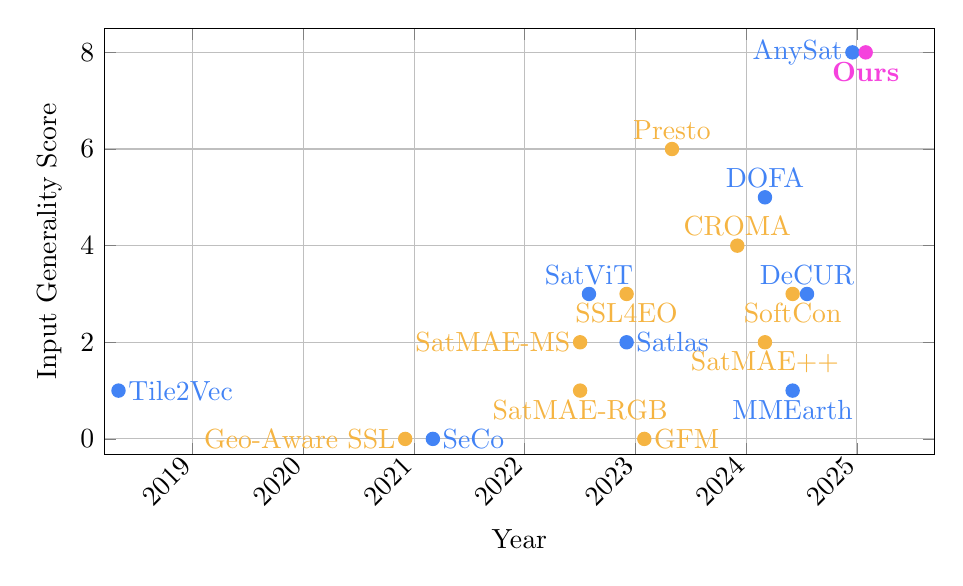
\begin{tikzpicture}
        \begin{axis}[
            width=\columnwidth,
            height=7cm,
            xmin=2018.2, xmax=2025.7, % Limits to cover the full date range
            ymin=-0.33, ymax=8.5,
            xtick={2018, 2019, 2020, 2021, 2022, 2023, 2024, 2025},
            xticklabel style={rotate=45, anchor=east, /pgf/number format/precision=0, /pgf/number format/use comma=false, /pgf/number format/1000 sep={}}, % Ensures no commas and integer formatting
            xlabel={Year},
            ylabel={Input Generality Score},
            grid=major,
        ]
            % Scatter plot points with decimal year representation
            \addplot[only marks, mark=*, mark options={scale=1.2, color=secondcolor}] coordinates {(2018.33, 1)}; % May 2018, Tile2Vec
            \addplot[only marks, mark=*, mark options={scale=1.2, color=secondcolor}] coordinates {(2021.17, 0)}; % March 2021, SeCo
            \addplot[only marks, mark=*, mark options={scale=1.2, color=thirdcolor}] coordinates {(2020.92, 0)}; % November 2020, Geo-Aware
            \addplot[only marks, mark=*, mark options={scale=1.2, color=secondcolor}] coordinates {(2022.58, 3)}; % August 2022, SatViT
            \addplot[only marks, mark=*, mark options={scale=1.2, color=thirdcolor}] coordinates {(2022.5, 1)};  % July 2022, SatMAE-RGB
            \addplot[only marks, mark=*, mark options={scale=1.2, color=thirdcolor}] coordinates {(2022.5, 2)};  % July 2022, SatMAE-MS
            \addplot[only marks, mark=*, mark options={scale=1.2, color=thirdcolor}] coordinates {(2022.92, 3)}; % November 2022, SSL4EO
            \addplot[only marks, mark=*, mark options={scale=1.2, color=secondcolor}] coordinates {(2022.92, 2)}; % November 2022, Satlas
            \addplot[only marks, mark=*, mark options={scale=1.2, color=thirdcolor}] coordinates {(2023.08, 0)}; % February 2023, GFM
            \addplot[only marks, mark=*, mark options={scale=1.2, color=thirdcolor}] coordinates {(2023.33, 6)}; % April 2023, Presto
            \addplot[only marks, mark=*, mark options={scale=1.2, color=secondcolor}] coordinates {(2024.55, 3)}; % July 2024, DeCUR
            \addplot[only marks, mark=*, mark options={scale=1.2, color=thirdcolor}] coordinates {(2023.92, 4)}; % November 2023, CROMA
            \addplot[only marks, mark=*, mark options={scale=1.2, color=thirdcolor}] coordinates {(2024.17, 2)}; % March 2024, SatMAE++
            \addplot[only marks, mark=*, mark options={scale=1.2, color=secondcolor}] coordinates {(2024.17, 5)}; % March 2024, DOFA
            \addplot[only marks, mark=*, mark options={scale=1.2, color=thirdcolor}] coordinates {(2024.42, 3)}; % May 2024, SoftCon
            \addplot[only marks, mark=*, mark options={scale=1.2, color=secondcolor}] coordinates {(2024.42, 1)}; % May 2024, MMEarth
            \addplot[only marks, mark=*, mark options={scale=1.2, color=secondcolor}] coordinates {(2024.96, 8)}; % December 2024, Anysat (ours)
            \addplot[only marks, mark=*, mark options={scale=1.2, color=ourcolor}] coordinates {(2025.08, 8)}; % January 2025, Biggie Smalls (ours)


            % Manually place labels at specified offsets
            \node[anchor=north, text=thirdcolor] at (axis cs:2022.5, 1) {SatMAE-RGB};
            \node[anchor=east, text=thirdcolor] at (axis cs:2022.5, 2) {SatMAE-MS};
            \node[anchor=north, text=thirdcolor] at (axis cs:2024.17, 2) {SatMAE++};
            \node[anchor=south, text=thirdcolor] at (axis cs:2023.92, 4) {CROMA};
            \node[anchor=north, text=thirdcolor] at (axis cs:2024.42, 3) {SoftCon};
            \node[anchor=south, text=secondcolor] at (axis cs:2024.17, 5) {DOFA};
            \node[anchor=west, text=secondcolor] at (axis cs:2022.92, 2) {Satlas};
            \node[anchor=north, text=secondcolor] at (axis cs:2024.42, 1) {MMEarth};
            \node[anchor=south, text=secondcolor] at (axis cs:2024.55, 3) {DeCUR};
            \node[anchor=south, text=thirdcolor] at (axis cs:2023.33, 6) {Presto};
            \node[anchor=west, text=thirdcolor] at (axis cs:2023.08, 0) {GFM};
            \node[anchor=north, text=ourcolor] at (axis cs:2025.08, 8) {\textbf{Ours}};
            \node[anchor=south, text=secondcolor] at (axis cs:2022.58, 3) {SatViT};
            \node[anchor=north, text=thirdcolor] at (axis cs:2022.92, 3) {SSL4EO};
            \node[anchor=east, text=thirdcolor] at (axis cs:2020.92, 0) {Geo-Aware SSL};
            \node[anchor=west, text=secondcolor] at (axis cs:2018.33, 1) {Tile2Vec};
            \node[anchor=west, text=secondcolor] at (axis cs:2021.17, 0) {SeCo};
            \node[anchor=east, text=secondcolor] at (axis cs:2024.96, 8) {AnySat};
        \end{axis}
    \end{tikzpicture}
    \caption{%
    Input Generality Score of pretrained RS models.
    One point for ingesting each of: multispectral imagery, SAR imagery, joint multispectral and SAR data, optional multispectral and SAR data, optional multispectral channel groups, $\textgreater1$ timestep, $\textgreater4$ timesteps, other RS data products.
    Colors have no meaning.}
    \label{fig:model_performance}
\end{figure}

\section{Multi-modal \& Multi-scale Self-Supervision}

\definecolor{missinggray}{gray}{0.75}
\definecolor{customgray}{gray}{0.5}
\begin{table*}[!t]
\centering \footnotesize
\caption{A comparison of model performance and model flexibility. \textbf{Performance} is measured via rankings (where lower numbers are better) on image tasks in Tables \ref{tab:knn_full}, \ref{tab:ft_full} \& \ref{tab:seg_results_full} and pixel-timeseries tasks in Table \ref{tab:ts_results}.
%, with best results \textbf{bolded} and second best results \underline{underlined}. 
For clarity, we select the best architecture per method; full rankings are available in Table \ref{tab:ranks}. 
\textbf{Flexibility} is measured by documenting which inputs are supported by the models: MultiSpectral (MS), Synthetic Aperture Radar (SAR), additional Remote Sensing modalities (+modalities), inputs with spatial dimensions and inputs with more than 1 or 4 timesteps. The Galileo models are both the best performing and the most flexible models. In particular, Galileo-Base is the best performing model when compared to both image-specialized models and pixel-timeseries specialized models.}
\label{tab:ranks_subset}
    \renewcommand{\arraystretch}{0.6}
    \begin{tabular}{
        l
        l
        c
        c
        c
        c
        c
        c
        c
        c
    }
    \toprule
    & & \multicolumn{2}{c}{Rank $\downarrow$} & \multicolumn{6}{c}{Supported Inputs} \\
     \cmidrule(lr){5-10}
        Method & Arch. & Images & \makecell{Pixel-\\timeseries} & MS & SAR & +modalities & Spatial dims & $>1$ timestep & $>4$ timesteps 
         \\
        \midrule
        % SatMAE & ViT-Base & 11.9 & {\color{missinggray} N/A} \\
        SatMAE & ViT-Large & 10.4 & {\color{missinggray} N/A} & \checkmark & & &\checkmark \\
        SatMAE++ & ViT-Large & 10.9 & {\color{missinggray} N/A} & \checkmark & & & \checkmark \\
        CROMA & ViT-Base & \underline{4.3} &  {\color{missinggray} N/A} & \checkmark & \checkmark &  & \checkmark \\
        % CROMA & ViT-Large & 4.3 & {\color{missinggray} N/A}  \\
        % SoftCon & ViT-Small & 6.3 & {\color{missinggray} N/A}  \\
        SoftCon & ViT-Base & 5.9 & {\color{missinggray} N/A} & \checkmark & \checkmark & & \checkmark \\
        % DOFA & ViT-Base & 8.9 & {\color{missinggray} N/A} \\
        DOFA & ViT-Large & 9.4 & {\color{missinggray} N/A} & \checkmark & \checkmark & & \checkmark \\
        Satlas & Swin-Tiny & 12.9 & {\color{missinggray} N/A} & \checkmark & &  &\checkmark & \checkmark \\
        % Satlas & Swin-Base & 14.5 & {\color{missinggray} N/A} \\
        MMEarth & CNN-atto & 12.3 & {\color{missinggray} N/A} & \checkmark & & & \checkmark \\
        DeCUR & ViT-Small & 8.3 & {\color{missinggray} N/A} & \checkmark & \checkmark & & \checkmark \\
        Prithvi 2.0 & ViT-Large & 11.7 & {\color{missinggray} N/A} & \checkmark & & & \checkmark & \checkmark & \\
        AnySat & ViT-Base & 11.1 & 4.5 & \checkmark & \checkmark & \checkmark & \checkmark & \checkmark & \checkmark \\
        Presto & ViT-Presto & {\color{missinggray} N/A} & 3.0 & \checkmark & \checkmark & \checkmark & & \checkmark & \checkmark \\
        \color{ourcolor}\textbf{Galileo} & ViT-Nano & 10.9 & 3.5 & \checkmark & \checkmark & \checkmark & \checkmark & \checkmark & \checkmark \\
        \color{ourcolor}\textbf{Galileo} & ViT-Tiny & 6.4 & \underline{2.3} & \checkmark & \checkmark & \checkmark & \checkmark & \checkmark & \checkmark\\
        \color{ourcolor}\textbf{Galileo} & ViT-Base & \textbf{3.0} & \textbf{1.8} & \checkmark & \checkmark & \checkmark & \checkmark & \checkmark & \checkmark \\
        \bottomrule
    \end{tabular}
\end{table*}

We aim to pretrain a model that can be applied to a range of RS tasks, even when few labels are available. This requires that we can (i) process many different modalities, (ii) ingest varying input shapes, and (iii) model phenomena that occur at very different scales. 

To train a model with capabilities for multimodal processing and input shape flexibility, we first build a pretraining dataset where each training instance includes data for multiple RS modalities, and captures data across a suitably large spatial and temporal range. During model pretraining, we subsample modalities and input shapes (subsetting space and time) from this dataset, such that the resulting model can process multi-scale and multimodal RS data. 

However, a traditional ViT architecture expects samples to share the same modalities and input shapes. We therefore adapt the ViT architecture to ingest arbitrary subsets of modalities, with varying input shapes.

Most existing SSL algorithms have been developed to be effective on natural imagery rather than RS data. We therefore develop a novel SSL algorithm that learns strong representations of both: (i) large objects and lower-frequency features, and (ii) tiny objects and high-frequency features. We achieve this by integrating two complementary algorithms, each specialized for a different scale of feature extraction.

\subsection{Achieving Flexibility via the Data and Architecture}

\subsubsection{Collecting Diverse Pretraining Data} \label{sec:dataset}

We collect a large, globally sampled pretraining dataset of \num{127155} training instances. Section \ref{app:pretraining_dataset} describes our dataset sampling process. We include a wide range of RS inputs to serve diverse applications. A training instance consists of \num{4} types of data covering \num{9} RS data modalities. We select these modalities based on their uses in past machine learning for remote sensing efforts \cite{van2023worldcereal,beukema2023satellite,poggio2021soilgrids}.

We group the modalities by whether they vary in space, time, both, or neither.
A single instance consists of $24$ monthly timesteps and $96 \times 96$ pixels at a $10$m/pixel resolution.

\textbf{Space-time varying data.} These data consist of imagery acquired by Sentinel-1 \& -2 satellites. For Sentinel-1, we take the VV and VH polarizations; and for Sentinel-2, we take all bands except the B1, B9 and B10 bands. All bands are resampled to a $10$m/pixel resolution. We also include NDVI \cite{tucker1979red} from Sentinel-2 as an input. 

\textbf{Space varying data.} These data consist of elevation and slope captured by the Shuttle Radar Topography Mission \cite{srtm}, which are constant in time; Dynamic World land cover map probabilities \cite{brown2022dynamic}, averaged over time for temporal consistency; and World Cereal agricultural land cover maps \cite{van2023worldcereal}.

\textbf{Time varying data.} These data consist of precipitation and temperature from the ERA5 dataset \cite{hersbach2020era5}; climate water deficit, soil moisture, and actual evapotranspiration from TerraClimate \cite{abatzoglou2018terraclimate}; and VIIRS nighttime lights \cite{elvidge2017viirs}. Although these modalities vary in space as well, their spatial resolution (ERA5 has a spatial resolution of tens of kilometres per pixel) means we treat them as static in space from the perspective of a single instance.

\textbf{Static data.} These data consist of population estimates from the LandScan dataset \cite{dobson2000landscan}, the spatial location of the instance, defined by its central latitude and longitude, Dynamic World classes spatially averaged over the instance, and World Cereal agricultural land cover maps spatially averaged over the instance. We include the averaged Dynamic World and World Cereal inputs in addition to the space-varying inputs. 

\subsubsection{Architecting a ViT for All Inputs}\label{sec:architecture}

We require a model for the wide range of modalities and input shapes in our dataset to handle the variety of RS data inputs (Section \ref{sec:dataset}).
Transformers are general architectures, but still require tokenization strategies to handle the varied input dimensions of space, time, and modality.

We adapt the ViT \cite{dosovitskiy2021an} architecture to ingest channel groups and \textit{variable} input shapes and timesteps, as follows:

\textbf{Patchification and Channel-group projections.} We group all inputs described in Section \ref{sec:dataset} into ``channel-groups'' when projecting the input to the encoder dimension, where a channel-group combines semantically cohesive channels (e.g. the RGB bands from Sentinel-2). We patchify --- i.e., split the input tensor into spatial squares, timesteps, and channel groups --- and project our inputs to the encoder dimension $D$ using the following transformations: (i) Space-time data, $\mathbb{R}^{H \times W \times T \times C} \rightarrow \mathbb{R}^{\frac{H}{P} \cdot \frac{W}{P} \cdot T \cdot G \times D}$, $H$ is the height, $W$ is the width, $P$ is the patch size (in pixels per side), $T$ is the timesteps, $C$ are the channels, $G$ are the channel groups. (ii) Space data, $\mathbb{R}^{H \times W \times C} \rightarrow \mathbb{R}^{\frac{H}{P} \cdot \frac{W}{P} \cdot G \times D}$, (iii) Time data, $\mathbb{R}^{T \times C} \rightarrow \mathbb{R}^{T \cdot G \times D}$, and (iv) Static data, $\mathbb{R}^{C} \rightarrow \mathbb{R}^{G \times D}$.

\textbf{Token Embeddings.} After these linear projections, our encoder creates spatial and temporal sinusoidal position embeddings, learnable channel embeddings, and month embeddings to enable seasonal reasoning; we denote these token position embeddings as $\mathtt{e} \in \mathbb{R}^{L \times D}$, where $L$ is the token sequence length. Our encoder adds these embeddings to the linear projections, previously computed. It concatenates all channel groups along the sequence dimension ---  forming our input sequence, $\mathbf{x} \in \mathbb{R}^{L \times D}$.  Importantly, our approach is robust to the presence and varying lengths of channel group sequences.

\textbf{Flexible input shapes.}

We adopt resizeable patch embeddings \cite{beyer2023flexivit}. This method resizes the weights of the ViT's linear projection layer, so that varying patch sizes $P$ can be projected into the encoder dimension. Since each token can now represent different spatial scales, we dynamically adjust the spatial positional embedding frequencies to match the spatial scale, following \citet{reed2023scale}'s ``Ground Sample Distance Positional Encodings.'': $2$D position embeddings are interpolated by a factor of $\frac{P}{H} = \frac{P}{W}$.

\subsection{Learning global and local features via SSL} \label{sec:method_ssl}

\begin{figure*}
    \centering
    %%%%%%%% 图1:  %%%%%%%%%%%%%%%%
\begin{figure}[t]
    \centering
    \includegraphics[width=\columnwidth]{Figs/01.pdf}
    \caption{Performance comparison (Top-1 Acc (\%)) under various open-vocabulary evaluation settings where the video learners except for CLIP are tuned on Kinetics-400~\cite{k400} with frozen text encoders. The satisfying in-context generalizability on UCF101~\cite{UCF101} (a) can be severely affected by static bias when evaluating on out-of-context SCUBA-UCF101~\cite{li2023mitigating} (b) by replacing the video background with other images.}
    \label{fig:teaser}
\end{figure}
    \caption{We train our model to learn both global and local features by alternating between the global (left) and local (right) pretraining tasks. These tasks differ in \circlednum{1} masking strategies and \circlednum{4} target encoding strategies. In this figure, the pretraining data is split into the channel-groups described in Section \ref{sec:architecture}.}
    \label{fig:main}
    % \vspace{-5pt}
\end{figure*}

Objects in RS data can range in size from a single pixel to hundreds or thousands of pixels. A single pretraining task is unlikely to capture this huge range in feature size, which we evidence through illustrative experiments. We introduce a novel algorithm that combines two objectives: one to learn local features and the other to learn global features. 

Our general latent prediction framework is inspired by \citet{assran2023self}, \citet{garrido2024learning}, and \citet{wei2024towards}, and operates as follows: (i) Given a batch of samples, we construct two \emph{different} views of each sample, $\mathbf{x}_1 \in \mathbb{R}^{L_1 \times D}$ and $\mathbf{x}_2 \in \mathbb{R}^{L_2 \times D}$. (ii) Our ``online'' encoder computes patch encodings $\mathbf{z}_1 = \mathbf{E}(\mathbf{x}_1)$, while our ``target'' encoder --- an exponential moving average of the online encoder --- computes target patch encodings $\mathbf{z}_2 = \mathbf{E}_{\text{EMA}}(\mathbf{x}_2)$. (iii) A predictor transformer $\mathbf{P}$ receives the target view's position, time, month, and channel group embeddings $\mathtt{e}_2 \in \mathbb{R}^{L_2 \times D}$ as placeholder queries and predicts patch encodings $\mathbf{p} \in \mathbb{R}^{L_2 \times D}$ by cross-attending to the online patch encodings, i.e., $\mathbf{p}=\mathbf{P}(\mathtt{e}_2, \mathbf{z}_1)$. (iv) The predictions $\mathbf{p}$ and targets $\mathbf{z}_2$ are compared to compute a loss $\mathcal{L}(\mathbf{p}, \mathbf{z}_2)$ that updates the online encoder. 

\subsubsection{Learning Global Features} \label{subsection:global}

Our global algorithm learns coarse-grained, lower-frequency features suited for classification applications. We modify our general latent prediction framework as follows:

\textbf{Target Depth.} Target patch encodings are typically extracted from the target view through the \textit{entire} target encoder. Some RS modalities (e.g., Dynamic World landcover classes) map closely to downstream tasks (e.g., landcover classification). These inputs may not need to be heavily processed (deeply encoded) to be useful targets. To account for the variable processing level of RS inputs, we compute targets by saving token representations after the $\ell^\text{th}$ layer, where $\ell$ varies by modality. We select $\ell$ based on each modality's abstraction level: pseudo-labels use only linear projections (no encoder layers), Sentinel-1 and Sentinel-2 use all encoder layers, and other channels use half the encoder layers. We denote our level-specific target encoder as $\mathbf{E}_{\text{EMA}}^{\ell}$.

\textbf{Loss function.} I-JEPA \cite{assran2023self} and Image World Model \cite{garrido2024learning} compute the mean-squared error (MSE) between predictions and targets. LatentMIM demonstrated superior performance via the ``Patch Discrimination'' (PatchDisc) loss \cite{wei2024towards}, which discriminates between tokens in a sample. To encourage globally discriminative representations, we extend the PatchDisc loss to better discriminate samples in a batch. We define our new loss, called AllDisc, below (note this is equivalent to PatchDisc if the $\sum_{i'}^{B}$ summation is removed):

\resizebox{!}{0.97\height}{$
    \mathcal{L}(\mathbf{u},\mathbf{v}) = \frac{-\tau}{B}\sum_{i}^{B} \frac{1}{L_i}
    \sum_{j}^{L_{i}} \log
    \frac{\text{exp}(\text{sim}(\mathbf{u}_{i,j},\mathbf{v}_{i,j})/\tau)}
    {{\sum_{i'}^{B}}
    \sum_{j'}^{L_{i'}}
    \text{exp}(\text{sim}(\mathbf{u}_{i,j},\mathbf{v}_{i',j'})/\tau)
    }
$}

with the softmax temperature $\tau$, the sample index $i$, the batch size $B$, the token index $j$, the number of tokens in the $i^{th}$ sample $L_{i}$, and the $l_2$ normalized dot product sim$(\mathbf{u},\mathbf{v}) = \mathbf{u}^{\top}\mathbf{v}/\norm{\mathbf{u}}\norm{\mathbf{v}}$. Our global loss is:

\makebox[\columnwidth]{
$\mathcal{L}_{global} = \text{AllDisc}(\mathbf{P}(\mathtt{e}_2, \mathbf{E}(\mathbf{x}_1)),\text{sg}(\mathbf{E}_{\text{EMA}}^{\ell}(\mathbf{x}_2)))$
}

where sg is the stop-gradient operation.

\textbf{Masking Strategy.} Structured or contiguous masking increases the distance between online and target tokens. This reduces the ability for the online encoder and predictor to locally interpolate between online (``visible'') tokens to predict the target token's representation. ``Space masking'' samples masks across space while maintaining consistency across channel groups and time; ``time masking'' does the same across time while maintaining consistency across channel groups and space. We alternate between the two during pretraining (see complete masking details in Appendix \ref{app:global}).

\subsubsection{Learning Local Features} \label{subsection:local}

Our local algorithm learns fine-grained, higher-frequency features suited for segmentation applications. We modify our general latent prediction framework as follows:

\textbf{Target Depth.} All prior latent prediction methods target patch representations, rather than pixels, to encourage the encoder to ignore ``low-level'' image details. While pixel-level details are usually irrelevant in natural imagery, individual pixels can contain essential details in RS. Therefore, we target the lowest representation level: the pixel space. To achieve this with a contrastive objective, we compute targets using the target encoder's linear projection, $\mathbf{E}_{\text{EMA}}^{proj}$, \emph{skipping all transformer blocks}.

\textbf{Loss Function.} MAE \cite{he2022masked} computes the MSE between predicted and hidden pixels. Although this encourages local features, we can do better by \emph{amplifying local details} via the PatchDisc loss. This combination amounts to performing contrastive learning in the pixel space; to our knowledge, ours is the first SSL algorithm to perform contrastive learning in the pixel space.

\makebox[\columnwidth]{
$\mathcal{L}_{local} = \text{PatchDisc}(\mathbf{P}(\mathtt{e}_2, \mathbf{E}(\mathbf{x}_1)), \text{sg}(\mathbf{E}_{\text{EMA}}^{proj}(\mathbf{x}_2)))$
}

\textbf{Masking Strategy.} Unstructured masking distributes the set of online and target tokens across all axes. As a result, target tokens are located close to online tokens more frequently than if contiguous masking were used. This makes local token relationships more useful to solve the pretext task. See complete masking details in Appendix \ref{app:local}.

\subsubsection{Combining Local and Global Objectives} \label{sec:combined}

While we can learn strong local and global representations independently, we aim to learn representations that excel at both. In Section \ref{sec:ablations}, we show that these goals conflict when using a single pretraining task. Better classification hurts segmentation; better segmentation hurts classification. Combining both pretraining objectives resolves this conflict.

This combination has a secondary benefit. Latent prediction frameworks are known to be unstable; they can find trivial solutions that learn useless representations. In Section \ref{sec:ablations}, we show that our dual objective algorithm is far more robust than single objectives. 

Our dual algorithm, Galileo, alternates between global and local objectives during pretraining (Figure \ref{fig:main}):

\makebox[\columnwidth]{
$\mathcal{L}_{Galileo} = \frac{1}{2}(\mathcal{L}_{global} + \mathcal{L}_{local})$
}

Ablation experiments in Section \ref{sec:ablations} show that PatchDisc outperforms AllDisc when combining global and local objectives, so we use PatchDisc for both objectives. 

\begin{table}
    \vspace{-6pt}
    \centering
    \scriptsize
    \caption{Within- and between-sample token representation similarity. Measured using the cosine similarity over all EuroSat training samples.}
    \label{tab:cosines}
    \setlength{\tabcolsep}{4pt}
    \renewcommand{\arraystretch}{1.2}
    \begin{tabular}{lcc}
        \makecell{Pretraining \\ Objective} & \makecell{Within-sample \\ Similarity} & \makecell{Between-sample \\ Similarity} \\
        \toprule
        Global only (\textsection \ref{subsection:global}) & 0.90 & 0.75 \\
        Local only (\textsection \ref{subsection:local}) & 0.66 & 0.86 \\
        Combined (\textsection \ref{sec:combined}) & 0.65 & 0.81 \\
    \end{tabular}
    \vspace{-15pt}
\end{table}


\textbf{Representation measurements.} We performed an experiment to verify our intuition about global and local algorithms. For all EuroSat training samples, we compute the cosine similarity between the token representations in a sample and then average across all samples, measuring the within-sample representational differences. Similarly, we average all tokens over each sample and then compute the cosine similarities between samples, measuring the between-sample differences. We find our local objective amplifies within-sample features, whereas our global objective amplifies between-sample features (Table \ref{tab:cosines}). We also confirm these intuitions via downstream tasks in Section \ref{sec:ablations}.

\section{Experimental Framework}

\textbf{Pretraining.} We pretrain three model sizes for $500$ epochs using the algorithm described in Section \ref{sec:combined}. Please see the Appendix for complete details.

\textbf{Downstream Tasks.}\label{section:downstream_tasks} We evaluate our model on all Sentinel-2 tasks in GeoBench \cite{lacoste2024geo}.
These cover single-timestep image classification and segmentation in various applications and geographies.
We also test on fine-grained segmentation via the MADOS marine debris dataset \cite{kikaki2024detecting}, Sentinel-1 image segmentation via Sen1Floods11 \cite{bonafilia2020sen1floods11}, image-timeseries segmentation via PASTIS \cite{garnot2021panoptic}, optical pixel-timeseries classification via Breizhcrops \cite{russwurm2019breizhcrops}, and multimodal pixel-timeseries classification via CropHarvest \cite{tseng2021cropharvest}.

\textbf{Comparisons.} \label{section:comparisons} We benchmark our models against all SOTA pretrained RS models (described in Section \ref{sec:pretrained_rs}).
We report results on the full test set for each task.
Feature scaling, image sizes, and hyperparameter selections have significant effects on model performance \cite{Corley_2024_CVPR}.
We therefore rerun evaluations for all baseline models and sweep feature scaling methods and learning rates (where appropriate).
In addition, we resize all images to the pretraining image size.
For the image classification and segmentation tasks, we measure model results across four training set sizes (``partitions''): $100$\%, $20$\%, $5$\%, and $1$\%.
We use a patch size of \num{4} for all models with variable patch sizes.
When applying single-timestep models to the multi-timestep PASTIS dataset, we additionally sweep pooling methods to pool per-timestep encodings.
See Appendix \ref{app:eval_details} for complete details.

\begin{table*}[!t]
    \newcommand{\BEST}[1]{\textbf{#1}}
    \newcommand{\SECOND}[1]{\underline{#1}}
    \newcommand{\COLUMNvalues}[2]{
        \def\COLUMNmin{#1}
        \def\COLUMNmax{#2}
        % Reset tracking for this column
        \global\def\COLUMNbest{0}
        \global\def\COLUMNsecond{0}
        \global\def\COLUMNbestrows{}
        \global\def\COLUMNsecondrows{}  % Changed to store multiple second-best rows
    }
    \newcommand{\CELLvalue}[3]{
        \ifstrequal{#3}{}
            {
                \csxdef{C#1R#2}{--}
            }{
            % Store the raw value first
            \csxdef{C#1R#2}{#3}
    
            % Update best/second best
            \ifdim #3pt > \COLUMNbest pt
                % Current value is new best
                \xdef\COLUMNsecond{\COLUMNbest}
                \xdef\COLUMNsecondrows{\COLUMNbestrows}  % Old best becomes second
                \xdef\COLUMNbest{#3}
                \xdef\COLUMNbestrows{#2}
            \else
                \ifdim #3pt = \COLUMNbest pt
                    % Tie for best
                    \xdef\COLUMNbestrows{\COLUMNbestrows,#2}
                \else
                    \ifdim #3pt = \COLUMNsecond pt
                        % Tie for second best
                        \xdef\COLUMNsecondrows{\COLUMNsecondrows,#2}
                    \else
                        \ifdim #3pt > \COLUMNsecond pt
                            % New second best
                            \xdef\COLUMNsecond{#3}
                            \xdef\COLUMNsecondrows{#2}
                        \fi
                    \fi
                \fi
            \fi
    
            % If this is the last row in the column, format all values
            \ifnum#2=18
                % Handle best values
                \foreach \bestrow in \COLUMNbestrows {
                    \csxdef{C#1R\bestrow}{\noexpand\BEST{\csuse{C#1R\bestrow}}}
                }
                % Handle second best values
                \foreach \secondrow in \COLUMNsecondrows {
                    \csxdef{C#1R\secondrow}{\noexpand\SECOND{\csuse{C#1R\secondrow}}}
                }
            \fi
            }
    }
    % Column 1
        \COLUMNvalues{82.2}{93}
        \CELLvalue{1}{1}{84.1}
        \CELLvalue{1}{2}{84.3}
        \CELLvalue{1}{3}{82.7}
        \CELLvalue{1}{4}{85.6}
        \CELLvalue{1}{5}{86.3}
        \CELLvalue{1}{6}{89.8}
        \CELLvalue{1}{7}{90.3}
        \CELLvalue{1}{8}{82.8}
        \CELLvalue{1}{9}{83.6}
        \CELLvalue{1}{10}{81.7}
        \CELLvalue{1}{11}{81.5}
        \CELLvalue{1}{12}{81.7}
        \CELLvalue{1}{13}{89.0}
        \CELLvalue{1}{14}{80.2}
        \CELLvalue{1}{15}{82.2}
        \CELLvalue{1}{16}{89.7}
        \CELLvalue{1}{17}{90.1}
        \CELLvalue{1}{18}{93.0}
        
    % Column 2
        \COLUMNvalues{69.1}{88.5}
        \CELLvalue{2}{1}{73.3}
        \CELLvalue{2}{2}{74.7}
        \CELLvalue{2}{3}{75.9}
        \CELLvalue{2}{4}{79.4}
        \CELLvalue{2}{5}{78.1}
        \CELLvalue{2}{6}{83.4}
        \CELLvalue{2}{7}{82.1}
        \CELLvalue{2}{8}{72.1}
        \CELLvalue{2}{9}{72.1}
        \CELLvalue{2}{10}{70.3}
        \CELLvalue{2}{11}{69.1}
        \CELLvalue{2}{12}{73.5}
        \CELLvalue{2}{13}{85.3}
         \CELLvalue{2}{14}{69.4}
        \CELLvalue{2}{15}{73.7}
        \CELLvalue{2}{16}{82.4}
        \CELLvalue{2}{17}{83.9}
        \CELLvalue{2}{18}{88.5}
        

    % Column 3
        \COLUMNvalues{42.1}{72.3}
        \CELLvalue{3}{1}{50.1}
        \CELLvalue{3}{2}{53.1}
        \CELLvalue{3}{3}{51.1}
        \CELLvalue{3}{4}{66.2}
        \CELLvalue{3}{5}{59.9}
        \CELLvalue{3}{6}{55.9}
        \CELLvalue{3}{7}{54.2}
        \CELLvalue{3}{8}{60.9}
        \CELLvalue{3}{9}{53.5}
        \CELLvalue{3}{10}{48.3}
        \CELLvalue{3}{11}{42.1}
        \CELLvalue{3}{12}{60.3}
        \CELLvalue{3}{13}{72.3}
        \CELLvalue{3}{14}{54.1}
        \CELLvalue{3}{15}{62.5}
        \CELLvalue{3}{16}{56.6}
        \CELLvalue{3}{17}{59.5}
        \CELLvalue{3}{18}{71.3}

    % Column 4
        \COLUMNvalues{10.0}{56.6}
        \CELLvalue{4}{1}{34.8}
        \CELLvalue{4}{2}{46.4}
        \CELLvalue{4}{3}{48.5}
        \CELLvalue{4}{4}{51.3}
        \CELLvalue{4}{5}{49.0}
        \CELLvalue{4}{6}{27.2}
        \CELLvalue{4}{7}{19.8}
        \CELLvalue{4}{8}{49.6}
        \CELLvalue{4}{9}{41.7}
        \CELLvalue{4}{10}{35.8}
        \CELLvalue{4}{11}{10.0}
        \CELLvalue{4}{12}{30.0}
        \CELLvalue{4}{13}{46.6}
        \CELLvalue{4}{14}{48.0}
        \CELLvalue{4}{15}{47.1}
        \CELLvalue{4}{16}{41.7}
        \CELLvalue{4}{17}{41.3}
        \CELLvalue{4}{18}{56.6}
        
        
    % Column 5
        \COLUMNvalues{47.0}{64.7}
        \CELLvalue{5}{1}{50.6}
        \CELLvalue{5}{2}{50.8}
        \CELLvalue{5}{3}{50.8}
        \CELLvalue{5}{4}{58.8}
        \CELLvalue{5}{5}{56.6}
        \CELLvalue{5}{6}{64.7}
        \CELLvalue{5}{7}{63.7}
        \CELLvalue{5}{8}{49.4}
        \CELLvalue{5}{9}{49.9}
        \CELLvalue{5}{10}{51.9}
        \CELLvalue{5}{11}{47.0}
        \CELLvalue{5}{12}{58.3}
        \CELLvalue{5}{13}{63.8}
        \CELLvalue{5}{14}{49.4}
        \CELLvalue{5}{15}{54.9}
        \CELLvalue{5}{16}{53.8}
        \CELLvalue{5}{17}{55.5}
        \CELLvalue{5}{18}{59.0}
        
        
    % Column 6
        \COLUMNvalues{41.1}{59.2}
        \CELLvalue{6}{1}{42.5}
        \CELLvalue{6}{2}{42.9}
        \CELLvalue{6}{3}{42.8}
        \CELLvalue{6}{4}{55.3}
        \CELLvalue{6}{5}{50.6}
        \CELLvalue{6}{6}{58.7}
        \CELLvalue{6}{7}{57.5}
        \CELLvalue{6}{8}{43.6}
        \CELLvalue{6}{9}{41.6}
        \CELLvalue{6}{10}{44.8}
        \CELLvalue{6}{11}{41.1}
        \CELLvalue{6}{12}{52.2}
        \CELLvalue{6}{13}{59.2}
        \CELLvalue{6}{14}{42.9}
        \CELLvalue{6}{15}{47.2}
        \CELLvalue{6}{16}{46.3}
        \CELLvalue{6}{17}{48.2}
        \CELLvalue{6}{18}{51.5}
        

    % Column 7
        \COLUMNvalues{35.0}{55.4}
        \CELLvalue{7}{1}{35.7}
        \CELLvalue{7}{2}{35.6}
        \CELLvalue{7}{3}{36.7}
        \CELLvalue{7}{4}{49.3}
        \CELLvalue{7}{5}{44.1}
        \CELLvalue{7}{6}{52.6}
        \CELLvalue{7}{7}{52.0}
        \CELLvalue{7}{8}{37.2}
        \CELLvalue{7}{9}{35.3}
        \CELLvalue{7}{10}{37.8}
        \CELLvalue{7}{11}{35.0}
        \CELLvalue{7}{12}{46.5}
        \CELLvalue{7}{13}{55.4}
        \CELLvalue{7}{14}{35.5}
        \CELLvalue{7}{15}{40.7}
        \CELLvalue{7}{16}{41.5}
        \CELLvalue{7}{17}{41.6}
        \CELLvalue{7}{18}{45.4}
        
        
    % Column 8
        \COLUMNvalues{25.8}{49.6}
        \CELLvalue{8}{1}{29.0}
        \CELLvalue{8}{2}{27.7}
        \CELLvalue{8}{3}{31.6}
        \CELLvalue{8}{4}{44.7}
        \CELLvalue{8}{5}{38.0}
        \CELLvalue{8}{6}{43.3}
        \CELLvalue{8}{7}{42.5}
        \CELLvalue{8}{8}{29.9}
        \CELLvalue{8}{9}{27.6}
        \CELLvalue{8}{10}{29.6}
        \CELLvalue{8}{11}{25.8}
        \CELLvalue{8}{12}{39.6}
        \CELLvalue{8}{13}{49.6}
        \CELLvalue{8}{14}{28.8}
        \CELLvalue{8}{15}{33.7}
        \CELLvalue{8}{16}{33.9}
        \CELLvalue{8}{17}{34.4}
        \CELLvalue{8}{18}{36.5}
        

    % Column 9
        \COLUMNvalues{35.6}{54.8}
        \CELLvalue{9}{1}{36.0}
        \CELLvalue{9}{2}{36.6}
        \CELLvalue{9}{3}{34.7}
        \CELLvalue{9}{4}{48.8}
        \CELLvalue{9}{5}{47.6}
        \CELLvalue{9}{6}{51.1}
        \CELLvalue{9}{7}{51.0}
        \CELLvalue{9}{8}{41.4}
        \CELLvalue{9}{9}{45.4}
        \CELLvalue{9}{10}{36.6}
        \CELLvalue{9}{11}{35.8}
        \CELLvalue{9}{12}{39.8}
        \CELLvalue{9}{13}{45.8}
        \CELLvalue{9}{14}{29.5}
        \CELLvalue{9}{15}{39.8}
        \CELLvalue{9}{16}{50.1}
        \CELLvalue{9}{17}{49.7}
        \CELLvalue{9}{18}{54.8}
        
        
    % Column 10
        \COLUMNvalues{30.7}{53.8}
        \CELLvalue{10}{1}{32.9}
        \CELLvalue{10}{2}{34.3}
        \CELLvalue{10}{3}{32.7}
        \CELLvalue{10}{4}{48.0}
        \CELLvalue{10}{5}{45.0}
        \CELLvalue{10}{6}{49.9}
        \CELLvalue{10}{7}{49.7}
        \CELLvalue{10}{8}{40.7}
        \CELLvalue{10}{9}{40.6}
        \CELLvalue{10}{10}{30.7}
        \CELLvalue{10}{11}{33.4}
        \CELLvalue{10}{12}{38.8}
        \CELLvalue{10}{13}{43.1}
        \CELLvalue{10}{14}{31.2}
        \CELLvalue{10}{15}{34.9}
        \CELLvalue{10}{16}{50.3}
        \CELLvalue{10}{17}{50.5}
        \CELLvalue{10}{18}{53.8}
        

    % Column 11
        \COLUMNvalues{29.5}{51.1}
        \CELLvalue{11}{1}{29.7}
        \CELLvalue{11}{2}{31.0}
        \CELLvalue{11}{3}{29.9}
        \CELLvalue{11}{4}{43.9}
        \CELLvalue{11}{5}{43.2}
        \CELLvalue{11}{6}{43.3}
        \CELLvalue{11}{7}{45.3}
        \CELLvalue{11}{8}{37.5}
        \CELLvalue{11}{9}{35.6}
        \CELLvalue{11}{10}{29.6}
        \CELLvalue{11}{11}{29.6}
        \CELLvalue{11}{12}{36.8}
        \CELLvalue{11}{13}{38.5}
        \CELLvalue{11}{14}{29.6}
        \CELLvalue{11}{15}{32.0}
        \CELLvalue{11}{16}{47.5}
        \CELLvalue{11}{17}{44.2}
        \CELLvalue{11}{18}{51.1}
        
    % Column 12
        \COLUMNvalues{22.7}{43.2}
        \CELLvalue{12}{1}{23.1}
        \CELLvalue{12}{2}{24.4}
        \CELLvalue{12}{3}{23.4}
        \CELLvalue{12}{4}{33.8}
        \CELLvalue{12}{5}{33.7}
        \CELLvalue{12}{6}{31.4}
        \CELLvalue{12}{7}{35.4}
        \CELLvalue{12}{8}{29.4}
        \CELLvalue{12}{9}{31.8}
        \CELLvalue{12}{10}{27.1}
        \CELLvalue{12}{11}{30.4}
        \CELLvalue{12}{12}{25.1}
        \CELLvalue{12}{13}{30.9}
        \CELLvalue{12}{14}{26.1}
        \CELLvalue{12}{15}{29.0}
        \CELLvalue{12}{16}{37.4}
        \CELLvalue{12}{17}{36.2}
        \CELLvalue{12}{18}{43.2}
        
    % Column 13
        \COLUMNvalues{80}{92.6}
        \CELLvalue{13}{1}{86.1}
        \CELLvalue{13}{2}{87.9}
        \CELLvalue{13}{3}{89.6}
        \CELLvalue{13}{4}{92.6}
        \CELLvalue{13}{5}{91.0}
        \CELLvalue{13}{6}{89.2}
        \CELLvalue{13}{7}{90.0}
        \CELLvalue{13}{8}{88.3}
        \CELLvalue{13}{9}{86.8}
        \CELLvalue{13}{10}{88.2}
        \CELLvalue{13}{11}{80.0}
        \CELLvalue{13}{12}{89.4}
        \CELLvalue{13}{13}{83.7}
        \CELLvalue{13}{14}{87.9}
        \CELLvalue{13}{15}{85.3}
        \CELLvalue{13}{16}{86.7}
        \CELLvalue{13}{17}{86.9}
        \CELLvalue{13}{18}{90.7}
        

    % Column 14
        \COLUMNvalues{78.3}{90.6}
        \CELLvalue{14}{1}{81.9}
        \CELLvalue{14}{2}{84.0}
        \CELLvalue{14}{3}{87.1}
        \CELLvalue{14}{4}{90.6}
        \CELLvalue{14}{5}{86.7}
        \CELLvalue{14}{6}{86.9}
        \CELLvalue{14}{7}{86.1}
        \CELLvalue{14}{8}{86.2}
        \CELLvalue{14}{9}{85.2}
        \CELLvalue{14}{10}{85.2}
        \CELLvalue{14}{11}{78.3}
        \CELLvalue{14}{12}{85.4}
        \CELLvalue{14}{13}{81.7}
        \CELLvalue{14}{14}{86.8}
        \CELLvalue{14}{15}{81.7}
        \CELLvalue{14}{16}{82.2}
        \CELLvalue{14}{17}{83.7}
        \CELLvalue{14}{18}{86.9}
        

    % Column 15
        \COLUMNvalues{76.9}{88.6}
        \CELLvalue{15}{1}{80.3}
        \CELLvalue{15}{2}{80.4}
        \CELLvalue{15}{3}{82.8}
        \CELLvalue{15}{4}{87.7}
        \CELLvalue{15}{5}{82.9}
        \CELLvalue{15}{6}{80.5}
        \CELLvalue{15}{7}{80.6}
        \CELLvalue{15}{8}{82.0}
        \CELLvalue{15}{9}{84.8}
        \CELLvalue{15}{10}{82.4}
        \CELLvalue{15}{11}{76.9}
        \CELLvalue{15}{12}{84.1}
        \CELLvalue{15}{13}{77.9}
        \CELLvalue{15}{14}{83.3}
        \CELLvalue{15}{15}{78.0}
        \CELLvalue{15}{16}{83.2}
        \CELLvalue{15}{17}{83.8}
        \CELLvalue{15}{18}{85.8}
        

    % Column 16
        \COLUMNvalues{73.0}{84.8}
        \CELLvalue{16}{1}{73.5}
        \CELLvalue{16}{2}{74.7}
        \CELLvalue{16}{3}{76.7}
        \CELLvalue{16}{4}{85.1}
        \CELLvalue{16}{5}{80.2}
        \CELLvalue{16}{6}{77.8}
        \CELLvalue{16}{7}{74.5}
        \CELLvalue{16}{8}{78.3}
        \CELLvalue{16}{9}{80.6}
        \CELLvalue{16}{10}{73.0}
        \CELLvalue{16}{11}{73.3}
        \CELLvalue{16}{12}{79.7}
        \CELLvalue{16}{13}{74.2}
        \CELLvalue{16}{14}{80.6}
        \CELLvalue{16}{15}{72.0}
        \CELLvalue{16}{16}{79.7}
        \CELLvalue{16}{17}{77.3}
        \CELLvalue{16}{18}{78.0}
        
    \newcommand{\CELLvaluedsaddasdsadasdad}[3]{%
        %\cellcolor{COLMAX!0!COLMED!100!COLMIN}#1
        \FPeval\MIDvalue{(#1+#2)/2}%
        \FPeval\NORMvalue{(#3-#1)*((100)/(#2-#1))}%
        #3
    }
    %
    \begin{minipage}{0.58\linewidth}
    \centering\footnotesize
    \setlength{\tabcolsep}{2pt}
    \resizebox{\textwidth}{!}{\begin{tabular}{
        l
        l
        c%S[table-format=2.2]%1
        c%S[table-format=2.2]%2
        c%S[table-format=2.2]%3
        c%S[table-format=2.2]%4
        c%S[table-format=2.2]%5
        c%S[table-format=2.2]%6
        c%S[table-format=2.2]%7
        c%S[table-format=2.2]%8
        c%S[table-format=2.2]%9
        c%S[table-format=2.2]%10
    }
         & & \multicolumn{2}{c}{\textbf{m-EuroSat}} & \multicolumn{2}{c}{\textbf{m-BigEarthNet}} & \multicolumn{2}{c}{\textbf{m-So2Sat}} & \multicolumn{2}{c}{\textbf{m-Brick-Kiln}}  \\
         & & \multicolumn{2}{c}{Training \%} & \multicolumn{2}{c}{Training \%} & \multicolumn{2}{c}{Training \%} & \multicolumn{2}{c}{Training \%}  \\
          % & & \multicolumn{2}{c}{Top-1 Acc.} & \multicolumn{2}{c}{F1 Score} & \multicolumn{2}{c}{Top-1 Acc.} & \multicolumn{2}{c}{Top-1 Acc.}  &  \\
        \cmidrule(lr){3-4}
        \cmidrule(lr){5-6}
        \cmidrule(lr){7-8}
        \cmidrule(lr){9-10}

        Method & Arch.              & 
        \multicolumn{1}{>{\centering\arraybackslash}p{21.2pt}}{$100\%$} & 
        \multicolumn{1}{>{\centering\arraybackslash}p{21.2pt}}{$1\%$} & 
        \multicolumn{1}{>{\centering\arraybackslash}p{21.2pt}}{$100\%$} & 
        \multicolumn{1}{>{\centering\arraybackslash}p{21.2pt}}{$1\%$} & 
        \multicolumn{1}{>{\centering\arraybackslash}p{21.2pt}}{$100\%$} & 
        \multicolumn{1}{>{\centering\arraybackslash}p{21.2pt}}{$1\%$} & 
        \multicolumn{1}{>{\centering\arraybackslash}p{21.2pt}}{$100\%$} & 
        \multicolumn{1}{>{\centering\arraybackslash}p{21.2pt}}{$1\%$} \\
        \toprule
        SatMAE & ViT-Base & \csuse{C1R1}  & \csuse{C4R1}  & \csuse{C5R1} & \csuse{C8R1}  & \csuse{C9R1}  &  \csuse{C12R1} & \csuse{C13R1}& \csuse{C16R1} \\
        % SatMAE \cite{cong2022satmae} & ViT-Large & \csuse{C1R2}  & \csuse{C4R2}  & \csuse{C5R2} & \csuse{C8R2}  & \csuse{C9R2}  &  \csuse{C12R2} & \csuse{C15R2}& \csuse{C16R2} \\
        SatMAE++ & ViT-Large & \csuse{C1R3}  & \csuse{C4R3}  & \csuse{C5R3} & \csuse{C8R3}  & \csuse{C9R3}  &  \csuse{C12R3} & \csuse{C13R3}& \csuse{C16R3} \\
        CROMA & ViT-Base & \csuse{C1R4}  & \csuse{C4R4}  & \csuse{C5R4} & \csuse{C8R4}  & \csuse{C9R4}  &  \csuse{C12R4} & \csuse{C13R4}& \csuse{C16R4} \\ 
        % CROMA \cite{fuller2024croma} & ViT-Large & \csuse{C1R5}  & \csuse{C4R5}  & \csuse{C5R5} & \csuse{C8R5}  & \csuse{C9R5}  &  \csuse{C12R5} & \csuse{C15R5}& \csuse{C16R5} \\
        SoftCon & ViT-Small & \csuse{C1R6}  & \csuse{C4R6}  & \csuse{C5R6} & \csuse{C8R6}  & \csuse{C9R6}  &  \csuse{C12R6} & \csuse{C13R6}& \csuse{C16R6} \\
        % SoftCon \cite{wang2024multi} & ViT-Base & \csuse{C1R7}  & \csuse{C4R7}  & \csuse{C5R7} & \csuse{C8R7}  & \csuse{C9R7}  &  \csuse{C12R7} & \csuse{C15R7}& \csuse{C16R7} \\
        DOFA & ViT-Base & \csuse{C1R8}  & \csuse{C4R8}  & \csuse{C5R8} & \csuse{C8R8}  & \csuse{C9R8}  &  \csuse{C12R8} & \csuse{C13R8}& \csuse{C16R8} \\
        % DOFA \cite{xiong2024neural} & ViT-Large & \csuse{C1R9}  & \csuse{C4R9}  & \csuse{C5R9} & \csuse{C8R9}  & \csuse{C9R9}  &  \csuse{C12R9} & \csuse{C15R9}& \csuse{C16R9} \\
        Satlas & Swin-Tiny & \csuse{C1R10}  & \csuse{C4R10}  & \csuse{C5R10} & \csuse{C8R10}  & \csuse{C9R10}  &  \csuse{C12R10} & \csuse{C13R10}& \csuse{C16R10} \\
        % Satlas \cite{bastani2023satlaspretrain} & Swin-Base & \csuse{C1R11}  & \csuse{C4R11}  & \csuse{C5R11} & \csuse{C8R11}  & \csuse{C9R11}  &  \csuse{C12R11} & \csuse{C15R11}& \csuse{C16R11}\\
        MMEarth & CNN-atto & \csuse{C1R12}  & \csuse{C4R12}  & \csuse{C5R12} & \csuse{C8R12}  & \csuse{C9R12}  &  \csuse{C12R12} & \csuse{C13R12}& \csuse{C16R12} \\
        DeCUR & ViT-Small & \csuse{C1R13}  & \csuse{C4R13}  & \csuse{C5R13} & \csuse{C8R13}  & \csuse{C9R13}  &  \csuse{C12R13} & \csuse{C13R13}& \csuse{C16R13} \\
        Prithvi 2.0 & ViT-Large & \csuse{C1R14}  & \csuse{C4R14}  & \csuse{C5R14} & \csuse{C8R14}  & \csuse{C9R14}  &  \csuse{C12R14} & \csuse{C13R14}& \csuse{C16R14} \\
        AnySat & ViT-Base & \csuse{C1R15}  & \csuse{C4R15}  & \csuse{C5R15} & \csuse{C8R15}  & \csuse{C9R15}  &  \csuse{C12R15} & \csuse{C13R15}& \csuse{C16R15} \\
        \midrule 
        \color{ourcolor}\textbf{Galileo} & ViT-Nano & \csuse{C1R16}  & \csuse{C4R16}  & \csuse{C5R16} & \csuse{C8R16}  & \csuse{C9R16}  &  \csuse{C12R16} & \csuse{C13R16}& \csuse{C16R16} \\
        \color{ourcolor}\textbf{Galileo} & ViT-Tiny & \csuse{C1R17}  & \csuse{C4R17}  & \csuse{C5R17} & \csuse{C8R17}  & \csuse{C9R17}  &  \csuse{C12R17} & \csuse{C13R17}& \csuse{C16R17} \\
        \color{ourcolor}\textbf{Galileo} & ViT-Base & \csuse{C1R18}  & \csuse{C4R18}  & \csuse{C5R18} & \csuse{C8R18}  & \csuse{C9R18}  &  \csuse{C12R18} & \csuse{C13R18}& \csuse{C16R18} \\
        % \bottomrule
    \end{tabular}}
    \end{minipage}
    \hfill
    \begin{minipage}{0.32\linewidth}
    \captionof{table}{Image classification test performance ($\%$) via $k$NN. We report Top-1 accuracies for all tasks except the multilabel BigEarthNet task (for which we report F1-score). For clarity, we select the best performing model variant per baseline method, measured across all classification tasks and partitions. These model variants in some cases differ from the model variants in Table \ref{tab:ft_subset}. Full results are available in Table \ref{tab:knn_full}. The the best and second best results in Table \ref{tab:knn_full} are \textbf{bolded} and \underline{underlined} respectively.}\label{tab:knn_subset}
    \end{minipage}
\end{table*}

\begin{table*}[!t]
    \newcommand{\BEST}[1]{\textbf{#1}}
    \newcommand{\SECOND}[1]{\underline{#1}}
    \newcommand{\COLUMNvalues}[2]{
        \def\COLUMNmin{#1}
        \def\COLUMNmax{#2}
        % Reset tracking for this column
        \global\def\COLUMNbest{0}
        \global\def\COLUMNsecond{0}
        \global\def\COLUMNbestrows{}
        \global\def\COLUMNsecondrows{}  % Changed to store multiple second-best rows
    }
    \newcommand{\CELLvalue}[3]{
        \ifstrequal{#3}{}
            {
                \csxdef{C#1R#2}{--}
            }{
            % Store the raw value first
            \csxdef{C#1R#2}{#3}
    
            % Update best/second best
            \ifdim #3pt > \COLUMNbest pt
                % Current value is new best
                \xdef\COLUMNsecond{\COLUMNbest}
                \xdef\COLUMNsecondrows{\COLUMNbestrows}  % Old best becomes second
                \xdef\COLUMNbest{#3}
                \xdef\COLUMNbestrows{#2}
            \else
                \ifdim #3pt = \COLUMNbest pt
                    % Tie for best
                    \xdef\COLUMNbestrows{\COLUMNbestrows,#2}
                \else
                    \ifdim #3pt = \COLUMNsecond pt
                        % Tie for second best
                        \xdef\COLUMNsecondrows{\COLUMNsecondrows,#2}
                    \else
                        \ifdim #3pt > \COLUMNsecond pt
                            % New second best
                            \xdef\COLUMNsecond{#3}
                            \xdef\COLUMNsecondrows{#2}
                        \fi
                    \fi
                \fi
            \fi
    
            % If this is the last row in the column, format all values
            \ifnum#2=18
                % Handle best values
                \foreach \bestrow in \COLUMNbestrows {
                    \csxdef{C#1R\bestrow}{\noexpand\BEST{\csuse{C#1R\bestrow}}}
                }
                % Handle second best values
                \foreach \secondrow in \COLUMNsecondrows {
                    \csxdef{C#1R\secondrow}{\noexpand\SECOND{\csuse{C#1R\secondrow}}}
                }
            \fi
            }
    }
    % Column 1
        \COLUMNvalues{0}{100}
        \CELLvalue{1}{1}{96.5}
        \CELLvalue{1}{2}{96.6}
        \CELLvalue{1}{3}{96.5}
        \CELLvalue{1}{4}{96.0}
        \CELLvalue{1}{5}{96.6}
        \CELLvalue{1}{6}{97.4}
        \CELLvalue{1}{7}{97.5}
        \CELLvalue{1}{8}{94.6}
        \CELLvalue{1}{9}{96.9}
        \CELLvalue{1}{10}{96.3}
        \CELLvalue{1}{11}{97.5}
        \CELLvalue{1}{12}{95.7}
        \CELLvalue{1}{13}{97.9}
        \CELLvalue{1}{14}{96.5}
        \CELLvalue{1}{15}{95.9}
        \CELLvalue{1}{16}{94.5}
        \CELLvalue{1}{17}{96.9}
        \CELLvalue{1}{18}{97.7}
        
    % Column 2
        \COLUMNvalues{0}{100}
        \CELLvalue{2}{1}{90.8}
        \CELLvalue{2}{2}{91.5}
        \CELLvalue{2}{3}{90.6}
        \CELLvalue{2}{4}{91.2}
        \CELLvalue{2}{5}{92.9}
        \CELLvalue{2}{6}{95.4}
        \CELLvalue{2}{7}{95.0}
        \CELLvalue{2}{8}{86.1}
        \CELLvalue{2}{9}{91.5}
        \CELLvalue{2}{10}{89.1}
        \CELLvalue{2}{11}{92.2}
        \CELLvalue{2}{12}{86.1}
        \CELLvalue{2}{13}{95.3}
        \CELLvalue{2}{14}{89.2}
        \CELLvalue{2}{15}{88.2}
        \CELLvalue{2}{16}{88.3}
        \CELLvalue{2}{17}{94.4}
        \CELLvalue{2}{18}{96.0}

    % Column 3
        \COLUMNvalues{0}{100}
        \CELLvalue{3}{1}{79.7}
        \CELLvalue{3}{2}{82.5}
        \CELLvalue{3}{3}{80.1}
        \CELLvalue{3}{4}{79.2}
        \CELLvalue{3}{5}{80.7}
        \CELLvalue{3}{6}{84.9}
        \CELLvalue{3}{7}{88.2}
        \CELLvalue{3}{8}{74.2}
        \CELLvalue{3}{9}{82.2}
        \CELLvalue{3}{10}{78.1}
        \CELLvalue{3}{11}{81.2}
        \CELLvalue{3}{12}{73.0}
        \CELLvalue{3}{13}{87.9}
        \CELLvalue{3}{14}{77.6}
        \CELLvalue{3}{15}{74.4}
        \CELLvalue{3}{16}{80.2}
        \CELLvalue{3}{17}{85.2}
        \CELLvalue{3}{18}{87.0}

    % Column 4
        \COLUMNvalues{0}{100}
        \CELLvalue{4}{1}{55.5}
        \CELLvalue{4}{2}{56.9}
        \CELLvalue{4}{3}{56.4}
        \CELLvalue{4}{4}{53.6}
        \CELLvalue{4}{5}{52.7}
        \CELLvalue{4}{6}{57.5}
        \CELLvalue{4}{7}{56.3}
        \CELLvalue{4}{8}{50.9}
        \CELLvalue{4}{9}{53.4}
        \CELLvalue{4}{10}{52.9}
        \CELLvalue{4}{11}{51.9}
        \CELLvalue{4}{12}{47.5}
        \CELLvalue{4}{13}{54.2}
        \CELLvalue{4}{14}{51.5}
        \CELLvalue{4}{15}{51.3}
        \CELLvalue{4}{16}{52.6}
        \CELLvalue{4}{17}{60.6}
        \CELLvalue{4}{18}{63.5}
        
    % Column 5
        \COLUMNvalues{0}{100}
        \CELLvalue{5}{1}{67.8}
        \CELLvalue{5}{2}{68.3}
        \CELLvalue{5}{3}{67.9}
        \CELLvalue{5}{4}{70.0}
        \CELLvalue{5}{5}{71.9}
        \CELLvalue{5}{6}{69.5}
        \CELLvalue{5}{7}{70.3}
        \CELLvalue{5}{8}{68.1}
        \CELLvalue{5}{9}{68.0}
        \CELLvalue{5}{10}{71.3}
        \CELLvalue{5}{11}{72.8}
        \CELLvalue{5}{12}{70.0}
        \CELLvalue{5}{13}{70.9}
        \CELLvalue{5}{14}{69.0}
        \CELLvalue{5}{15}{70.3}
        \CELLvalue{5}{16}{67.1}
        \CELLvalue{5}{17}{69.7}
        \CELLvalue{5}{18}{70.7}
        
    % Column 6
        \COLUMNvalues{0}{100}
        \CELLvalue{6}{1}{59.3}
        \CELLvalue{6}{2}{61.1}
        \CELLvalue{6}{3}{60.4}
        \CELLvalue{6}{4}{63.4}
        \CELLvalue{6}{5}{66.0}
        \CELLvalue{6}{6}{62.5}
        \CELLvalue{6}{7}{63.6}
        \CELLvalue{6}{8}{60.3}
        \CELLvalue{6}{9}{60.3}
        \CELLvalue{6}{10}{63.8}
        \CELLvalue{6}{11}{65.1}
        \CELLvalue{6}{12}{62.7}
        \CELLvalue{6}{13}{64.9}
        \CELLvalue{6}{14}{61.8}
        \CELLvalue{6}{15}{61.6}
        \CELLvalue{6}{16}{59.3}
        \CELLvalue{6}{17}{62.2}
        \CELLvalue{6}{18}{63.1}

    % Column 7
        \COLUMNvalues{0}{100}
        \CELLvalue{7}{1}{51.1}
        \CELLvalue{7}{2}{52.4}
        \CELLvalue{7}{3}{51.9}
        \CELLvalue{7}{4}{54.0}
        \CELLvalue{7}{5}{58.3}
        \CELLvalue{7}{6}{53.3}
        \CELLvalue{7}{7}{53.8}
        \CELLvalue{7}{8}{51.9}
        \CELLvalue{7}{9}{52.2}
        \CELLvalue{7}{10}{53.6}
        \CELLvalue{7}{11}{54.9}
        \CELLvalue{7}{12}{52.6}
        \CELLvalue{7}{13}{54.7}
        \CELLvalue{7}{14}{51.4}
        \CELLvalue{7}{15}{46.1}
        \CELLvalue{7}{16}{44.1}
        \CELLvalue{7}{17}{53.4}
        \CELLvalue{7}{18}{53.9}
        
    % Column 8
        \COLUMNvalues{0}{100}
        \CELLvalue{8}{1}{39.0}
        \CELLvalue{8}{2}{41.8}
        \CELLvalue{8}{3}{45.6}
        \CELLvalue{8}{4}{43.4}
        \CELLvalue{8}{5}{47.9}
        \CELLvalue{8}{6}{36.0}
        \CELLvalue{8}{7}{38.5}
        \CELLvalue{8}{8}{41.9}
        \CELLvalue{8}{9}{43.5}
        \CELLvalue{8}{10}{32.0}
        \CELLvalue{8}{11}{25.8}
        \CELLvalue{8}{12}{43.4}
        \CELLvalue{8}{13}{44.7}
        \CELLvalue{8}{14}{37.1}
        \CELLvalue{8}{15}{13.3}
        \CELLvalue{8}{16}{23.3}
        \CELLvalue{8}{17}{39.5}
        \CELLvalue{8}{18}{40.9}

    % Column 9
        \COLUMNvalues{0}{100}
        \CELLvalue{9}{1}{54.5}
        \CELLvalue{9}{2}{57.2}
        \CELLvalue{9}{3}{56.0}
        \CELLvalue{9}{4}{59.7}
        \CELLvalue{9}{5}{60.6}
        \CELLvalue{9}{6}{61.7}
        \CELLvalue{9}{7}{61.7}
        \CELLvalue{9}{8}{56.7}
        \CELLvalue{9}{9}{58.7}
        \CELLvalue{9}{10}{57.3}
        \CELLvalue{9}{11}{61.9}
        \CELLvalue{9}{12}{57.2}
        \CELLvalue{9}{13}{61.7}
        \CELLvalue{9}{14}{54.6}
        \CELLvalue{9}{15}{51.8}
        \CELLvalue{9}{16}{57.4}
        \CELLvalue{9}{17}{61.9}
        \CELLvalue{9}{18}{63.3}
    % Column 10
        \COLUMNvalues{0}{100}
        \CELLvalue{10}{1}{52.0}
        \CELLvalue{10}{2}{56.2}
        \CELLvalue{10}{3}{52.4}
        \CELLvalue{10}{4}{59.1}
        \CELLvalue{10}{5}{57.9}
        \CELLvalue{10}{6}{60.3}
        \CELLvalue{10}{7}{60.3}
        \CELLvalue{10}{8}{49.9}
        \CELLvalue{10}{9}{55.4}
        \CELLvalue{10}{10}{52.7}
        \CELLvalue{10}{11}{55.0}
        \CELLvalue{10}{12}{51.0}
        \CELLvalue{10}{13}{61.0}
        \CELLvalue{10}{14}{50.5}
        \CELLvalue{10}{15}{49.8}
        \CELLvalue{10}{16}{54.7}
        \CELLvalue{10}{17}{57.2}
        \CELLvalue{10}{18}{57.8}

    % Column 11
        \COLUMNvalues{0}{100}
        \CELLvalue{11}{1}{45.2}
        \CELLvalue{11}{2}{49.7}
        \CELLvalue{11}{3}{46.0}
        \CELLvalue{11}{4}{54.1}
        \CELLvalue{11}{5}{52.9}
        \CELLvalue{11}{6}{54.2}
        \CELLvalue{11}{7}{54.2}
        \CELLvalue{11}{8}{45.8}
        \CELLvalue{11}{9}{47.4}
        \CELLvalue{11}{10}{45.9}
        \CELLvalue{11}{11}{47.0}
        \CELLvalue{11}{12}{44.1}
        \CELLvalue{11}{13}{54.2}
        \CELLvalue{11}{14}{40.2}
        \CELLvalue{11}{15}{42.0}
        \CELLvalue{11}{16}{47.8}
        \CELLvalue{11}{17}{54.9}
        \CELLvalue{11}{18}{56.7}

    % Column 12
        \COLUMNvalues{0}{100}
        \CELLvalue{12}{1}{34.8}
        \CELLvalue{12}{2}{36.4}
        \CELLvalue{12}{3}{36.9}
        \CELLvalue{12}{4}{43.3}
        \CELLvalue{12}{5}{40.9}
        \CELLvalue{12}{6}{49.2}
        \CELLvalue{12}{7}{49.2}
        \CELLvalue{12}{8}{33.8}
        \CELLvalue{12}{9}{37.0}
        \CELLvalue{12}{10}{30.8}
        \CELLvalue{12}{11}{30.6}
        \CELLvalue{12}{12}{30.0}
        \CELLvalue{12}{13}{47.0}
        \CELLvalue{12}{14}{31.0}
        \CELLvalue{12}{15}{29.7}
        \CELLvalue{12}{16}{34.9}
        \CELLvalue{12}{17}{43.1}
        \CELLvalue{12}{18}{50.6}

    % Column 13
        \COLUMNvalues{0}{100}
        \CELLvalue{13}{1}{98.5}
        \CELLvalue{13}{2}{98.4}
        \CELLvalue{13}{3}{98.6}
        \CELLvalue{13}{4}{98.7}
        \CELLvalue{13}{5}{98.7}
        \CELLvalue{13}{6}{98.8}
        \CELLvalue{13}{7}{98.7}
        \CELLvalue{13}{8}{98.7}
        \CELLvalue{13}{9}{98.6}
        \CELLvalue{13}{10}{98.5}
        \CELLvalue{13}{11}{98.4}
        \CELLvalue{13}{12}{98.9}
        \CELLvalue{13}{13}{98.7}
        \CELLvalue{13}{14}{98.6}
        \CELLvalue{13}{15}{98.6}
        \CELLvalue{13}{16}{98.5}
        \CELLvalue{13}{17}{98.7}
        \CELLvalue{13}{18}{98.7}

    % Column 14
        \COLUMNvalues{0}{100}
        \CELLvalue{14}{1}{97.4}
        \CELLvalue{14}{2}{97.3}
        \CELLvalue{14}{3}{97.3}
        \CELLvalue{14}{4}{97.8}
        \CELLvalue{14}{5}{98.0}
        \CELLvalue{14}{6}{98.1}
        \CELLvalue{14}{7}{98.1}
        \CELLvalue{14}{8}{97.3}
        \CELLvalue{14}{9}{96.9}
        \CELLvalue{14}{10}{97.7}
        \CELLvalue{14}{11}{97.9}
        \CELLvalue{14}{12}{98.0}
        \CELLvalue{14}{13}{98.0}
        \CELLvalue{14}{14}{97.6}
        \CELLvalue{14}{15}{97.2}
        \CELLvalue{14}{16}{97.7}
        \CELLvalue{14}{17}{97.9}
        \CELLvalue{14}{18}{98.0}

    % Column 15
        \COLUMNvalues{0}{100}
        \CELLvalue{15}{1}{97.0}
        \CELLvalue{15}{2}{97.3}
        \CELLvalue{15}{3}{96.0}
        \CELLvalue{15}{4}{97.0}
        \CELLvalue{15}{5}{97.1}
        \CELLvalue{15}{6}{97.7}
        \CELLvalue{15}{7}{98.0}
        \CELLvalue{15}{8}{96.2}
        \CELLvalue{15}{9}{96.1}
        \CELLvalue{15}{10}{96.8}
        \CELLvalue{15}{11}{97.2}
        \CELLvalue{15}{12}{96.5}
        \CELLvalue{15}{13}{97.1}
        \CELLvalue{15}{14}{96.7}
        \CELLvalue{15}{15}{96.8}
        \CELLvalue{15}{16}{96.1}
        \CELLvalue{15}{17}{97.2}
        \CELLvalue{15}{18}{97.5}

    % Column 16
        \COLUMNvalues{0}{100}
        \CELLvalue{16}{1}{94.0}
        \CELLvalue{16}{2}{96.1}
        \CELLvalue{16}{3}{92.5}
        \CELLvalue{16}{4}{96.1}
        \CELLvalue{16}{5}{96.7}
        \CELLvalue{16}{6}{97.2}
        \CELLvalue{16}{7}{97.3}
        \CELLvalue{16}{8}{95.0}
        \CELLvalue{16}{9}{94.5}
        \CELLvalue{16}{10}{94.7}
        \CELLvalue{16}{11}{94.7}
        \CELLvalue{16}{12}{89.2}
        \CELLvalue{16}{13}{96.9}
        \CELLvalue{16}{14}{96.2}
        \CELLvalue{16}{15}{85.6}
        \CELLvalue{16}{16}{94.2}
        \CELLvalue{16}{17}{96.6}
        \CELLvalue{16}{18}{96.8}

    %
    \begin{minipage}{0.58\linewidth}
    \centering\footnotesize
    \setlength{\tabcolsep}{2pt}
    \resizebox{\textwidth}{!}{\begin{tabular}{
        l
        l
        c%S[table-format=2.2]%1
        c%S[table-format=2.2]%2
        c%S[table-format=2.2]%3
        c%S[table-format=2.2]%4
        c%S[table-format=2.2]%5
        c%S[table-format=2.2]%6
        c%S[table-format=2.2]%7
        c%S[table-format=2.2]%8
        c%S[table-format=2.2]%9
        c%S[table-format=2.2]%10
    }
         & & \multicolumn{2}{c}{\textbf{m-EuroSat}} & \multicolumn{2}{c}{\textbf{m-BigEarthNet}} & \multicolumn{2}{c}{\textbf{m-So2Sat}} & \multicolumn{2}{c}{\textbf{m-Brick-Kiln}}  \\
         & & \multicolumn{2}{c}{Training \%} & \multicolumn{2}{c}{Training \%} & \multicolumn{2}{c}{Training \%} & \multicolumn{2}{c}{Training \%}  \\
          % & & \multicolumn{2}{c}{Top-1 Acc.} & \multicolumn{2}{c}{F1 Score} & \multicolumn{2}{c}{Top-1 Acc.} & \multicolumn{2}{c}{Top-1 Acc.}  &  \\
        \cmidrule(lr){3-4}
        \cmidrule(lr){5-6}
        \cmidrule(lr){7-8}
        \cmidrule(lr){9-10}

        Method & Arch.              & 
        \multicolumn{1}{>{\centering\arraybackslash}p{21.2pt}}{$100\%$} & 
        \multicolumn{1}{>{\centering\arraybackslash}p{21.2pt}}{$1\%$} & 
        \multicolumn{1}{>{\centering\arraybackslash}p{21.2pt}}{$100\%$} & 
        \multicolumn{1}{>{\centering\arraybackslash}p{21.2pt}}{$1\%$} & 
        \multicolumn{1}{>{\centering\arraybackslash}p{21.2pt}}{$100\%$} & 
        \multicolumn{1}{>{\centering\arraybackslash}p{21.2pt}}{$1\%$} & 
        \multicolumn{1}{>{\centering\arraybackslash}p{21.2pt}}{$100\%$} & 
        \multicolumn{1}{>{\centering\arraybackslash}p{21.2pt}}{$1\%$} \\
        \toprule
        % SatMAE & ViT-Base & \csuse{C1R1}  & \csuse{C4R1}  & \csuse{C5R1} & \csuse{C8R1}  & \csuse{C9R1}  &  \csuse{C12R1} & \csuse{C15R1}& \csuse{C16R1} \\
        SatMAE & ViT-Large & \csuse{C1R2}  & \csuse{C4R2}  & \csuse{C5R2} & \csuse{C8R2}  & \csuse{C9R2}  &  \csuse{C12R2} & \csuse{C13R2}& \csuse{C16R2} \\
        SatMAE++ & ViT-Large & \csuse{C1R3}  & \csuse{C4R3}  & \csuse{C5R3} & \csuse{C8R3}  & \csuse{C9R3}  &  \csuse{C12R3} & \csuse{C13R3}& \csuse{C16R3} \\
        % CROMA & ViT-Base & \csuse{C1R4}  & \csuse{C4R4}  & \csuse{C5R4} & \csuse{C8R4}  & \csuse{C9R4}  &  \csuse{C12R4} & \csuse{C15R4}& \csuse{C16R4} \\ 
        CROMA & ViT-Large & \csuse{C1R5}  & \csuse{C4R5}  & \csuse{C5R5} & \csuse{C8R5}  & \csuse{C9R5}  &  \csuse{C12R5} & \csuse{C13R5}& \csuse{C16R5} \\
        % SoftCon & ViT-Small & \csuse{C1R6}  & \csuse{C4R6}  & \csuse{C5R6} & \csuse{C8R6}  & \csuse{C9R6}  &  \csuse{C12R6} & \csuse{C15R6}& \csuse{C16R6} \\
        SoftCon & ViT-Base & \csuse{C1R7}  & \csuse{C4R7}  & \csuse{C5R7} & \csuse{C8R7}  & \csuse{C9R7}  &  \csuse{C12R7} & \csuse{C13R7}& \csuse{C16R7} \\
        % DOFA & ViT-Base & \csuse{C1R8}  & \csuse{C4R8}  & \csuse{C5R8} & \csuse{C8R8}  & \csuse{C9R8}  &  \csuse{C12R8} & \csuse{C15R8}& \csuse{C16R8} \\
        DOFA & ViT-Large & \csuse{C1R9}  & \csuse{C4R9}  & \csuse{C5R9} & \csuse{C8R9}  & \csuse{C9R9}  &  \csuse{C12R9} & \csuse{C13R9}& \csuse{C16R9} \\
        % Satlas & Swin-Tiny & \csuse{C1R10}  & \csuse{C4R10}  & \csuse{C5R10} & \csuse{C8R10}  & \csuse{C9R10}  &  \csuse{C12R10} & \csuse{C13R10}& \csuse{C16R10} \\
        Satlas & Swin-Base & \csuse{C1R11}  & \csuse{C4R11}  & \csuse{C5R11} & \csuse{C8R11}  & \csuse{C9R11}  &  \csuse{C12R11} & \csuse{C13R11}& \csuse{C16R11}\\
        MMEarth & CNN-atto & \csuse{C1R12}  & \csuse{C4R12}  & \csuse{C5R12} & \csuse{C8R12}  & \csuse{C9R12}  &  \csuse{C12R12} & \csuse{C13R12}& \csuse{C16R12} \\
        DeCUR & ViT-Small & \csuse{C1R13}  & \csuse{C4R13}  & \csuse{C5R13} & \csuse{C8R13}  & \csuse{C9R13}  &  \csuse{C12R13} & \csuse{C13R13}& \csuse{C16R13} \\
        Prithvi 2.0 & ViT-Large & \csuse{C1R14}  & \csuse{C4R14}  & \csuse{C5R14} & \csuse{C8R14}  & \csuse{C9R14}  &  \csuse{C12R14} & \csuse{C13R14}& \csuse{C16R14} \\
        AnySat & ViT-Base & \csuse{C1R15}  & \csuse{C4R15}  & \csuse{C5R15} & \csuse{C8R15}  & \csuse{C9R15}  &  \csuse{C12R15} & \csuse{C13R15}& \csuse{C16R15} \\
        \midrule 
        \color{ourcolor}\textbf{Galileo} & ViT-Nano & \csuse{C1R16}  & \csuse{C4R16}  & \csuse{C5R16} & \csuse{C8R16}  & \csuse{C9R16}  &  \csuse{C12R16} & \csuse{C15R16}& \csuse{C16R16} \\
        \color{ourcolor}\textbf{Galileo} & ViT-Tiny & \csuse{C1R17}  & \csuse{C4R17}  & \csuse{C5R17} & \csuse{C8R17}  & \csuse{C9R17}  &  \csuse{C12R17} & \csuse{C13R17}& \csuse{C16R17} \\
        \color{ourcolor}\textbf{Galileo} & ViT-Base & \csuse{C1R18}  & \csuse{C4R18}  & \csuse{C5R18} & \csuse{C8R18}  & \csuse{C9R18}  &  \csuse{C12R18} & \csuse{C13R18}& \csuse{C16R18} \\
        % \bottomrule
    \end{tabular}}
    \end{minipage}
    \hfill
    \begin{minipage}{0.32\linewidth}
    \captionof{table}{Image classification test performance ($\%$) via finetuning. We report Top-1 accuracies for all tasks except the multilabel BigEarthNet task (for which we report F1-score). For clarity, we select the best performing model variant per baseline method, measured across all classification tasks and partitions. These model variants in some cases differ from the model variants in Table \ref{tab:knn_subset}. Full results are available in Table \ref{tab:ft_full}. The the best and second best results in Table \ref{tab:ft_full} are \textbf{bolded} and \underline{underlined} respectively.}\label{tab:ft_subset}
    \end{minipage}
\end{table*}


\section{Results}

We present model rankings averaged across all tasks and partitions in Table \ref{tab:ranks_subset}. We evaluate Galileo against common RS benchmarks; however, while many pretrained models can \emph{only} process the benchmark modalities, Galileo is trained to process numerous additional modalities which are readily available to practitioners (Table \ref{tab:ranks_subset}, ``Supported Inputs''). This functionality is highly valuable to practitioners despite not being captured by these common benchmarks.

\textbf{Image results.} We compare Galileo to image-specialized models in Tables \ref{tab:knn_subset}, \ref{tab:ft_subset} and \ref{tab:seg_results_subset}; besides Satlas, these models were pretrained on single-timestep imagery, devoting all their capacity to images. Nonetheless, Galileo-Base outranks all such models on image classification and segmentation. Our lightweight models also excel at these tasks, often outperforming much larger models; we anticipate that these Galileo-Nano and Galileo-Tiny models will be highly valuable to many cost-sensitive RS practitioners in research and production. Furthermore, Galileo's variable patch sizes allow for trade-offs between computational cost and model performance; by increasing the patch size, an instance is split up into fewer tokens, reducing the MACs required to obtain an embedding --- we plot this trade-off in Figure \ref{fig:model_performance}.

Besides Galileo, AnySat is the only model that supports single-timestep images and pixel-timeseries. Among these two generalist models, Galileo far exceeds AnySat on standard benchmarks, for example, by $10.8\%$ on EuroSat.

\textbf{Timeseries classification results.} We compare Galileo to generalist AnySat and the pixel-timeseries specialist Presto in Table \ref{tab:ts_results}. We conclude similarly: Galileo outranks the specialist model and far exceeds AnySat.

\definecolor{customgray}{gray}{0.5}
\begin{table*}[!t]
    \newcommand{\BEST}[1]{\textbf{#1}}
    \newcommand{\SECOND}[1]{\underline{#1}}
    \newcommand{\COLUMNvalues}[2]{
        \def\COLUMNmin{#1}
        \def\COLUMNmax{#2}
        % Reset tracking for this column
        \global\def\COLUMNbest{0}
        \global\def\COLUMNsecond{0}
        \global\def\COLUMNbestrows{}
        \global\def\COLUMNsecondrows{}  % Changed to store multiple second-best rows
    }
    \newcommand{\CELLvalue}[3]{
        \ifstrequal{#3}{}
            {
                \csxdef{C#1R#2}{--}
            }{
            % Store the raw value first
            \csxdef{C#1R#2}{#3}
    
            % Update best/second best
            \ifdim #3pt > \COLUMNbest pt
                % Current value is new best
                \xdef\COLUMNsecond{\COLUMNbest}
                \xdef\COLUMNsecondrows{\COLUMNbestrows}  % Old best becomes second
                \xdef\COLUMNbest{#3}
                \xdef\COLUMNbestrows{#2}
            \else
                \ifdim #3pt = \COLUMNbest pt
                    % Tie for best
                    \xdef\COLUMNbestrows{\COLUMNbestrows,#2}
                \else
                    \ifdim #3pt = \COLUMNsecond pt
                        % Tie for second best
                        \xdef\COLUMNsecondrows{\COLUMNsecondrows,#2}
                    \else
                        \ifdim #3pt > \COLUMNsecond pt
                            % New second best
                            \xdef\COLUMNsecond{#3}
                            \xdef\COLUMNsecondrows{#2}
                        \fi
                    \fi
                \fi
            \fi
    
            % If this is the last row in the column, format all values
            \ifnum#2=18
                % Handle best values
                \foreach \bestrow in \COLUMNbestrows {
                    \csxdef{C#1R\bestrow}{\noexpand\BEST{\csuse{C#1R\bestrow}}}
                }
                % Handle second best values
                \foreach \secondrow in \COLUMNsecondrows {
                    \csxdef{C#1R\secondrow}{\noexpand\SECOND{\csuse{C#1R\secondrow}}}
                }
            \fi
            }
    }
    % Column 1
        \COLUMNvalues{0}{100}
        \CELLvalue{1}{1}{28.9}
        \CELLvalue{1}{2}{30.8}
        \CELLvalue{1}{3}{29.6}
        \CELLvalue{1}{4}{31.8}
        \CELLvalue{1}{5}{34.3}
        \CELLvalue{1}{6}{27.0}
        \CELLvalue{1}{7}{29.6}
        \CELLvalue{1}{8}{26.9}
        \CELLvalue{1}{9}{27.7}
        \CELLvalue{1}{10}{25.1}
        \CELLvalue{1}{11}{24.5}
        \CELLvalue{1}{12}{24.2}
        \CELLvalue{1}{13}{26.2}
        \CELLvalue{1}{14}{26.7}
        \CELLvalue{1}{15}{26.1}
        \CELLvalue{1}{16}{24.4}
        \CELLvalue{1}{17}{27.4}
        \CELLvalue{1}{18}{33.0}
        
    % Column 2
        \COLUMNvalues{0}{100}
        \CELLvalue{2}{1}{28.1}
        \CELLvalue{2}{2}{29.7}
        \CELLvalue{2}{3}{28.0}
        \CELLvalue{2}{4}{31.4}
        \CELLvalue{2}{5}{33.3}
        \CELLvalue{2}{6}{26.8}
        \CELLvalue{2}{7}{28.9}
        \CELLvalue{2}{8}{26.7}
        \CELLvalue{2}{9}{27.4}
        \CELLvalue{2}{10}{24.8}
        \CELLvalue{2}{11}{24.4}
        \CELLvalue{2}{12}{24.6}
        \CELLvalue{2}{13}{26.2}
        \CELLvalue{2}{14}{26.6}
        \CELLvalue{2}{15}{26.1}
        \CELLvalue{2}{16}{24.6}
        \CELLvalue{2}{17}{27.0}
        \CELLvalue{2}{18}{32.8}

    % Column 3
        \COLUMNvalues{0}{100}
        \CELLvalue{3}{1}{27.6}
        \CELLvalue{3}{2}{28.7}
        \CELLvalue{3}{3}{27.5}
        \CELLvalue{3}{4}{30.2}
        \CELLvalue{3}{5}{32.5}
        \CELLvalue{3}{6}{25.6}
        \CELLvalue{3}{7}{27.2}
        \CELLvalue{3}{8}{26.8}
        \CELLvalue{3}{9}{27.3}
        \CELLvalue{3}{10}{24.2}
        \CELLvalue{3}{11}{23.3}
        \CELLvalue{3}{12}{24.6}
        \CELLvalue{3}{13}{26.0}
        \CELLvalue{3}{14}{26.8}
        \CELLvalue{3}{15}{24.9}
        \CELLvalue{3}{16}{24.6}
        \CELLvalue{3}{17}{27.3}
        \CELLvalue{3}{18}{33.1}

    % Column 4
        \COLUMNvalues{0}{100}
        \CELLvalue{4}{1}{23.0}
        \CELLvalue{4}{2}{22.7}
        \CELLvalue{4}{3}{23.3}
        \CELLvalue{4}{4}{26.8}
        \CELLvalue{4}{5}{27.9}
        \CELLvalue{4}{6}{23.0}
        \CELLvalue{4}{7}{22.8}
        \CELLvalue{4}{8}{22.2}
        \CELLvalue{4}{9}{23.3}
        \CELLvalue{4}{10}{18.6}
        \CELLvalue{4}{11}{19.4}
        \CELLvalue{4}{12}{20.3}
        \CELLvalue{4}{13}{22.8}
        \CELLvalue{4}{14}{23.2}
        \CELLvalue{4}{15}{21.7}
        \CELLvalue{4}{16}{24.5}
        \CELLvalue{4}{17}{27.9}
        \CELLvalue{4}{18}{30.2}
        
    % Column 5
        \COLUMNvalues{0}{100}
        \CELLvalue{5}{1}{23.8}
        \CELLvalue{5}{2}{24.8}
        \CELLvalue{5}{3}{25.7}
        \CELLvalue{5}{4}{32.0}
        \CELLvalue{5}{5}{32.0}
        \CELLvalue{5}{6}{28.5}
        \CELLvalue{5}{7}{30.8}
        \CELLvalue{5}{8}{24.8}
        \CELLvalue{5}{9}{25.4}
        \CELLvalue{5}{10}{23.4}
        \CELLvalue{5}{11}{22.4}
        \CELLvalue{5}{12}{22.2}
        \CELLvalue{5}{13}{21.5}
        \CELLvalue{5}{14}{22.9}
        \CELLvalue{5}{15}{27.1}
        \CELLvalue{5}{16}{19.7}
        \CELLvalue{5}{17}{22.5}
        \CELLvalue{5}{18}{30.1}
        
    % Column 6
        \COLUMNvalues{0}{100}
        \CELLvalue{6}{1}{23.4}
        \CELLvalue{6}{2}{24.0}
        \CELLvalue{6}{3}{24.3}
        \CELLvalue{6}{4}{29.9}
        \CELLvalue{6}{5}{29.9}
        \CELLvalue{6}{6}{27.8}
        \CELLvalue{6}{7}{29.3}
        \CELLvalue{6}{8}{23.9}
        \CELLvalue{6}{9}{23.9}
        \CELLvalue{6}{10}{22.7}
        \CELLvalue{6}{11}{21.6}
        \CELLvalue{6}{12}{21.0}
        \CELLvalue{6}{13}{20.8}
        \CELLvalue{6}{14}{22.3}
        \CELLvalue{6}{15}{25.2}
        \CELLvalue{6}{16}{19.7}
        \CELLvalue{6}{17}{22.4}
        \CELLvalue{6}{18}{29.3}

    % Column 7
        \COLUMNvalues{0}{100}
        \CELLvalue{7}{1}{21.5}
        \CELLvalue{7}{2}{21.9}
        \CELLvalue{7}{3}{21.5}
        \CELLvalue{7}{4}{26.1}
        \CELLvalue{7}{5}{25.6}
        \CELLvalue{7}{6}{24.3}
        \CELLvalue{7}{7}{24.7}
        \CELLvalue{7}{8}{21.0}
        \CELLvalue{7}{9}{21.3}
        \CELLvalue{7}{10}{19.8}
        \CELLvalue{7}{11}{19.3}
        \CELLvalue{7}{12}{18.7}
        \CELLvalue{7}{13}{19.2}
        \CELLvalue{7}{14}{20.3}
        \CELLvalue{7}{15}{21.4}
        \CELLvalue{7}{16}{17.1}
        \CELLvalue{7}{17}{20.5}
        \CELLvalue{7}{18}{25.4}
        
    % Column 8
        \COLUMNvalues{0}{100}
        \CELLvalue{8}{1}{16.8}
        \CELLvalue{8}{2}{16.9}
        \CELLvalue{8}{3}{16.8}
        \CELLvalue{8}{4}{18.3}
        \CELLvalue{8}{5}{18.0}
        \CELLvalue{8}{6}{17.7}
        \CELLvalue{8}{7}{18.5}
        \CELLvalue{8}{8}{16.6}
        \CELLvalue{8}{9}{16.8}
        \CELLvalue{8}{10}{16.2}
        \CELLvalue{8}{11}{14.7}
        \CELLvalue{8}{12}{14.1}
        \CELLvalue{8}{13}{15.3}
        \CELLvalue{8}{14}{15.7}
        \CELLvalue{8}{15}{15.8}
        \CELLvalue{8}{16}{14.5}
        \CELLvalue{8}{17}{17.1}
        \CELLvalue{8}{18}{19.4}

    % Column 9
        \COLUMNvalues{0}{100}
        \CELLvalue{9}{1}{53.2}
        \CELLvalue{9}{2}{55.6}
        \CELLvalue{9}{3}{49.9}
        \CELLvalue{9}{4}{64.2}
        \CELLvalue{9}{5}{66.3}
        \CELLvalue{9}{6}{57.1}
        \CELLvalue{9}{7}{60.3}
        \CELLvalue{9}{8}{48.3}
        \CELLvalue{9}{9}{51.6}
        \CELLvalue{9}{10}{45.9}
        \CELLvalue{9}{11}{48.0}
        \CELLvalue{9}{12}{34.2}
        \CELLvalue{9}{13}{54.8}
        \CELLvalue{9}{14}{50.0}
        \CELLvalue{9}{15}{50.2}
        \CELLvalue{9}{16}{54.8}
        \CELLvalue{9}{17}{60.8}
        \CELLvalue{9}{18}{67.6}
        
        
    % Column 10
        \COLUMNvalues{0}{100}
        \CELLvalue{10}{1}{39.1}
        \CELLvalue{10}{2}{41.0}
        \CELLvalue{10}{3}{38.2}
        \CELLvalue{10}{4}{49.1}
        \CELLvalue{10}{5}{52.5}
        \CELLvalue{10}{6}{44.0}
        \CELLvalue{10}{7}{42.4}
        \CELLvalue{10}{8}{37.4}
        \CELLvalue{10}{9}{38.5}
        \CELLvalue{10}{10}{35.7}
        \CELLvalue{10}{11}{36.5}
        \CELLvalue{10}{12}{26.4}
        \CELLvalue{10}{13}{40.9}
        \CELLvalue{10}{14}{41.8}
        \CELLvalue{10}{15}{39.8}
        \CELLvalue{10}{16}{41.4}
        \CELLvalue{10}{17}{50.6}
        \CELLvalue{10}{18}{49.0}
        

    % Column 11
        \COLUMNvalues{0}{100}
        \CELLvalue{11}{1}{26.4}
        \CELLvalue{11}{2}{29.9}
        \CELLvalue{11}{3}{27.5}
        \CELLvalue{11}{4}{39.6}
        \CELLvalue{11}{5}{36.2}
        \CELLvalue{11}{6}{29.4}
        \CELLvalue{11}{7}{31.9}
        \CELLvalue{11}{8}{30.0}
        \CELLvalue{11}{9}{31.0}
        \CELLvalue{11}{10}{26.5}
        \CELLvalue{11}{11}{25.9}
        \CELLvalue{11}{12}{19.5}
        \CELLvalue{11}{13}{30.3}
        \CELLvalue{11}{14}{33.7}
        \CELLvalue{11}{15}{30.5}
        \CELLvalue{11}{16}{28.9}
        \CELLvalue{11}{17}{34.0}
        \CELLvalue{11}{18}{34.1}
        

    % Column 12
        \COLUMNvalues{0}{100}
        \CELLvalue{12}{1}{12.4}
        \CELLvalue{12}{2}{13.2}
        \CELLvalue{12}{3}{12.7}
        \CELLvalue{12}{4}{24.4}
        \CELLvalue{12}{5}{13.9}
        \CELLvalue{12}{6}{19.1}
        \CELLvalue{12}{7}{16.5}
        \CELLvalue{12}{8}{19.1}
        \CELLvalue{12}{9}{19.1}
        \CELLvalue{12}{10}{12.4}
        \CELLvalue{12}{11}{15.9}
        \CELLvalue{12}{12}{16.1}
        \CELLvalue{12}{13}{16.6}
        \CELLvalue{12}{14}{18.9}
        \CELLvalue{12}{15}{17.0}
        \CELLvalue{12}{16}{13.9}
        \CELLvalue{12}{17}{17.5}
        \CELLvalue{12}{18}{14.7}
        

    % Column 13
        \COLUMNvalues{0}{100}
        \CELLvalue{13}{1}{}
        \CELLvalue{13}{2}{}
        \CELLvalue{13}{3}{}
        \CELLvalue{13}{4}{78.9}
        \CELLvalue{13}{5}{78.6}
        \CELLvalue{13}{6}{78.5}
        \CELLvalue{13}{7}{78.0}
        \CELLvalue{13}{8}{78.1}
        \CELLvalue{13}{9}{78.1}
        \CELLvalue{13}{10}{}
        \CELLvalue{13}{11}{}
        \CELLvalue{13}{12}{}
        \CELLvalue{13}{13}{74.5}
        \CELLvalue{13}{14}{}
        \CELLvalue{13}{15}{77.9}
        \CELLvalue{13}{16}{78.6}
        \CELLvalue{13}{17}{78.0}
        \CELLvalue{13}{18}{79.4}
        

    % Column 14
        \COLUMNvalues{0}{100}
        \CELLvalue{14}{1}{}
        \CELLvalue{14}{2}{}
        \CELLvalue{14}{3}{}
        \CELLvalue{14}{4}{78.1}
        \CELLvalue{14}{5}{78.0}
        \CELLvalue{14}{6}{78.3}
        \CELLvalue{14}{7}{77.4}
        \CELLvalue{14}{8}{77.8}
        \CELLvalue{14}{9}{77.9}
        \CELLvalue{14}{10}{}
        \CELLvalue{14}{11}{}
        \CELLvalue{14}{12}{}
        \CELLvalue{14}{13}{74.6}
        \CELLvalue{14}{14}{}
        \CELLvalue{14}{15}{77.6}
        \CELLvalue{14}{16}{78.5}
        \CELLvalue{14}{17}{77.8}
        \CELLvalue{14}{18}{79.0}
        

    % Column 15
        \COLUMNvalues{0}{100}
        \CELLvalue{15}{1}{}
        \CELLvalue{15}{2}{}
        \CELLvalue{15}{3}{}
        \CELLvalue{15}{4}{77.4}
        \CELLvalue{15}{5}{77.1}
        \CELLvalue{15}{6}{76.9}
        \CELLvalue{15}{7}{74.9}
        \CELLvalue{15}{8}{77.0}
        \CELLvalue{15}{9}{77.3}
        \CELLvalue{15}{10}{}
        \CELLvalue{15}{11}{}
        \CELLvalue{15}{12}{}
        \CELLvalue{15}{13}{73.5}
        \CELLvalue{15}{14}{}
        \CELLvalue{15}{15}{77.1}
        \CELLvalue{15}{16}{77.7}
        \CELLvalue{15}{17}{77.7}
        \CELLvalue{15}{18}{78.5}
        

    % Column 16
        \COLUMNvalues{0}{100}
        \CELLvalue{16}{1}{}
        \CELLvalue{16}{2}{}
        \CELLvalue{16}{3}{}
        \CELLvalue{16}{4}{77.6}
        \CELLvalue{16}{5}{77.2}
        \CELLvalue{16}{6}{75.6}
        \CELLvalue{16}{7}{74.8}
        \CELLvalue{16}{8}{77.1}
        \CELLvalue{16}{9}{77.4}
        \CELLvalue{16}{10}{}
        \CELLvalue{16}{11}{}
        \CELLvalue{16}{12}{}
        \CELLvalue{16}{13}{72.2}
        \CELLvalue{16}{14}{}
        \CELLvalue{16}{15}{76.9}
        \CELLvalue{16}{16}{77.1}
        \CELLvalue{16}{17}{77.9}
        \CELLvalue{16}{18}{78.2}
        

    % Column 17
        \COLUMNvalues{0}{100}
        \CELLvalue{17}{1}{27.6}
        \CELLvalue{17}{2}{29.6}
        \CELLvalue{17}{3}{30.5}
        \CELLvalue{17}{4}{44.4}
        \CELLvalue{17}{5}{42.9}
        \CELLvalue{17}{6}{28.6}
        \CELLvalue{17}{7}{31.3}
        \CELLvalue{17}{8}{29.8}
        \CELLvalue{17}{9}{29.8}
        \CELLvalue{17}{10}{28.0}
        \CELLvalue{17}{11}{25.4}
        \CELLvalue{17}{12}{24.0}
        \CELLvalue{17}{13}{22.4}
        \CELLvalue{17}{14}{29.3}
        \CELLvalue{17}{15}{46.2}
        \CELLvalue{17}{16}{17.5}
        \CELLvalue{17}{17}{28.1}
        \CELLvalue{17}{18}{39.2}

    % Column 18
        \COLUMNvalues{0}{100}
        \CELLvalue{18}{1}{24.2}
        \CELLvalue{18}{2}{25.3}
        \CELLvalue{18}{3}{26.0}
        \CELLvalue{18}{4}{38.4}
        \CELLvalue{18}{5}{35.9}
        \CELLvalue{18}{6}{26.1}
        \CELLvalue{18}{7}{26.5}
        \CELLvalue{18}{8}{25.6}
        \CELLvalue{18}{9}{25.5}
        \CELLvalue{18}{10}{24.0}
        \CELLvalue{18}{11}{21.6}
        \CELLvalue{18}{12}{21.6}
        \CELLvalue{18}{13}{19.7}
        \CELLvalue{18}{14}{26.8}
        \CELLvalue{18}{15}{41.9}
        \CELLvalue{18}{16}{17.0}
        \CELLvalue{18}{17}{27.0}
        \CELLvalue{18}{18}{36.7}

    % Column 19
        \COLUMNvalues{0}{100}
        \CELLvalue{19}{1}{18.5}
        \CELLvalue{19}{2}{19.1}
        \CELLvalue{19}{3}{19.3}
        \CELLvalue{19}{4}{29.2}
        \CELLvalue{19}{5}{25.8}
        \CELLvalue{19}{6}{19.3}
        \CELLvalue{19}{7}{19.3}
        \CELLvalue{19}{8}{19.5}
        \CELLvalue{19}{9}{19.5}
        \CELLvalue{19}{10}{17.4}
        \CELLvalue{19}{11}{16.1}
        \CELLvalue{19}{12}{16.0}
        \CELLvalue{19}{13}{15.4}
        \CELLvalue{19}{14}{20.2}
        \CELLvalue{19}{15}{33.7}
        \CELLvalue{19}{16}{15.7}
        \CELLvalue{19}{17}{23.1}
        \CELLvalue{19}{18}{27.9}

    % Column 20
        \COLUMNvalues{0}{100}
        \CELLvalue{20}{1}{11.2}
        \CELLvalue{20}{2}{11.5}
        \CELLvalue{20}{3}{12.0}
        \CELLvalue{20}{4}{18.5}
        \CELLvalue{20}{5}{16.1}
        \CELLvalue{20}{6}{11.8}
        \CELLvalue{20}{7}{10.5}
        \CELLvalue{20}{8}{13.2}
        \CELLvalue{20}{9}{13.4}
        \CELLvalue{20}{10}{10.9}
        \CELLvalue{20}{11}{9.2}
        \CELLvalue{20}{12}{10.5}
        \CELLvalue{20}{13}{11.0}
        \CELLvalue{20}{14}{13.2}
        \CELLvalue{20}{15}{23.5}
        \CELLvalue{20}{16}{13.1}
        \CELLvalue{20}{17}{16.9}
        \CELLvalue{20}{18}{18.7}

    %
    \begin{minipage}{0.65\linewidth}
    \centering \footnotesize
    \setlength{\tabcolsep}{2pt}
    \resizebox{\linewidth}{!}{\begin{tabular}{
        l
        l
        c%S[table-format=2.2]%1
        c%S[table-format=2.2]%2
        c%S[table-format=2.2]%3
        c%S[table-format=2.2]%4
        c%S[table-format=2.2]%5
        c%S[table-format=2.2]%6
        c%S[table-format=2.2]%7
        c%S[table-format=2.2]%8
        c%S[table-format=2.2]%9
        c%S[table-format=2.2]%10
    }
    % \toprule
         & & \multicolumn{2}{c}{\textbf{m-Cashew-Plant}} & \multicolumn{2}{c}{\textbf{m-SA-Crop-Type}} & \multicolumn{2}{c}{\textbf{MADOS}} & \multicolumn{2}{c}{\textbf{Sen1Floods11}} & \multicolumn{2}{c}{\textbf{PASTIS}} \\
         & & \multicolumn{2}{c}{Training \%} & \multicolumn{2}{c}{Training \%} & \multicolumn{2}{c}{Training \%} & \multicolumn{2}{c}{Training \%} & \multicolumn{2}{c}{Training \%}  \\
         % & & \multicolumn{2}{c}{ mIoU $\uparrow$} & \multicolumn{2}{c}{mIoU $\uparrow$} & \multicolumn{2}{c}{mIoU $\uparrow$} & \multicolumn{2}{c}{mIoU $\uparrow$} & \multicolumn{2}{c}{mIoU $\uparrow$} &  \\
        \cmidrule(lr){3-4}
        \cmidrule(lr){5-6}
        \cmidrule(lr){7-8}
        \cmidrule(lr){9-10}
        \cmidrule(lr){11-12}

        Method & Arch.              & 
        $100\%$ & $1\%$ & $100\%$ & $1\%$ & $100\%$ & $1\%$ & $100\%$ & $1\%$ & $100\%$ & $1\%$ \\
        \midrule
        % SatMAE & ViT-Base            & \csuse{C1R1}  & \csuse{C4R1}  & \csuse{C5R1}  & \csuse{C8R1}  & \csuse{C9R1}  & \csuse{C12R1} & \multicolumn{2}{c}{\centering \textcolor{customgray}{N/A}} & \csuse{C17R1} & \csuse{C20R1}\\
        SatMAE & ViT-Large  & \csuse{C1R2}  & \csuse{C4R2}  & \csuse{C5R2}  & \csuse{C8R2}  & \csuse{C9R2}  & \csuse{C12R2} & \multicolumn{2}{c}{\centering \textcolor{customgray}{N/A}} & \csuse{C17R2} & \csuse{C20R2}\\
        SatMAE++ & ViT-Large  & \csuse{C1R3}  & \csuse{C4R3}  & \csuse{C5R3}  & \csuse{C8R3}  & \csuse{C9R3}  & \csuse{C12R3} & \multicolumn{2}{c}{\centering \textcolor{customgray}{N/A}} & \csuse{C17R3} & \csuse{C20R3}\\
        CROMA & ViT-Base  & \csuse{C1R4}  & \csuse{C4R4}  & \csuse{C5R4}  & \csuse{C8R4}  & \csuse{C9R4}  & \csuse{C12R4} & \csuse{C13R4}  & \csuse{C16R4} & \csuse{C17R4} & \csuse{C20R4}\\ 
        % CROMA \cite{fuller2024croma} & ViT-Large          & \csuse{C1R5}  & \csuse{C2R5}  & \csuse{C3R5}  & \csuse{C4R5}  & \csuse{C5R5}  & \csuse{C6R5}  & \csuse{C7R5}  & \csuse{C8R5}  & \csuse{C9R5}  & \csuse{C10R5} & \csuse{C11R5}  & \csuse{C12R5} & \csuse{C13R5}& \csuse{C14R5}& \csuse{C15R5}& \csuse{C16R5} & \csuse{C17R5} & \csuse{C18R5} & \csuse{C19R5} & \csuse{C20R5}\\
        % SoftCon \cite{wang2024multi} & ViT-Small             & \csuse{C1R6}  & \csuse{C2R6}  & \csuse{C3R6}  & \csuse{C4R6}  & \csuse{C5R6}  & \csuse{C6R6}  & \csuse{C7R6}  & \csuse{C8R6}  & \csuse{C9R6}  & \csuse{C10R6} & \csuse{C11R6}  & \csuse{C12R6} & \csuse{C13R6}& \csuse{C14R6}& \csuse{C15R6}& \csuse{C16R6} & \csuse{C17R6} & \csuse{C18R6} & \csuse{C19R6} & \csuse{C20R6} \\
        SoftCon & ViT-Base & \csuse{C1R7}  & \csuse{C4R7}  & \csuse{C5R7}  & \csuse{C8R7}  & \csuse{C9R7}  & \csuse{C12R7} & \csuse{C13R7}  & \csuse{C16R7} & \csuse{C17R7} & \csuse{C20R7}\\ 
        % DOFA \cite{xiong2024neural} & ViT-Base & \csuse{C1R8}  & \csuse{C2R8}  & \csuse{C3R8}  & \csuse{C4R8}  & \csuse{C5R8}  & \csuse{C6R8}  & \csuse{C7R8}  & \csuse{C8R8}  & \csuse{C9R8}  & \csuse{C10R8} & \csuse{C11R8}  & \csuse{C12R8} & \csuse{C13R8}& \csuse{C14R8}& \csuse{C15R8}& \csuse{C16R8}& \csuse{C17R8} & \csuse{C18R8} & \csuse{C19R8} & \csuse{C20R8}\\
        DOFA & ViT-Large & \csuse{C1R9}  & \csuse{C4R9}  & \csuse{C5R9}  & \csuse{C8R9}  & \csuse{C9R9}  & \csuse{C12R9} & \csuse{C13R9}  & \csuse{C16R9} & \csuse{C17R9} & \csuse{C20R9}\\ 
        Satlas & Swin-Tiny & \csuse{C1R10}  & \csuse{C4R10}  & \csuse{C5R10}  & \csuse{C8R10}  & \csuse{C9R10}  & \csuse{C12R10} & \multicolumn{2}{c}{\centering \textcolor{customgray}{N/A}} & \csuse{C17R10} & \csuse{C20R10}\\
        % Satlas \cite{bastani2023satlaspretrain} & Swin-Base & \csuse{C1R11} & \csuse{C2R11} & \csuse{C3R11} & \csuse{C4R11} & \csuse{C5R11} & \csuse{C6R11} & \csuse{C7R11} & \csuse{C8R11} & \csuse{C9R11} & \csuse{C10R11} & \csuse{C11R11}  & \csuse{C12R11} & \multicolumn{4}{c}{\centering not supported} & \csuse{C17R11} & \csuse{C18R11} & \csuse{C19R11} & \csuse{C20R11}\\
        MMEarth & CNN-atto & \csuse{C1R12}  & \csuse{C4R12}  & \csuse{C5R12}  & \csuse{C8R12}  & \csuse{C9R12}  & \csuse{C12R12} & \multicolumn{2}{c}{\centering \textcolor{customgray}{N/A}} & \csuse{C17R12} & \csuse{C20R12}\\
        DeCUR & ViT-Small & \csuse{C1R13}  & \csuse{C4R13}  & \csuse{C5R13}  & \csuse{C8R13}  & \csuse{C9R13}  & \csuse{C12R13} & \csuse{C13R13}  & \csuse{C16R13} & \csuse{C17R13} & \csuse{C20R13}\\ 
        Prithvi 2.0 & ViT-Large & \csuse{C1R14}  & \csuse{C4R14}  & \csuse{C5R14}  & \csuse{C8R14}  & \csuse{C9R14}  & \csuse{C12R14} & \multicolumn{2}{c}{\centering \textcolor{customgray}{N/A}} & \csuse{C17R14} & \csuse{C20R14}\\
        AnySat \footnote{For semantic segmentation, AnySat outputs dense per-pixel features instead of per-patch. To keep the training-costs of the linear probes similar to other models, we sampled $6.25\%$ of pixel features per image when training the linear probe for AnySat. Evaluation used all pixel features in an image.} & ViT-Base & \csuse{C1R15}  & \csuse{C4R15}  & \csuse{C5R15}  & \csuse{C8R15}  & \csuse{C9R15}  & \csuse{C12R15} & \csuse{C13R15}  & \csuse{C16R15} & \csuse{C17R15} & \csuse{C20R15}\\
        \midrule
        \color{ourcolor}\textbf{Galileo} & ViT-Nano & \csuse{C1R16}  & \csuse{C4R16}  & \csuse{C5R16}  & \csuse{C8R16}  & \csuse{C9R16}  & \csuse{C12R16} & \csuse{C13R16}  & \csuse{C16R16} & \csuse{C17R16} & \csuse{C20R16}\\
        \color{ourcolor}\textbf{Galileo} & ViT-Tiny & \csuse{C1R17}  & \csuse{C4R17}  & \csuse{C5R17}  & \csuse{C8R17}  & \csuse{C9R17}  & \csuse{C12R17} & \csuse{C13R17}  & \csuse{C16R17} & \csuse{C17R17} & \csuse{C20R17}\\
        \color{ourcolor}\textbf{Galileo} & ViT-Base & \csuse{C1R18}  & \csuse{C4R18}  & \csuse{C5R18}  & \csuse{C8R18}  & \csuse{C9R18}  & \csuse{C12R18} & \csuse{C13R18}  & \csuse{C16R18} & \csuse{C17R18} & \csuse{C20R18}\\
        % \bottomrule
    \end{tabular}}
    \end{minipage}
    \hfill
    \begin{minipage}{0.32\linewidth}
    \captionof{table}{Image segmentation test performance ($\%$ mIoU) via linear probing. For clarity, we select the best performing model variant per baseline method, measured across all segmentation tasks and partitions. Full results are available in Table \ref{tab:seg_results_full}. The best and second best results in Table \ref{tab:seg_results_full} are \textbf{bolded} and \underline{underlined} respectively. The Sen1Floods11 dataset consists of labelling floods from SAR data; models which do not support this modality have the result replaced with {\color{customgray} N/A}.}\label{tab:seg_results_subset}
    \end{minipage}
    \vspace{-1pt}
\end{table*}

\begin{figure}[ht]
    \vspace{-5pt}
    \centering
    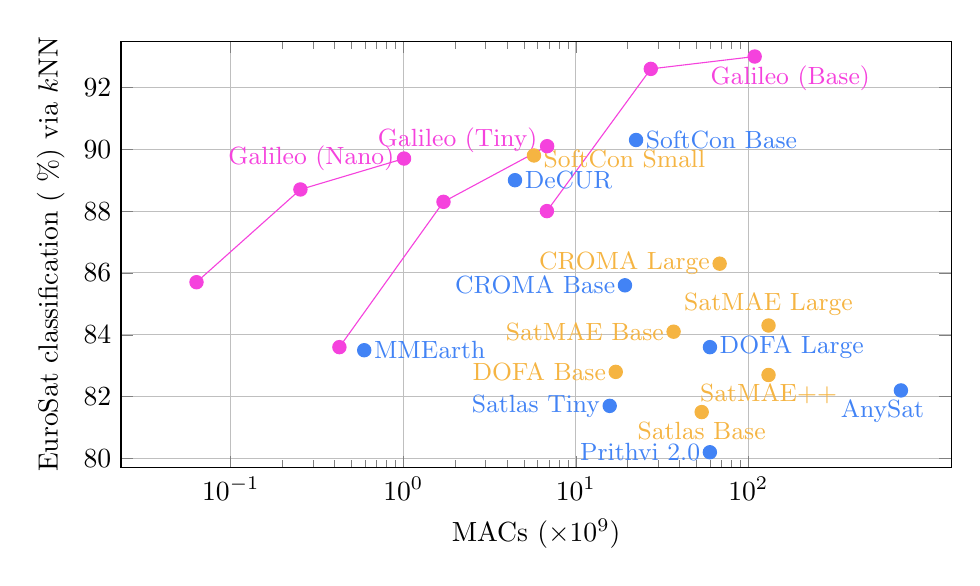
\begin{tikzpicture}
        \begin{axis}[
            xmode=log,
            width=\columnwidth,
            height=7cm,
            xmin=0, xmax=1500, % Limits to cover the full date range
            ymin=79.7, ymax=93.5,
            xtick={0.1, 1, 10, 100},
            % xticklabel style={anchor=north, /pgf/number format/precision=0, /pgf/number format/use comma=false, /pgf/number format/1000 sep={}}, % Ensures no commas and integer formatting
            xlabel={MACs ($
            \times 10^{9}$)},
            ylabel={EuroSat classification (
            \%) via $k$NN},
            grid=major,
        ]
            % Scatter plot points with decimal year representation
            \addplot[only marks, mark=*, mark options={scale=1.2, color=secondcolor}] coordinates {(4.44, 89)}; % DeCur
            \addplot[only marks, mark=*, mark options={scale=1.2, color=thirdcolor}] coordinates {(130.94, 82.7)}; % SatMAEpp
            \addplot[only marks, mark=*, mark options={scale=1.2, color=secondcolor}] coordinates {(15.72, 81.7)}; % Satlas Tiny
            \addplot[only marks, mark=*, mark options={scale=1.2, color=secondcolor}] coordinates {(59.91, 83.6)}; % DOFA Large\
            \addplot[only marks, mark=*, mark options={scale=1.2, color=secondcolor}] coordinates {(19.27, 85.6)}; % CROMA Base
            \addplot[only marks, mark=*, mark options={scale=1.2, color=thirdcolor}] coordinates {(68.18, 86.3)}; % CROMA Large
            \addplot[only marks, mark=*, mark options={scale=1.2, color=secondcolor}] coordinates {(0.59377, 83.5)}; % MMEarth
            \addplot[only marks, mark=*, mark options={scale=1.2, color=thirdcolor}] coordinates {(5.72, 89.8)}; % SoftCon small
            \addplot[only marks, mark=*, mark options={scale=1.2, color=secondcolor}] coordinates {(22.35, 90.3)}; % SoftCon base
            \addplot[only marks, mark=*, mark options={scale=1.2, color=thirdcolor}] coordinates {(36.88, 84.1)}; % SatMAE base
            \addplot[only marks, mark=*, mark options={scale=1.2, color=thirdcolor}] coordinates {(130.94, 84.3)}; % SatMAE large
            \addplot[only marks, mark=*, mark options={scale=1.2, color=thirdcolor}] coordinates {(53.65, 81.5)}; % SatMAE large
            \addplot[only marks, mark=*, mark options={scale=1.2, color=secondcolor}] coordinates {(766.40, 82.2)}; % AnySat
            \addplot[only marks, mark=*, mark options={scale=1.2, color=thirdcolor}] coordinates {(17.04, 82.8)}; % DOFA Base
            \addplot[only marks, mark=*, mark options={scale=1.2, color=secondcolor}] coordinates {(59.84, 80.2)}; % Prithvi Large
            
            \addplot[only marks, mark=*, mark options={scale=1.2, color=ourcolor}] coordinates {(1.01, 89.7)}; % Mercury nano ps 4
            \addplot[only marks, mark=*, mark options={scale=1.2, color=ourcolor}] coordinates {(0.2533, 88.7)}; % Mercury nano ps 8
            \addplot[only marks, mark=*, mark options={scale=1.2, color=ourcolor}] coordinates {(0.0633, 85.7)}; % Mercury nano ps 8
            \addplot[only marks, mark=*, mark options={scale=1.2, color=ourcolor}] coordinates {(6.82, 90.1)}; % Mercury tiny ps 4
            \addplot[only marks, mark=*, mark options={scale=1.2, color=ourcolor}] coordinates {(1.71, 88.3)}; % Mercury tiny ps 8
            \addplot[only marks, mark=*, mark options={scale=1.2, color=ourcolor}] coordinates {(0.42628, 83.6)}; % Mercury tiny ps 16
            \addplot[only marks, mark=*, mark options={scale=1.2, color=ourcolor}] coordinates {(108.82, 93.0)}; % Mercury base ps 4
            \addplot[only marks, mark=*, mark options={scale=1.2, color=ourcolor}] coordinates {(27.20, 92.6)}; % Mercury base ps 8
            \addplot[only marks, mark=*, mark options={scale=1.2, color=ourcolor}] coordinates {(6.80, 88.0)}; % Mercury base ps 16
            \draw[ourcolor,->] (1.01, 89.7) -- (0.2533, 88.7) -- (0.0633, 85.7);
            \draw[ourcolor,->] (6.82, 90.1) -- (1.71, 88.3) -- (0.42628, 83.6);
            \draw[ourcolor,->] (108.82, 93.0) -- (27.20, 92.6) -- (6.80, 88.0);
            % Manually place labels at specified offsets
            \node[anchor=west, text=secondcolor] at (axis cs:4.44, 89) {\small DeCUR};
            \node[anchor=north, text=thirdcolor] at (axis cs:130.94, 82.7) {\small SatMAE++};
            \node[anchor=east, text=secondcolor] at (axis cs:15.72, 81.7) {\small Satlas Tiny};
            \node[anchor=west, text=secondcolor] at (axis cs:59.91, 83.6) {\small DOFA Large};
            \node[anchor=east, text=thirdcolor] at (axis cs:68.18, 86.3) {\small CROMA Large};
            \node[anchor=east, text=secondcolor] at (axis cs:19.27, 85.6) {\small CROMA Base};
            \node[anchor=west, text=secondcolor] at (axis cs:0.59377, 83.5) {\small MMEarth};
            \node[anchor=west, text=thirdcolor] at (axis cs:5.72, 89.7) {\small SoftCon Small};
            \node[anchor=west, text=secondcolor] at (axis cs:22.35, 90.3) {\small SoftCon Base};
            \node[anchor=east, text=thirdcolor] at (axis cs:36.88, 84.1) {\small SatMAE Base};
            \node[anchor=south, text=thirdcolor] at (axis cs:130.94, 84.3) {\small SatMAE Large};
            \node[anchor=north, text=thirdcolor] at (axis cs:53.65, 81.5) {\small Satlas Base};
            \node[anchor=north, text=secondcolor] at (axis cs:600, 82.2) {\small AnySat};
            \node[anchor=east, text=thirdcolor] at (axis cs:17.04, 82.8) {\small DOFA Base};
            \node[anchor=east, text=secondcolor] at (axis cs:59.84, 80.2) {\small Prithvi 2.0};
            
            \node[anchor=east, text=ourcolor] at (axis cs:1.01, 89.7) {\small Galileo (Nano)};
            \node[anchor=east, text=ourcolor] at (axis cs:6.82, 90.3) {\small Galileo (Tiny)};
            \node[anchor=north, text=ourcolor] at (axis cs:175, 93) {\small Galileo (Base)};
        \end{axis}
    \end{tikzpicture}
    \vspace{-10pt}
    \caption{Practitioners can balance model performance with inference-time compute costs by varying the input patch size. This plot shows EuroSat $k$NN results using patch sizes $\{4, 8, 16\}$ compared with inference costs. Compute costs are measured using Multiply-Accumulate operations (MACs) required to encode a single EuroSat instance; note the log scale on the x-axis. Full results are available in Table \ref{tab:eurosat_per_patch}.}
    \label{fig:model_performance}
\end{figure}

\begin{table}[!t]\centering\footnotesize
    \newcommand{\BEST}[1]{\textbf{#1}}
    \newcommand{\SECOND}[1]{\underline{#1}}
    \newcommand{\COLUMNvalues}[2]{
        \def\COLUMNmin{#1}
        \def\COLUMNmax{#2}
        % Reset tracking for this column
        \global\def\COLUMNbest{0}
        \global\def\COLUMNsecond{0}
        \global\def\COLUMNbestrow{0}
        \global\def\COLUMNsecondrow{0}
    }
    \newcommand{\CELLvalue}[3]{
        \ifstrequal{#3}{}
            {
                \csxdef{C#1R#2}{--}
            }{
            % Store the raw value first
            \csxdef{C#1R#2}{#3}
            
            % Update best/second best
            \ifdim #3pt > \COLUMNbest pt
                % Current value is new best
                \xdef\COLUMNsecond{\COLUMNbest}
                \xdef\COLUMNsecondrow{\COLUMNbestrow}
                \xdef\COLUMNbest{#3}
                \xdef\COLUMNbestrow{#2}
            \else
                \ifdim #3pt > \COLUMNsecond pt
                    % Current value is new second best
                    \xdef\COLUMNsecond{#3}
                    \xdef\COLUMNsecondrow{#2}
                \fi
            \fi
            
            % If this is the last row in the column, format all values
            \ifnum#2=5
                \foreach \i in {1,2,3,4,5} {
                    \ifnum\i=\COLUMNbestrow
                        \csxdef{C#1R\i}{\noexpand\BEST{\csuse{C#1R\i}}}
                    \fi
                    \ifnum\i=\COLUMNsecondrow
                        \csxdef{C#1R\i}{\noexpand\SECOND{\csuse{C#1R\i}}}
                    \fi
                }
            \fi
            }
    }
    % Column 1
        \COLUMNvalues{73.4}{75.5}
        \CELLvalue{1}{1}{75.5}
        \CELLvalue{1}{2}{73.4}
        \CELLvalue{1}{3}{73.5}
        \CELLvalue{1}{4}{74.7}
        \CELLvalue{1}{5}{74.8}
        
    % Column 2
        \COLUMNvalues{76.4}{99.3}
        \CELLvalue{2}{1}{98.8}
        \CELLvalue{2}{2}{76.7}
        \CELLvalue{2}{3}{76.4}
        \CELLvalue{2}{4}{97.2}
        \CELLvalue{2}{5}{99.3}

    % Column 3
        \COLUMNvalues{75.5}{85.4}
        \CELLvalue{3}{1}{84.0}
        \CELLvalue{3}{2}{75.5}
        \CELLvalue{3}{3}{84.5}
        \CELLvalue{3}{4}{85.4}
        \CELLvalue{3}{5}{84.2}

    % Column 4
        \COLUMNvalues{16.1}{27.9}
        \CELLvalue{4}{1}{63.0}
        \CELLvalue{4}{2}{66.1}
        \CELLvalue{4}{3}{67.3}
        \CELLvalue{4}{4}{69.0}
        \CELLvalue{4}{5}{73.0}

    \newcommand{\CELLvaluedsaddasdsadasdad}[3]{%
        %\cellcolor{COLMAX!0!COLMED!100!COLMIN}#1
        \FPeval\MIDvalue{(#1+#2)/2}%
        \FPeval\NORMvalue{(#3-#1)*((100)/(#2-#1))}%
        #3
    }
    %
    \caption{Pixel timeseries classification performance via linear probing. The best result is \textbf{bolded} and the second best is \underline{underlined}. The CropHarvest dataset contains a number of modalities in addition to Sentinel-2 optical imagery, including topography, weather and SAR data. We use all modalities each model can support.}
    \label{tab:ts_results}
    \setlength{\tabcolsep}{2pt}
    \resizebox{\linewidth}{!}{\begin{tabular}{
        l
        l
        c%S[table-format=2.2]%1
        c%S[table-format=2.2]%2
        c%S[table-format=2.2]%3
        c%S[table-format=2.2]%4
    }
         & & \multicolumn{3}{c}{CropHarvest} & \\
        \cmidrule(lr){3-5}
        Method & Arch. & \multicolumn{1}{>{\centering\arraybackslash}p{40pt}}{Togo} & \multicolumn{1}{>{\centering\arraybackslash}p{40pt}}{Brazil} & \multicolumn{1}{>{\centering\arraybackslash}p{40pt}}{Kenya} & \multicolumn{1}{>{\centering\arraybackslash}p{40pt}}{Breizhcrops} \\
        \toprule
        Presto & ViT-Presto &  \csuse{C1R1} & \csuse{C2R1} & \csuse{C3R1} & \csuse{C4R1} \\
        AnySat & ViT-Base &  \csuse{C1R2} & \csuse{C2R2} & \csuse{C3R2} & \csuse{C4R2} \\
        \color{ourcolor}\textbf{Galileo} & ViT-Nano & \csuse{C1R3} & \csuse{C2R3} & \csuse{C3R3} & \csuse{C4R3} \\
        \color{ourcolor}\textbf{Galileo} & ViT-Tiny &  \csuse{C1R4} & \csuse{C2R4} & \csuse{C3R4} & \csuse{C4R4} \\
        \color{ourcolor}\textbf{Galileo} & ViT-Base &  \csuse{C1R5} & \csuse{C2R5} & \csuse{C3R5} & \csuse{C4R5} \\
    \end{tabular}}
\end{table}


\subsection{Ablations} \label{sec:ablations}

For all our ablation experiments, we pretrain ViT-Tiny models for $200$ epochs. We select four diverse validation tasks covering segmentation (Sen1Floods11 and MADOS), image classification (EuroSat), and timeseries classification (CropHarvest), using only the validation sets for ablations. 

We begin by ablating our global and local feature learning algorithms in isolation; while the global learning algorithm excels at the classification tasks and the local learning algorithm excels at the segmentation tasks, neither excel at both. We then ablate our combined algorithm, which excels on both the classification and segmentation tasks.

\definecolor{customgray}{gray}{0.5}
\begin{table}[!th]\centering\footnotesize
    \caption{Ablating our \emph{global} feature learning algorithm. MADOS and Sen1Floods11 (\% mIoU) via linear probing. CropHarvest and EuroSat (\% OA) via $k$NN. Our approach in \colorbox{lightour}{pink}. Global feature learning requires contiguous masking and abstract (deep) targets.}
    \label{tab:global_ablation}
    \setlength{\tabcolsep}{2pt}
    \resizebox{\columnwidth}{!}{
        \begin{tabular}{
            c%S[table-format=2.2]
            c%S[table-format=2.2]
            c%S[table-format=2.2]
            r%S[table-format=2.2]%1
            r%S[table-format=2.2]%2
            r%S[table-format=2.2]%3
            r%S[table-format=2.2]%4
        }
            \makecell{masking\\strategy} &
            \makecell{target enc.\\exit depth} &
            \makecell{loss\\function} &
            \textcolor{customgray}{MADOS} & 
            \textcolor{customgray}{Floods} & 
            CropH. & 
            EuroSat \\
            \toprule
            \cellcolor{lightour} space+time & \cellcolor{lightour}varied & \cellcolor{lightour}AllDisc & \textcolor{customgray}{58.91} & \textcolor{customgray}{76.92} & 88.72 & 89.50 \\
            random & \cellcolor{lightour}varied & \cellcolor{lightour}AllDisc & \textcolor{customgray}{11.71} & \textcolor{customgray}{69.62} & 82.12 & 17.40 \\
            \scriptsize{random+space+time} & \cellcolor{lightour}varied & \cellcolor{lightour}AllDisc & \textcolor{customgray}{22.87} & \textcolor{customgray}{71.62} & 76.53 & 66.30 \\
            \cellcolor{lightour} space+time & $0$ & \cellcolor{lightour}AllDisc & \textcolor{customgray}{61.73} & \textcolor{customgray}{76.66} & 85.79 & 86.90 \\
            \cellcolor{lightour}space+time & $6$ & \cellcolor{lightour}AllDisc & \textcolor{customgray}{63.83} & \textcolor{customgray}{76.93} & 88.17 & 89.20 \\
            \cellcolor{lightour}space+time & $12$ & \cellcolor{lightour}AllDisc & \textcolor{customgray}{60.35} & \textcolor{customgray}{77.19} & 87.30 & 87.90 \\
            \cellcolor{lightour}space+time & \cellcolor{lightour}varied & MSE & \textcolor{customgray}{62.35} & \textcolor{customgray}{76.78} & 86.02 & 87.20 \\
            \cellcolor{lightour}space+time & \cellcolor{lightour}varied & PatchDisc & \textcolor{customgray}{25.74} & \textcolor{customgray}{71.68} & 75.30 & 62.50 \\
        \end{tabular}
        }
        \vspace{1pt}
\end{table}


\textbf{Ablations within our global feature learning algorithm.} We find that replacing our approach by random masking or PatchDisc significantly harms classification. Similarly our AllDisc loss outperforms MSE (used in I-JEPA) by $2.3\%$ on EuroSat and $2.7\%$ on CropHarvest (Tab.~\ref{tab:global_ablation}). Using only linear projections for target processing reduces performance by $2.6\%$ on EuroSat and $2.93\%$ on CropHarvest, confirming the importance of targeting higher-level features for classification.

\definecolor{customgray}{gray}{0.5}
\begin{table}[!th]\centering\footnotesize
    \caption{Ablating our \emph{local} feature learning algorithm. MADOS and Sen1Floods11 (\% mIoU) via linear probing. CropHarvest and EuroSat (\% OA) via $k$NN. Our approach in \colorbox{lightour}{pink}. Local feature learning requires random masking and pixel (shallow) targets.}
    \label{tab:local_ablation}
    \setlength{\tabcolsep}{2pt}
    \resizebox{\columnwidth}{!}{
        \begin{tabular}{
            c
            c
            c
            r
            r
            r
            r
        }
            \makecell{masking\\strategy} &
            \makecell{target enc.\\exit depth} &
            \makecell{loss\\function} &
            MADOS & 
            Floods & 
            \textcolor{customgray}{CropH.} & 
            \textcolor{customgray}{EuroSat} \\
            \toprule
            \cellcolor{lightour} random & \cellcolor{lightour}$0$ & \cellcolor{lightour}PatchDisc & 71.48 & 77.39 & \textcolor{customgray}{86.77} & \textcolor{customgray}{86.90} \\
            \scriptsize{random+space+time} & \cellcolor{lightour}$0$ & \cellcolor{lightour}\cellcolor{lightour}PatchDisc & 68.63 & 77.82 & \textcolor{customgray}{85.31} & \textcolor{customgray}{88.80} \\
            space+time & \cellcolor{lightour}$0$ & \cellcolor{lightour}PatchDisc & 62.25 & 77.22 & \textcolor{customgray}{86.82} & \textcolor{customgray}{87.00} \\
            \cellcolor{lightour}random & $6$ & \cellcolor{lightour}PatchDisc & 58.53 & 75.66 & \textcolor{customgray}{76.58} & \textcolor{customgray}{65.40} \\
            \cellcolor{lightour}random & $12$ & \cellcolor{lightour}PatchDisc & 11.65 & 72.60 & \textcolor{customgray}{71.92} & \textcolor{customgray}{27.50} \\
            \cellcolor{lightour}random & varied & \cellcolor{lightour}PatchDisc & 8.25 & 68.89 & \textcolor{customgray}{77.83} & \textcolor{customgray}{18.40} \\
            \cellcolor{lightour}random & \cellcolor{lightour}$0$ & MSE & 65.34 & 77.09 & \textcolor{customgray}{86.71} & \textcolor{customgray}{87.40} \\
            \cellcolor{lightour}random & \cellcolor{lightour}$0$ & AllDisc & 70.12 & 77.26 & \textcolor{customgray}{85.27} & \textcolor{customgray}{88.20} \\
        \end{tabular}
        }
    \vspace{-15pt}
\end{table}

\paragraph{Ablations within our local feature learning algorithm.} Space and time masking significantly degrade MADOS performance. Cross-batch negative sampling (AllDisc) slightly harms segmentation (Tab. \ref{tab:local_ablation}). Using more encoder layers for target processing (as in LatentMIM's full $12$-layer approach) fails to learn useful representations, validating our targeting of low-level features through linear projections alone.

\definecolor{customgray}{gray}{0.5}
\begin{table}[!th]\centering\footnotesize
    \caption{Ablating our \emph{combined} feature learning algorithm. MADOS and Sen1Floods11 (\% mIoU) via linear probing. CropHarvest and EuroSat (\% OA) via $k$NN. Winner in \colorbox{lightour}{pink}; naive combination in \colorbox{gray!20}{gray}.}
    \vspace{15pt}
    \label{tab:combined_ablation}
    \setlength{\tabcolsep}{2pt}
    \resizebox{\columnwidth}{!}{
        \begin{tabular}{
            c%S[table-format=2.2]%2
            c%S[table-format=2.2]%3
            c%S[table-format=2.2]%4
            c%S[table-format=2.2]%5
            r%S[table-format=2.2]%1
            r%S[table-format=2.2]%2
            r%S[table-format=2.2]%3
            r%S[table-format=2.2]%4
        }   
            \makecell{global\\loss} &
            \makecell{local\\loss} &
            \makecell{share\\predictors} &
            \makecell{target\\context} &
            MADOS & 
            Floods & 
            CropH. & 
            EuroSat \\
            \toprule
            \rowcolor{gray!20} AllDisc & PatchDisc & no & dec. & 63.54 & 76.95 & 86.98 & 89.30 \\
            \rowcolor{lightour} PatchDisc & PatchDisc & no & all & 67.79 & 77.66 & 87.87 & 91.00 \\
            PatchDisc & PatchDisc & no & dec. & 36.98 & 74.21 & 85.49 & 83.30 \\
            PatchDisc & PatchDisc & no & \scriptsize{dec.+enc.} & 63.41 & 77.36 & 85.87 & 89.30 \\
            PatchDisc & PatchDisc & yes & all & 67.04 & 78.23 & 85.23 & 88.50 \\
            AllDisc & AllDisc & no & all & 67.88 & 77.08 & 86.61 & 89.50 \\
            MSE & MSE & no & all & 62.36 & 77.17 & 86.28 & 88.70 \\
        \end{tabular}
        }

\end{table}

\textbf{Ablations to our combined algorithm.} Leveraging PatchDisc for both objectives and providing the target encoder with all available tokens outperforms naively combining our prior global and local objectives (Tab.~\ref{tab:combined_ablation}). Not sharing predictor parameters across objectives is optimal. Interestingly, our dual-objective strategy achieves successful training runs more consistently. We believe this is a valuable finding beyond our RS focus, as improving latent prediction SSL is an active research area \cite{wei2024towards, littwin2024enhancingjepasspatialconditioning, mo2024connecting}.

\section{Related Work and Background}

\textbf{Self-Supervised Learning.} Reconstructing a masked or noised input is a common form of self-supervised pretraining, both for natural language \cite{devlin2018bert, radfordimproving, skipgram} and natural imagery \cite{xie2022simmim, he2022masked, vincent2008extracting}. The most successful such framework for natural imagery is masked autoencoding (MAE, \citet{he2022masked}), which encodes a subset of patches, then predicts the hidden patches with a decoder conditioned on the hidden patch locations. 
%
Contrastive learning \cite{le2020contrastive, oord2018representation, chen2020simple, chopra2005learning} is a different approach to learning representations, which encodes samples augmented in two different ways, then attracts the representations of the same sample (called positives), and repels the representations of different samples (called negatives). 
%
Models pretrained with MAE typically outperform contrastive learning under finetuning evaluations, whereas the reverse is generally true under frozen feature evaluations \cite{park2023what, he2022masked, garrido2024learning}. 

A third paradigm has recently emerged that makes predictions in a latent space, like contrastive learning, and conditions the prediction on the sample's transformation, like MAE. For instance, I-JEPA \cite{assran2023self} achieves strong performance under both finetuning and frozen feature evaluations; essentially, I-JEPA modifies MAE to predict patch \emph{representations}, computed by the encoder's exponential moving average. LatentMIM \cite{wei2024towards} showed that I-JEPA pretraining is unstable and can be improved by their patch discrimination objective; PatchDisc attracts patch representations of the same location within an image, and repels patch representations of the same sample but different locations. Our approach falls into this third category, offering a novel learning algorithm tailored for RS.

\textbf{Pretrained RS Models.} \label{sec:pretrained_rs} SatMAE \cite{cong2022satmae} adapted MAE to multispectral satellite imagery. SatMAE++ \cite{noman2024rethinking} improved over SatMAE by reconstructing upsampled inputs. Prithvi 2.0 \cite{szwarcman2024prithvi} applied MAE to Harmonized Landsat and Sentinel (HLS) multispectral imagery. CROMA \cite{fuller2024croma} adapted contrastive captioners \cite{yu2022coca} to jointly model multispectral and SAR data. SoftCon \cite{wang2024multi} adapted supervised contrastive learning \cite{khosla2020supervised, zhang2022use} to separately model multispectral and SAR data. MMEarth \cite{nedungadi2024mmearth} adapted convolutional MAEs \cite{woo2023convnext} to reconstruct images and other RS data. Presto \cite{tseng2023lightweight} adapted MAE to pixel-timeseries of multispectral, SAR, and other RS data. Satlas \cite{bastani2023satlaspretrain} adapted Swin transformers \cite{liu2021swin} to multispectral (and optionally multiple) images using multi-task supervised pretraining. DOFA \cite{xiong2024neural} adapted MAE to separately model multispectral, SAR, and high-resolution RGB images. DeCUR \cite{wang2024decoupling} adapted Barlow Twins \cite{zbontar2021barlow} to separately model multispectral and SAR imagery. 

While there are other pretrained models, they ingest only RGB images \cite{reed2023scale, tang2024cross, mendieta2023towards}, have not published pretrained weights \cite{guo2024skysense, han2024bridging}, or have been surpassed by above-cited newer models \cite{fuller2022satvit, wang2023ssl4eo, ayush2021geography, manas2021seasonal, jean2019tile2vec, astruc2024omnisat, jakubik2023foundation}. 

AnySat \cite{astruc2024anysat} is concurrent with our work and shares the same spirit.
It combines I-JEPA \cite{assran2023self} and contrastive learning objectives to pretrain an RS model.
AnySat is pretrained on data from more satellites, but does not include other modalities modeled by Galileo.

\section{Conclusion}

In this work, we identify two requirements for the application of pretrained models in a wide range of RS contexts: (i) the ability to flexibly process different modalities and input shapes, and (ii) the ability to model RS phenomena which occur at very different scales. To meet these requirements, we present the Galileo family of pretrained RS models. 

We achieve these requirements by innovating on (i) the pretraining dataset used to train the Galileo models, (ii) the model architecture, allowing the model to flexibly ingest a highly multimodal dataset that varies in both space and time, and (iii) the SSL algorithm, to encourage the model to learn phenomena occurring at vastly different scales. 

We run hundreds of evaluations --- including extensive sweeps of baseline pretrained RS models --- to robustly demonstrate Galileo's performance across a wide range of domains, modalities, and task types. We run thorough ablations of our method. We hope the resulting insights will serve the SSL community beyond RS.

The model weights, pretraining code, pretraining data and evaluation code are open sourced at \href{https://github.com/nasaharvest/galileo}{github.com/nasaharvest/galileo}.

\section*{Impact Statement}

Applications of machine learning to RS span a range of societally important applications, from species distribution modelling \cite{teng2024satbird} to disaster management \citep{kansakar2016review}. By providing a set of RS models which can perform well even when few labels are available, we hope to enable RS practitioners to continue exploring and deploying these applications. We take several steps to encourage the adoption of these models, including training the models on publicly available RS data and training a diversity of model sizes so that they can be used in compute-constrained environments.

\citet{tuia2023artificial} highlight that a risk of these models is that they can be used to collect information about populations so that decisions are made without their involvement. We encourage the deployment of Galileo in collaboration with local communities and stakeholders \citep{maui,kshirsagar2021becoming,nakalembe2023considerations}.

\bibliography{example_paper}
\bibliographystyle{icml2024}


%%%%%%%%%%%%%%%%%%%%%%%%%%%%%%%%%%%%%%%%%%%%%%%%%%%%%%%%%%%%%%%%%%%%%%%%%%%%%%%
%%%%%%%%%%%%%%%%%%%%%%%%%%%%%%%%%%%%%%%%%%%%%%%%%%%%%%%%%%%%%%%%%%%%%%%%%%%%%%%
% APPENDIX
%%%%%%%%%%%%%%%%%%%%%%%%%%%%%%%%%%%%%%%%%%%%%%%%%%%%%%%%%%%%%%%%%%%%%%%%%%%%%%%
%%%%%%%%%%%%%%%%%%%%%%%%%%%%%%%%%%%%%%%%%%%%%%%%%%%%%%%%%%%%%%%%%%%%%%%%%%%%%%%
\newpage
\appendix
\onecolumn

\section{Methodology details}

\subsection{The Galileo SSL algorithm}

We adopt a latent prediction framework inspired by \citet{assran2023self}, \citet{garrido2024learning}, and \citet{wei2024towards}, which operates as follows: \circlednum{1} Given a batch of samples, we construct two \emph{different} views of each sample, $\mathbf{x}_1 \in \mathbb{R}^{L_1 \times D}$ and $\mathbf{x}_2 \in \mathbb{R}^{L_2 \times D}$. \circlednum{2} Our ``online'' encoder computes patch encodings $\mathbf{z}_1 = \mathbf{E}(\mathbf{x}_1)$, while our ``target'' encoder --- an exponential moving average of the online encoder --- computes target patch encodings $\mathbf{z}_2 = \mathbf{E}_{\text{EMA}}(\mathbf{x}_2)$. \circlednum{3} A predictor transformer $\mathbf{P}$ receives the target view's position, time, month, and channel group embeddings $\mathtt{e}_2 \in \mathbb{R}^{L_2 \times D}$ as placeholder queries and predicts patch encodings $\mathbf{p} \in \mathbb{R}^{L_2 \times D}$ by cross-attending to the online patch encodings, i.e., $\mathbf{p}=\mathbf{P}(\mathtt{e}_2, \mathbf{z}_1)$. \circlednum{4} The predictions $\mathbf{p}$ and targets $\mathbf{z}_2$ are compared to compute a loss $\mathcal{L}(\mathbf{p}, \mathbf{z}_2)$ that updates the online encoder. 

We adapt this latent prediction framework for learning local and global features. We outline those adaptations below.

\subsubsection{Learning Global Features} \label{app:global}

We design this algorithm to learn abstract, lower-frequency features suited for classification applications. \circlednum{1} View construction involves: \circlednum{a} uniformly sampling the number of channel groups $N \in \{2,3,\ldots,17\}$, \circlednum{b} randomly selecting $N$ channel groups (e.g., RGB, SAR, ERA5), \circlednum{c} repeating steps (a-b) for the target encoder while excluding overlapping channel groups, \circlednum{d} applying either spatial or temporal masking, and \circlednum{e} tokenizing both views to obtain $\mathbf{x}_1$ and $\mathbf{x}_2$. Space masking samples masks across space while maintaining consistency across channel groups and time; time masking does the same across time while maintaining consistency across channel groups and space. \circlednum{2}-\circlednum{3} Following our general framework, we compute $\mathbf{z}_{1}$ and $\mathbf{p}$, and compute targets using varied exit depths from the target encoder, $\mathbf{E}_{\text{EMA}}^{\ell}$. \circlednum{4} We use our AllDisc loss (defined in Section \ref{subsection:global} as:

\makebox[\columnwidth]{
$\mathcal{L}_{global} = \text{AllDisc}(\mathbf{P}(\mathtt{e}_2, \mathbf{E}(\mathbf{x}_1)),\text{sg}(\mathbf{E}_{\text{EMA}}^{\ell}(\mathbf{x}_2)))$
}

\subsubsection{Learning Local Features} \label{app:local}
We design this algorithm to learn fine-grained, higher-frequency features suited for segmentation applications. \circlednum{1} View construction involves: \circlednum{a} tokenizing the entire sample, and \circlednum{b} randomly selecting $5\%$ of tokens for $\mathbf{x}_1$ and $50\%$ for $\mathbf{x}_2$. \circlednum{2}-\circlednum{3} Following our general framework, we compute $\mathbf{z}_{1}$ and $\mathbf{p}$, but compute targets using only the target encoder's linear projection, i.e., $\mathbf{E}_{\text{EMA}}^{proj}$ --- skipping transformer blocks such that the predictor targets low-level features. \circlednum{4} We use LatentMIM's PatchDisc loss, tasking the model to discriminate between patches on the basis of low-level features alone:

\makebox[\columnwidth]{
$\mathcal{L}_{local} = \text{PatchDisc}(\mathbf{P}(\mathtt{e}_2, \mathbf{E}(\mathbf{x}_1)), \text{sg}(\mathbf{E}_{\text{EMA}}^{proj}(\mathbf{x}_2)))$
}

\subsubsection{Combining Local and Global Objectives}

As noted in Section \ref{sec:combined}, our combined method alternates between the local and global objectives during pretraining:

\makebox[\columnwidth]{
$\mathcal{L}_{Galileo} = \frac{1}{2}(\mathcal{L}_{global} + \mathcal{L}_{local})$
}


\section{Pretraining details}

\subsection{A globally sampled pretraining dataset}\label{app:pretraining_dataset}

To construct the Galileo dataset, we split the global WorldCover map \cite{zanaga2022esa} into $1000 \times 1000$ pixels ($10km \times 10km$) tiles. For each tile, we compute two feature sets: \circlednum{1} the number of pixels within each WorldCereal classification class, and \circlednum{2} the latitude and longitude of the tile. We use these features to train a $k$=\num{150000} $k$-means clustering algorithm, and select the tiles closest to the centroid of each cluster. This yields \num{150000} training points, of which 85\% (\num{127155}) are successfully exported using Google Earth Engine \cite{gorelick2017google}. By including both the pixel counts and the latitude and longitudes as features to the $k$-means algorithm, we ensure both the semantic and geographic diversity of the model's training points --- Figure \ref{fig:data} shows a chloropleth map of the exported points.

We use this sampling procedure to construct a rich dataset to pretrain our model. This dataset consists of \num{9} RS inputs, ranging from directly sensed inputs (such as Sentinel-2 optical imagery) to semantically dense maps (such as the Dynamic World landcover maps) --- these are discussed in detail in Section \ref{sec:dataset}. Table \ref{tab:data_ablation} studies the impact of each of these modalities on the model's downstream performance, by pretraining the global-local model (Section \ref{sec:combined}) while omitting a single data product.

\definecolor{customgray}{gray}{0.5}
\begin{table}[!th]\centering\footnotesize
    \caption{Ablating the Galileo dataset. MADOS and Sen1Floods11 (\% mIoU) via linear probing. CropHarvest and EuroSat (\% OA) via $k$NN.}\label{tab:data_ablation}
    \setlength{\tabcolsep}{2pt}
    \begin{tabular}{
        l%S[table-format=2.2]
        r%S[table-format=2.2]%1
        r%S[table-format=2.2]%2
        r%S[table-format=2.2]%3
        r%S[table-format=2.2]%4
    }
    \toprule
        \parbox{1.7cm}{\raggedright{Removed\\input}} &
        \parbox{1.7cm}{\raggedleft{MADOS}} & \parbox{1.7cm}{\raggedleft{Sen1Floods11}} & \parbox{1.7cm}{\raggedleft{CropHarvest}} & \parbox{1.7cm}{\raggedleft{EuroSat}} \\
        \midrule
        \rowcolor{lightour} None & 67.79 & 77.66 & 87.87 & 91.00 \\
        S1 & 67.67 & \textcolor{customgray}{N/A} & 85.27 & 90.20 \\
        NDVI & 67.89 & 78.10 & 88.32 & 90.00 \\
        ERA5 & 68.10 & 77.10 & 87.14 & 91.20 \\
        TerraClim & 61.30 & 74.90 & 82.78 & 81.20 \\
        VIIRS & 63.48 & 74.52 & 84.10 & 81.10 \\
        SRTM & 66.14 & 77.62 & 86.74 & 91.00 \\
        DynamicWorld & 67.24 & 77.86 & 87.80 & 89.30 \\
        WorldCereal & 65.94 & 77.56 & 87.71 & 89.60 \\
        LandScan & 60.74 & 77.45 & 87.89 & 91.10 \\
    \end{tabular}
\end{table}


\subsection{Implementation}

\begin{wrapfigure}{l}{0.4\linewidth}
    \includegraphics[width=\linewidth]{pics/exported_training_points_all.png}
    \caption{The number of exported training points per H3 cell \cite{h3} at resolution $=2$ . We sample from the entire globe, aiming for semantic diversity (defined by the WorldCover landcover map classes \cite{zanaga2022esa}) and geographic coverage.}
    \label{fig:data}
\end{wrapfigure}

All models are trained on single H100 GPUs (model sizes and training times are described in Table \ref{tab:size_cost}). We use an effective batch size of $512$, which consists of a minibatches of $128$ instances augmented and repeated $4$ times \cite{hoffer2019augment}. For data augmentations, we randomly apply vertical and horizontal flipping and 90-degree rotations to each instance. When repeating the data, we first randomly select a patch size $P \in [1, 2, 3, 4, 5, 6, 7, 8]$. We then randomly select a (size, timestep) combination $(S, T) \in [(4, 12), (5, 6), (6, 4), (7, 3), (9, 3), (12, 3)]$. We then randomly subset spatially height $H = P \times S$, width $W = P \times S$ and timesteps $T$ from each instance in the batch.

\begin{table}[!t]\centering
    \scriptsize
    %
    \caption{Configurations of our ViT models and associated pretraining costs. GPU-hours describes the number of GPU-hours required to pretrain each model for $500$ epochs on an H100 GPU.}
    \label{tab:size_cost}
    % \setlength{\tabcolsep}{2pt}
    % \resizebox{\linewidth}{!}{\begin{tabular}{lccccc}
    {\begin{tabular}{lccccc}
       architecture & blocks & dim & heads & params & GPU-hours \\
         \toprule
         ViT-Nano & 4 & 128 & 8 & 0.8M & 200 \\
         % ViT-Tiny \cite{touvron2022deit} & 12 & 192 & 3 & 5.3M & 259 \\
         % ViT-Base \cite{dosovitskiy2021an} & 12 & 768 & 12 & 85M & 573 \\
         ViT-Tiny & 12 & 192 & 3 & 5.3M & 259 \\
         ViT-Base & 12 & 768 & 12 & 85.0M & 573 \\
    \end{tabular}}
\end{table}


We use bfloat16 precision, and the AdamW optimizer with $\beta_1 = 0.9$ and $\beta_2 = 0.999$ with gradient clipping. We warmup our learning rate for 30 epochs to a maximum learning rate before applying a cooldown via a cosine decay schedule. We use exponential moving averaging (EMA) to update our target encoder with a momentum value of 0.996 which linearly increases to 1 throughout pretraining following \citet{assran2022masked}.

For all ablations (Section \ref{sec:ablations}), we pretrain a ViT-Tiny model for $200$ epochs to a maximum learning rate of $2 \times 10^{-3}$ and use a weight decay of $0.02$. For the final Galileo models, we pretrain the models for $500$ epochs and conduct a sweep of $[\textrm{learning rate} \times \textrm{weight decay}]$. For the ViT-Nano and ViT-Tiny architectures, we sweep $\textrm{learning rates} \in [1\times 10^{-3}, 2\times 10^{-3}, 3\times 10^{-3}]$ and $\textrm{weight decays} \in [1\times 10^{-2}, 2\times 10^{-2}, 3\times 10^{-2}]$. For the ViT-Base architecture, we sweep $\textrm{learning rates} \in [1\times 10^{-4}, 3\times 10^{-4}, 1\times 10^{-3}, 2\times 10^{-3}, 3\times 10^{-3}]$ and $\textrm{weight decays} \in [1\times 10^{-2}, 2\times 10^{-2}, 3\times 10^{-2}]$.

\section{Evaluation details} 
\label{app:eval_details}

\subsection{Implementation}
To ensure consistent experimental settings when comparing pretrained models, we rerun all evaluations under identical conditions. For the $k$NN probing, we follow the implementation of \citet{gwilliam2022beyond} --- we use the pretrained models to compute representations of the test data (as values) and training data (as keys) --- we then use the keys to classify the test data. Following \citet{fuller2024croma} and \citet{reed2023scale}, we use $k=20$. When linear probing, we use the pretrained models to compute representations of the training data and use this to train linear probes. We sweep learning rates when training the linear probes ($\{1, 3, 4, 5\} \times 10^{\{-4, -3, -2, -1\}}$) and apply the trained linear probes to the computed representations of the test data. When finetuning, we sweep learning rates when finetuning ($\{1, 3, 6\} \times 10^{\{-5, -4, -3\}}$) and apply the finetuned models to the test data.

\subsection{Evaluation Datasets}

We evaluate our models on the datasets described below. For all GeoBench-modified datasets \cite{lacoste2024geo} - m-Eurosat, m-BigEarthnet, m-So2Sat, m-Brick-Kiln, m-Cashew-Plant and m-SA-Crop-Type, we use the training, validation and test splits shared by GeoBench. In addition, we use the $1\%$, $5\%$ and $20\%$ partitions shared by GeoBench.

\begin{itemize}
\item \textbf{m-EuroSat} \cite{helber2019eurosat}: The full training set consists of \num{2000} images, with \num{1000} images in the validation and test sets. Images are $64 \times 64$ pixels.
\item \textbf{m-BigEarthNet} \cite{sumbul2019bigearthnet}: The full training set consists of \num{20000} images, with \num{1000} images in the test set. Images are $120 \times 120$ pixels.
\item \textbf{m-So2Sat} \cite{zhu2020so2sat}: The full training set consists of \num{19992} images (with \num{986} images in the test set), and images are $32 \times 32$ pixels.
\item \textbf{m-Brick-Kiln} \cite{lee2021scalable}: The full training set consists of \num{15063} images, with \num{999} images in the test set. Images are $64 \times 64$ pixels.
\item \textbf{m-Cashew-Plant} \cite{yin2023mapping}: The full training set consists of \num{1350} images, with \num{50} images in the test set. Images are $256 \times 256$; we subtile them into $64 \times 64$ images.
\item \textbf{m-SA-crop-type} (\href{https://source.coop/repositories/esa/fusion-competition}{link}): The full training set consists of \num{3000} images, with \num{93} images in the test set. Images are $256 \times 256$; we subtile them into $64 \times 64$ images.
\item \textbf{MADOS} \cite{kikaki2024detecting}: The full MADOS dataset consists of \num{2804} $140 \times 140$ images, extracted from \num{174} Sentinel-2 scenes. We use the train/val/test splits from MADOS ($50\%$/$25\%$/$25\%$) --- each split was created as a representative subset of the entire MADOS dataset. In addition, we subtile each image into $80 \times 80$ images.
\item \textbf{PASTIS} \cite{garnot2021panoptic}: The full PASTIS dataset consists of \num{2433} $128 \times 128$ timeseries, with 38-61 timesteps per timeseries. We subtile each timeseries spatially into $64 \times 64$ images. In addition, we compute monthly aggregations of the timeseries. \citet{garnot2021panoptic} share 5 folds of the data; we use folds $\{1, 2, 3\}$ for training, \num{4} for validation and \num{5} for testing. When applying single-timestep models to this dataset, we additionally sweep pooling methods to pool per-timestep encodings (as described in Section \ref{app:eval_details}).
\item \textbf{Breizhcrops} \cite{russwurm2019breizhcrops}: The Breizhcrops dataset consists of pixel-timeseries in \num{4} NUTS-3 regions in Brittany, France. We use \num{2} for training (FRH01, with \num{178613} parcels and FRH02 with \num{140645} parcels). We use FRH03 (\num{166391} parcels) for validation and FRH04 (\num{122614} parcels) for testing. The dataset consists of variable sequence lengths; we compute monthly aggregations of the timeseries.
\item \textbf{CropHarvest} \cite{tseng2021cropharvest}: The CropHarvest dataset consists of \num{3} pixel-timeseries tasks: (i) crop vs. non crop in Togo, with \num{1319} samples in the training set and \num{306} samples in the test set, (ii) maize vs. rest in Kenya with \num{1345} samples in the training set and \num{1942} m$^2$ of densely labelled pixels in the test set, and (iii) coffee vs. rest in Brazil with \num{794} samples in the training set and \num{4.2} km$^{2}$ of densely lablled pixels in the test set.
\end{itemize}

\subsection{Comparing to baseline models}

\citet{Corley_2024_CVPR} found that input-image sizes and feature scaling methods can have significant impacts on the performance of pretrained RS models. We therefore resize all input images to the sizes that the models were pretrained on. In addition, we treat feature scaling methods as an additional hyperparameter, and sweep it in addition to the learning rates (where those are applicable, i.e. for linear probing and finetuning). Finally, the PASTIS dataset consists of multiple timesteps of optical imagery. Since all benchmark models (except AnySat) cannot ingest the full timeseries natively, we use multiple forward passes. We select two methods for combining the outputs of these forward passes - \circlednum{1} a mean of the encodings, and \circlednum{2} a max, following \citet{bastani2023satlaspretrain}.

The reported test results are therefore computed by sweeping the cross product of the following hyperparameters:
$$
[\textrm{Learning Rate}] \times [\textrm{Temporal aggregations}]
$$

We select all hyperparameters using the validation sets in the downstream datasets.

In addition to conducting this sweep, we run the linear probes 5 times and average the results. When running the linear probe, we sweep the learning rate and feature scaling method concurrently for the first run. We select the feature scaling method from this first run, and fix it for all subsequent runs. We then select the best other hyperparameters per run, and aggregate these to obtain our final results.

We run this sweep for all evaluation datasets with the exception of the CropHarvest tasks; these consist of small training sets and no validation sets against which the hyperparameters can be selected. We therefore follow \citet{tseng2023lightweight} in using the same feature scaling methods as was used during pretraining, and using scikit-learn's regression algorithm with default parameters \cite{pedregosa2011scikit} for all models.

\subsubsection{Feature Scaling}
The pretrained models we benchmark against apply either standardization (MMEarth, DOFA, AnySat and Presto) or normalization (all other models) during pretraining. We sweep the following normalization statistics, either via standardization on normalization depending on the pre-training procedure: \circlednum{1} statistics from the downstream datasets, \circlednum{2} SatMAE pretraining statistics, \circlednum{3} SSL4EO \cite{wang2023ssl4eo} statistics, \circlednum{4} Galileo pretraining dataset statistics, \circlednum{5} Presto pretraining dataset statistics. For all of these statistics, we additionally sweep standard deviation multipliers. Prithvi 2.0 statistics only cover a subset of Sentinel-2 bands; we therefore only include those statistics in the sweeps for the Prithvi 2.0 model.

\section{Results} 

\begin{wraptable}{r}{0.5\linewidth}
    % if we have this table in a seperate .tex file, wraptable doens't work.
    \caption{Galileo m-Eurosat classification test performance (\%) as a function of patch size measured via $k$NN for different training set \%s. MACs required to process a single EuroSat instance are also recorded; by selecting the model size and patch size, practitioners can make trade offs between model performance and inference costs.}
    \label{tab:eurosat_per_patch}
    \resizebox{\linewidth}{!}{{\begin{tabular}{lcccccc}
        \toprule
       Arch. & patch size & GMACs & 100 \% & 20 \% & 5\% & 1\% \\
         \toprule
         \multirow{2}*{ViT-Nano} & 8 & 0.25 & 88.7 & 81.9 & 55.0 & 38.5 \\
         & 16 & 0.06 & 85.7 & 79.3 & 56.0 & 41.1 \\
         \midrule
         \multirow{2}*{ViT-Tiny} & 8 & 1.71 & 88.3 & 83.0 & 59.7 & 41.3 \\
         & 16 & 0.43 & 83.6 & 78.4 & 50.1 & 33.8 \\
         \midrule
         \multirow{2}*{ViT-Base} & 8 & 27.20 & 92.6 & 88.3 & 72.4 & 56.9 \\
         & 16 & 6.80 & 88.0 & 82.4 & 58.6 & 48.9 \\
         \bottomrule
    \end{tabular}}}
\end{wraptable}


We include full results for the image classification tasks (Table \ref{tab:knn_full}) and segmentation tasks (Table \ref{tab:seg_results_full}). In addition, full results for the m-Eurosat dataset with varying patch sizes are recorded in Table \ref{tab:eurosat_per_patch} - these values are used in Figure \ref{fig:model_performance}.

We rank the models in Table \ref{tab:ranks}. When ranking the models, we compute the average rank of each model across each dataset and partition.

\begin{table*}\centering\footnotesize
    \newcommand{\BEST}[1]{\textbf{#1}}
    \newcommand{\SECOND}[1]{\underline{#1}}
    \newcommand{\COLUMNvalues}[2]{
        \def\COLUMNmin{#1}
        \def\COLUMNmax{#2}
        % Reset tracking for this column
        \global\def\COLUMNbest{0}
        \global\def\COLUMNsecond{0}
        \global\def\COLUMNbestrows{}
        \global\def\COLUMNsecondrows{}  % Changed to store multiple second-best rows
    }
    \newcommand{\CELLvalue}[3]{
        \ifstrequal{#3}{}
            {
                \csxdef{C#1R#2}{--}
            }{
            % Store the raw value first
            \csxdef{C#1R#2}{#3}
    
            % Update best/second best
            \ifdim #3pt > \COLUMNbest pt
                % Current value is new best
                \xdef\COLUMNsecond{\COLUMNbest}
                \xdef\COLUMNsecondrows{\COLUMNbestrows}  % Old best becomes second
                \xdef\COLUMNbest{#3}
                \xdef\COLUMNbestrows{#2}
            \else
                \ifdim #3pt = \COLUMNbest pt
                    % Tie for best
                    \xdef\COLUMNbestrows{\COLUMNbestrows,#2}
                \else
                    \ifdim #3pt = \COLUMNsecond pt
                        % Tie for second best
                        \xdef\COLUMNsecondrows{\COLUMNsecondrows,#2}
                    \else
                        \ifdim #3pt > \COLUMNsecond pt
                            % New second best
                            \xdef\COLUMNsecond{#3}
                            \xdef\COLUMNsecondrows{#2}
                        \fi
                    \fi
                \fi
            \fi
    
            % If this is the last row in the column, format all values
            \ifnum#2=18
                % Handle best values
                \foreach \bestrow in \COLUMNbestrows {
                    \csxdef{C#1R\bestrow}{\noexpand\BEST{\csuse{C#1R\bestrow}}}
                }
                % Handle second best values
                \foreach \secondrow in \COLUMNsecondrows {
                    \csxdef{C#1R\secondrow}{\noexpand\SECOND{\csuse{C#1R\secondrow}}}
                }
            \fi
            }
    }
    % Column 1
        \COLUMNvalues{0}{100}
        \CELLvalue{1}{1}{84.1}
        \CELLvalue{1}{2}{84.3}
        \CELLvalue{1}{3}{82.7}
        \CELLvalue{1}{4}{85.6}
        \CELLvalue{1}{5}{86.3}
        \CELLvalue{1}{6}{89.8}
        \CELLvalue{1}{7}{90.3}
        \CELLvalue{1}{8}{82.8}
        \CELLvalue{1}{9}{83.6}
        \CELLvalue{1}{10}{81.7}
        \CELLvalue{1}{11}{81.5}
        \CELLvalue{1}{12}{81.7}
        \CELLvalue{1}{13}{89.0}
        \CELLvalue{1}{14}{80.2}
        \CELLvalue{1}{15}{82.2}
        \CELLvalue{1}{16}{89.7}
        \CELLvalue{1}{17}{90.1}
        \CELLvalue{1}{18}{93.0}
        
    % Column 2
        \COLUMNvalues{0}{100}
        \CELLvalue{2}{1}{73.3}
        \CELLvalue{2}{2}{74.7}
        \CELLvalue{2}{3}{75.9}
        \CELLvalue{2}{4}{79.4}
        \CELLvalue{2}{5}{78.1}
        \CELLvalue{2}{6}{83.4}
        \CELLvalue{2}{7}{82.1}
        \CELLvalue{2}{8}{72.1}
        \CELLvalue{2}{9}{72.1}
        \CELLvalue{2}{10}{70.3}
        \CELLvalue{2}{11}{69.1}
        \CELLvalue{2}{12}{73.5}
        \CELLvalue{2}{13}{85.3}
         \CELLvalue{2}{14}{69.4}
        \CELLvalue{2}{15}{73.7}
        \CELLvalue{2}{16}{82.4}
        \CELLvalue{2}{17}{83.9}
        \CELLvalue{2}{18}{88.5}
        

    % Column 3
        \COLUMNvalues{0}{100}
        \CELLvalue{3}{1}{50.1}
        \CELLvalue{3}{2}{53.1}
        \CELLvalue{3}{3}{51.1}
        \CELLvalue{3}{4}{66.2}
        \CELLvalue{3}{5}{59.9}
        \CELLvalue{3}{6}{55.9}
        \CELLvalue{3}{7}{54.2}
        \CELLvalue{3}{8}{60.9}
        \CELLvalue{3}{9}{53.5}
        \CELLvalue{3}{10}{48.3}
        \CELLvalue{3}{11}{42.1}
        \CELLvalue{3}{12}{60.3}
        \CELLvalue{3}{13}{72.3}
        \CELLvalue{3}{14}{54.1}
        \CELLvalue{3}{15}{62.5}
        \CELLvalue{3}{16}{56.6}
        \CELLvalue{3}{17}{59.5}
        \CELLvalue{3}{18}{71.3}

    % Column 4
        \COLUMNvalues{0}{100}
        \CELLvalue{4}{1}{34.8}
        \CELLvalue{4}{2}{46.4}
        \CELLvalue{4}{3}{48.5}
        \CELLvalue{4}{4}{51.3}
        \CELLvalue{4}{5}{49.0}
        \CELLvalue{4}{6}{27.2}
        \CELLvalue{4}{7}{19.8}
        \CELLvalue{4}{8}{49.6}
        \CELLvalue{4}{9}{41.7}
        \CELLvalue{4}{10}{35.8}
        \CELLvalue{4}{11}{10.0}
        \CELLvalue{4}{12}{30.0}
        \CELLvalue{4}{13}{46.6}
        \CELLvalue{4}{14}{48.0}
        \CELLvalue{4}{15}{47.1}
        \CELLvalue{4}{16}{41.7}
        \CELLvalue{4}{17}{41.3}
        \CELLvalue{4}{18}{56.6}
        
        
    % Column 5
        \COLUMNvalues{0}{100}
        \CELLvalue{5}{1}{50.6}
        \CELLvalue{5}{2}{50.8}
        \CELLvalue{5}{3}{50.8}
        \CELLvalue{5}{4}{58.8}
        \CELLvalue{5}{5}{56.6}
        \CELLvalue{5}{6}{64.7}
        \CELLvalue{5}{7}{63.7}
        \CELLvalue{5}{8}{49.4}
        \CELLvalue{5}{9}{49.9}
        \CELLvalue{5}{10}{51.9}
        \CELLvalue{5}{11}{47.0}
        \CELLvalue{5}{12}{58.3}
        \CELLvalue{5}{13}{63.8}
        \CELLvalue{5}{14}{49.4}
        \CELLvalue{5}{15}{54.9}
        \CELLvalue{5}{16}{53.8}
        \CELLvalue{5}{17}{55.5}
        \CELLvalue{5}{18}{59.0}
        
        
    % Column 6
        \COLUMNvalues{0}{100}
        \CELLvalue{6}{1}{42.5}
        \CELLvalue{6}{2}{42.9}
        \CELLvalue{6}{3}{42.8}
        \CELLvalue{6}{4}{55.3}
        \CELLvalue{6}{5}{50.6}
        \CELLvalue{6}{6}{58.7}
        \CELLvalue{6}{7}{57.5}
        \CELLvalue{6}{8}{43.6}
        \CELLvalue{6}{9}{41.6}
        \CELLvalue{6}{10}{44.8}
        \CELLvalue{6}{11}{41.1}
        \CELLvalue{6}{12}{52.2}
        \CELLvalue{6}{13}{59.2}
        \CELLvalue{6}{14}{42.9}
        \CELLvalue{6}{15}{47.2}
        \CELLvalue{6}{16}{46.3}
        \CELLvalue{6}{17}{48.2}
        \CELLvalue{6}{18}{51.5}
        

    % Column 7
        \COLUMNvalues{0}{100}
        \CELLvalue{7}{1}{35.7}
        \CELLvalue{7}{2}{35.6}
        \CELLvalue{7}{3}{36.7}
        \CELLvalue{7}{4}{49.3}
        \CELLvalue{7}{5}{44.1}
        \CELLvalue{7}{6}{52.6}
        \CELLvalue{7}{7}{52.0}
        \CELLvalue{7}{8}{37.2}
        \CELLvalue{7}{9}{35.3}
        \CELLvalue{7}{10}{37.8}
        \CELLvalue{7}{11}{35.0}
        \CELLvalue{7}{12}{46.5}
        \CELLvalue{7}{13}{55.4}
        \CELLvalue{7}{14}{35.5}
        \CELLvalue{7}{15}{40.7}
        \CELLvalue{7}{16}{41.5}
        \CELLvalue{7}{17}{41.6}
        \CELLvalue{7}{18}{45.4}
        
        
    % Column 8
        \COLUMNvalues{0}{100}
        \CELLvalue{8}{1}{29.0}
        \CELLvalue{8}{2}{27.7}
        \CELLvalue{8}{3}{31.6}
        \CELLvalue{8}{4}{44.7}
        \CELLvalue{8}{5}{38.0}
        \CELLvalue{8}{6}{43.3}
        \CELLvalue{8}{7}{42.5}
        \CELLvalue{8}{8}{29.9}
        \CELLvalue{8}{9}{27.6}
        \CELLvalue{8}{10}{29.6}
        \CELLvalue{8}{11}{25.8}
        \CELLvalue{8}{12}{39.6}
        \CELLvalue{8}{13}{49.6}
        \CELLvalue{8}{14}{28.8}
        \CELLvalue{8}{15}{33.7}
        \CELLvalue{8}{16}{33.9}
        \CELLvalue{8}{17}{34.4}
        \CELLvalue{8}{18}{36.5}
        

    % Column 9
        \COLUMNvalues{0}{100}
        \CELLvalue{9}{1}{36.0}
        \CELLvalue{9}{2}{36.6}
        \CELLvalue{9}{3}{34.7}
        \CELLvalue{9}{4}{48.8}
        \CELLvalue{9}{5}{47.6}
        \CELLvalue{9}{6}{51.1}
        \CELLvalue{9}{7}{51.0}
        \CELLvalue{9}{8}{41.4}
        \CELLvalue{9}{9}{45.4}
        \CELLvalue{9}{10}{36.6}
        \CELLvalue{9}{11}{35.8}
        \CELLvalue{9}{12}{39.8}
        \CELLvalue{9}{13}{45.8}
        \CELLvalue{9}{14}{29.5}
        \CELLvalue{9}{15}{39.8}
        \CELLvalue{9}{16}{50.1}
        \CELLvalue{9}{17}{49.7}
        \CELLvalue{9}{18}{54.8}
        
        
    % Column 10
        \COLUMNvalues{0}{100}
        \CELLvalue{10}{1}{32.9}
        \CELLvalue{10}{2}{34.3}
        \CELLvalue{10}{3}{32.7}
        \CELLvalue{10}{4}{48.0}
        \CELLvalue{10}{5}{45.0}
        \CELLvalue{10}{6}{49.9}
        \CELLvalue{10}{7}{49.7}
        \CELLvalue{10}{8}{40.7}
        \CELLvalue{10}{9}{40.6}
        \CELLvalue{10}{10}{30.7}
        \CELLvalue{10}{11}{33.4}
        \CELLvalue{10}{12}{38.8}
        \CELLvalue{10}{13}{43.1}
        \CELLvalue{10}{14}{31.2}
        \CELLvalue{10}{15}{34.9}
        \CELLvalue{10}{16}{50.3}
        \CELLvalue{10}{17}{50.5}
        \CELLvalue{10}{18}{53.8}
        

    % Column 11
        \COLUMNvalues{0}{100}
        \CELLvalue{11}{1}{29.7}
        \CELLvalue{11}{2}{31.0}
        \CELLvalue{11}{3}{29.9}
        \CELLvalue{11}{4}{43.9}
        \CELLvalue{11}{5}{43.2}
        \CELLvalue{11}{6}{43.3}
        \CELLvalue{11}{7}{45.3}
        \CELLvalue{11}{8}{37.5}
        \CELLvalue{11}{9}{35.6}
        \CELLvalue{11}{10}{29.6}
        \CELLvalue{11}{11}{29.6}
        \CELLvalue{11}{12}{36.8}
        \CELLvalue{11}{13}{38.5}
        \CELLvalue{11}{14}{29.6}
        \CELLvalue{11}{15}{32.0}
        \CELLvalue{11}{16}{47.5}
        \CELLvalue{11}{17}{44.2}
        \CELLvalue{11}{18}{51.1}
        
    % Column 12
        \COLUMNvalues{0}{100}
        \CELLvalue{12}{1}{23.1}
        \CELLvalue{12}{2}{24.4}
        \CELLvalue{12}{3}{23.4}
        \CELLvalue{12}{4}{33.8}
        \CELLvalue{12}{5}{33.7}
        \CELLvalue{12}{6}{31.4}
        \CELLvalue{12}{7}{35.4}
        \CELLvalue{12}{8}{29.4}
        \CELLvalue{12}{9}{31.8}
        \CELLvalue{12}{10}{27.1}
        \CELLvalue{12}{11}{30.4}
        \CELLvalue{12}{12}{25.1}
        \CELLvalue{12}{13}{30.9}
        \CELLvalue{12}{14}{26.1}
        \CELLvalue{12}{15}{29.0}
        \CELLvalue{12}{16}{37.4}
        \CELLvalue{12}{17}{36.2}
        \CELLvalue{12}{18}{43.2}
        
    % Column 13
        \COLUMNvalues{0}{100}
        \CELLvalue{13}{1}{86.1}
        \CELLvalue{13}{2}{87.9}
        \CELLvalue{13}{3}{89.6}
        \CELLvalue{13}{4}{92.6}
        \CELLvalue{13}{5}{91.0}
        \CELLvalue{13}{6}{89.2}
        \CELLvalue{13}{7}{90.0}
        \CELLvalue{13}{8}{88.3}
        \CELLvalue{13}{9}{86.8}
        \CELLvalue{13}{10}{88.2}
        \CELLvalue{13}{11}{80.0}
        \CELLvalue{13}{12}{89.4}
        \CELLvalue{13}{13}{83.7}
        \CELLvalue{13}{14}{87.9}
        \CELLvalue{13}{15}{85.3}
        \CELLvalue{13}{16}{86.7}
        \CELLvalue{13}{17}{86.9}
        \CELLvalue{13}{18}{90.7}
        

    % Column 14
        \COLUMNvalues{0}{100}
        \CELLvalue{14}{1}{81.9}
        \CELLvalue{14}{2}{84.0}
        \CELLvalue{14}{3}{87.1}
        \CELLvalue{14}{4}{90.6}
        \CELLvalue{14}{5}{86.7}
        \CELLvalue{14}{6}{86.9}
        \CELLvalue{14}{7}{86.1}
        \CELLvalue{14}{8}{86.2}
        \CELLvalue{14}{9}{85.2}
        \CELLvalue{14}{10}{85.2}
        \CELLvalue{14}{11}{78.3}
        \CELLvalue{14}{12}{85.4}
        \CELLvalue{14}{13}{81.7}
        \CELLvalue{14}{14}{86.8}
        \CELLvalue{14}{15}{81.7}
        \CELLvalue{14}{16}{82.2}
        \CELLvalue{14}{17}{83.7}
        \CELLvalue{14}{18}{86.9}
        

    % Column 15
        \COLUMNvalues{0}{100}
        \CELLvalue{15}{1}{80.3}
        \CELLvalue{15}{2}{80.4}
        \CELLvalue{15}{3}{82.8}
        \CELLvalue{15}{4}{87.7}
        \CELLvalue{15}{5}{82.9}
        \CELLvalue{15}{6}{80.5}
        \CELLvalue{15}{7}{80.6}
        \CELLvalue{15}{8}{82.0}
        \CELLvalue{15}{9}{84.8}
        \CELLvalue{15}{10}{82.4}
        \CELLvalue{15}{11}{76.9}
        \CELLvalue{15}{12}{84.1}
        \CELLvalue{15}{13}{77.9}
        \CELLvalue{15}{14}{83.3}
        \CELLvalue{15}{15}{78.0}
        \CELLvalue{15}{16}{83.2}
        \CELLvalue{15}{17}{83.8}
        \CELLvalue{15}{18}{85.8}
        

    % Column 16
        \COLUMNvalues{0}{100}
        \CELLvalue{16}{1}{73.5}
        \CELLvalue{16}{2}{74.7}
        \CELLvalue{16}{3}{76.7}
        \CELLvalue{16}{4}{85.1}
        \CELLvalue{16}{5}{80.2}
        \CELLvalue{16}{6}{77.8}
        \CELLvalue{16}{7}{74.5}
        \CELLvalue{16}{8}{78.3}
        \CELLvalue{16}{9}{80.6}
        \CELLvalue{16}{10}{73.0}
        \CELLvalue{16}{11}{73.3}
        \CELLvalue{16}{12}{79.7}
        \CELLvalue{16}{13}{74.2}
        \CELLvalue{16}{14}{80.6}
        \CELLvalue{16}{15}{72.0}
        \CELLvalue{16}{16}{79.7}
        \CELLvalue{16}{17}{77.3}
        \CELLvalue{16}{18}{78.0}

    \caption{Image classification test performance ($\%$) via $k$NN. Ranks are calculated by averaging all results and ranking the averages.}
    \label{tab:knn_full}
    \setlength{\tabcolsep}{2pt}
    \resizebox{\textwidth}{!}{\begin{tabular}{
        l
        l
        c%S[table-format=2.2]%1
        c%S[table-format=2.2]%2
        c%S[table-format=2.2]%3
        c%S[table-format=2.2]%4
        c%S[table-format=2.2]%5
        c%S[table-format=2.2]%6
        c%S[table-format=2.2]%7
        c%S[table-format=2.2]%8
        c%S[table-format=2.2]%9
        c%S[table-format=2.2]%10
        c%S[table-format=2.2]%11
        c%S[table-format=2.2]%12
        c%S[table-format=2.2]%13
        c%S[table-format=2.2]%14
        c%S[table-format=2.2]%15
        c%S[table-format=2.2]%16
        c%S[table-format=2.2]%16
    }
    \toprule
         & & \multicolumn{4}{c}{\textbf{m-EuroSat}} & \multicolumn{4}{c}{\textbf{m-BigEarthNet}} & \multicolumn{4}{c}{\textbf{m-So2Sat}} & \multicolumn{4}{c}{\textbf{m-Brick-Kiln}}  \\
         & & \multicolumn{4}{c}{Training \%, Top-1 Acc. $\uparrow$} & \multicolumn{4}{c}{Training \%, F1 Score $\uparrow$} & \multicolumn{4}{c}{Training \%, Top-1 Acc. $\uparrow$} & \multicolumn{4}{c}{Training \%, Top-1 Acc. $\uparrow$} &  \\
        \cmidrule(lr){3-6}
        \cmidrule(lr){7-10}
        \cmidrule(lr){11-14}
        \cmidrule(lr){15-18}

        Method & Arch.              & 
        \multicolumn{1}{>{\centering\arraybackslash}p{21.2pt}}{$100\%$} & 
        \multicolumn{1}{>{\centering\arraybackslash}p{21.2pt}}{$20\%$} & 
        \multicolumn{1}{>{\centering\arraybackslash}p{21.2pt}}{$5\%$} & 
        \multicolumn{1}{>{\centering\arraybackslash}p{21.2pt}}{$1\%$} & 
        \multicolumn{1}{>{\centering\arraybackslash}p{21.2pt}}{$100\%$} & 
        \multicolumn{1}{>{\centering\arraybackslash}p{21.2pt}}{$20\%$} & 
        \multicolumn{1}{>{\centering\arraybackslash}p{21.2pt}}{$5\%$} & 
        \multicolumn{1}{>{\centering\arraybackslash}p{21.2pt}}{$1\%$} & 
        \multicolumn{1}{>{\centering\arraybackslash}p{21.2pt}}{$100\%$} & 
        \multicolumn{1}{>{\centering\arraybackslash}p{21.2pt}}{$20\%$} & 
        \multicolumn{1}{>{\centering\arraybackslash}p{21.2pt}}{$5\%$} & 
        \multicolumn{1}{>{\centering\arraybackslash}p{21.2pt}}{$1\%$} & 
        \multicolumn{1}{>{\centering\arraybackslash}p{21.2pt}}{$100\%$} & 
        \multicolumn{1}{>{\centering\arraybackslash}p{21.2pt}}{$20\%$} & 
        \multicolumn{1}{>{\centering\arraybackslash}p{21.2pt}}{$5\%$} & 
        \multicolumn{1}{>{\centering\arraybackslash}p{21.2pt}}{$1\%$} \\
        \midrule
        SatMAE \cite{cong2022satmae} & ViT-Base            & \csuse{C1R1}  & \csuse{C2R1}  & \csuse{C3R1}  & \csuse{C4R1}  & \csuse{C5R1}  & \csuse{C6R1}  & \csuse{C7R1}  & \csuse{C8R1}  & \csuse{C9R1}  & \csuse{C10R1}  & \csuse{C11R1}  & \csuse{C12R1} & \csuse{C13R1}& \csuse{C14R1}& \csuse{C15R1}& \csuse{C16R1} \\
        SatMAE \cite{cong2022satmae} & ViT-Large           & \csuse{C1R2}  & \csuse{C2R2}  & \csuse{C3R2}  & \csuse{C4R2}  & \csuse{C5R2}  & \csuse{C6R2}  & \csuse{C7R2}  & \csuse{C8R2}  & \csuse{C9R2}  & \csuse{C10R2} & \csuse{C11R2}  & \csuse{C12R2} & \csuse{C13R2}& \csuse{C14R2}& \csuse{C15R2}& \csuse{C16R2} \\
        SatMAE++ \cite{noman2024rethinking} & ViT-Large          & \csuse{C1R3}  & \csuse{C2R3}  & \csuse{C3R3}  & \csuse{C4R3}  & \csuse{C5R3}  & \csuse{C6R3}  & \csuse{C7R3}  & \csuse{C8R3}  & \csuse{C9R3}  & \csuse{C10R3} & \csuse{C11R3}  & \csuse{C12R3}& \csuse{C13R3}& \csuse{C14R3}& \csuse{C15R3}& \csuse{C16R3} \\
        CROMA \cite{fuller2024croma} & ViT-Base              & \csuse{C1R4}  & \csuse{C2R4}  & \csuse{C3R4}  & \csuse{C4R4}  & \csuse{C5R4}  & \csuse{C6R4}  & \csuse{C7R4}  & \csuse{C8R4}  & \csuse{C9R4}  & \csuse{C10R4} & \csuse{C11R4}  & \csuse{C12R4} & \csuse{C13R4}& \csuse{C14R4}& \csuse{C15R4}& \csuse{C16R4} \\
        CROMA \cite{fuller2024croma} & ViT-Large          & \csuse{C1R5}  & \csuse{C2R5}  & \csuse{C3R5}  & \csuse{C4R5}  & \csuse{C5R5}  & \csuse{C6R5}  & \csuse{C7R5}  & \csuse{C8R5}  & \csuse{C9R5}  & \csuse{C10R5} & \csuse{C11R5}  & \csuse{C12R5} & \csuse{C13R5}& \csuse{C14R5}& \csuse{C15R5}& \csuse{C16R5} \\
        SoftCon \cite{wang2024multi} & ViT-Small             & \csuse{C1R6}  & \csuse{C2R6}  & \csuse{C3R6}  & \csuse{C4R6}  & \csuse{C5R6}  & \csuse{C6R6}  & \csuse{C7R6}  & \csuse{C8R6}  & \csuse{C9R6}  & \csuse{C10R6} & \csuse{C11R6}  & \csuse{C12R6} & \csuse{C13R6}& \csuse{C14R6}& \csuse{C15R6}& \csuse{C16R6} \\
        SoftCon \cite{wang2024multi} & ViT-Base            & \csuse{C1R7}  & \csuse{C2R7}  & \csuse{C3R7}  & \csuse{C4R7}  & \csuse{C5R7}  & \csuse{C6R7}  & \csuse{C7R7}  & \csuse{C8R7}  & \csuse{C9R7}  & \csuse{C10R7} & \csuse{C11R7}  & \csuse{C12R7} & \csuse{C13R7}& \csuse{C14R7}& \csuse{C15R7}& \csuse{C16R7} \\
        DOFA \cite{xiong2024neural} & ViT-Base & \csuse{C1R8}  & \csuse{C2R8}  & \csuse{C3R8}  & \csuse{C4R8}  & \csuse{C5R8}  & \csuse{C6R8}  & \csuse{C7R8}  & \csuse{C8R8}  & \csuse{C9R8}  & \csuse{C10R8} & \csuse{C11R8}  & \csuse{C12R8} & \csuse{C13R8}& \csuse{C14R8}& \csuse{C15R8}& \csuse{C16R8} \\
        DOFA \cite{xiong2024neural} & ViT-Large & \csuse{C1R9}  & \csuse{C2R9}  & \csuse{C3R9}  & \csuse{C4R9}  & \csuse{C5R9}  & \csuse{C6R9}  & \csuse{C7R9}  & \csuse{C8R9}  & \csuse{C9R9}  & \csuse{C10R9} & \csuse{C11R9}  & \csuse{C12R9} & \csuse{C13R9}& \csuse{C14R9}& \csuse{C15R9}& \csuse{C16R9} \\
        Satlas \cite{bastani2023satlaspretrain} & Swin-Tiny & \csuse{C1R10} & \csuse{C2R10} & \csuse{C3R10} & \csuse{C4R10} & \csuse{C5R10} & \csuse{C6R10} & \csuse{C7R10} & \csuse{C8R10} & \csuse{C9R10} & \csuse{C10R10} & \csuse{C11R10}  & \csuse{C12R10} & \csuse{C13R10}& \csuse{C14R10}& \csuse{C15R10}& \csuse{C16R10} \\
        Satlas \cite{bastani2023satlaspretrain} & Swin-Base & \csuse{C1R11} & \csuse{C2R11} & \csuse{C3R11} & \csuse{C4R11} & \csuse{C5R11} & \csuse{C6R11} & \csuse{C7R11} & \csuse{C8R11} & \csuse{C9R11} & \csuse{C10R11} & \csuse{C11R11}  & \csuse{C12R11} & \csuse{C13R11}& \csuse{C14R11}& \csuse{C15R11}& \csuse{C16R11} \\
        MMEarth \cite{nedungadi2024mmearth} & CNN-atto & \csuse{C1R12} & \csuse{C2R12} & \csuse{C3R12} & \csuse{C4R12} & \csuse{C5R12} & \csuse{C6R12} & \csuse{C7R12} & \csuse{C8R12} & \csuse{C9R12} & \csuse{C10R12} & \csuse{C11R12}  & \csuse{C12R12} & \csuse{C13R12}& \csuse{C14R12}& \csuse{C15R12}& \csuse{C16R12} \\
        DeCUR \cite{wang2024decoupling} & ViT-Small & \csuse{C1R13} & \csuse{C2R13} & \csuse{C3R13} & \csuse{C4R13} & \csuse{C5R13} & \csuse{C6R13} & \csuse{C7R13} & \csuse{C8R13} & \csuse{C9R13} & \csuse{C10R13} & \csuse{C11R13}  & \csuse{C12R13} & \csuse{C13R13}& \csuse{C14R13}& \csuse{C15R13}& \csuse{C16R13} \\
        Prithvi 2.0 \cite{szwarcman2024prithvi} & ViT-Large & \csuse{C1R14} & \csuse{C2R14} & \csuse{C3R14} & \csuse{C4R14} & \csuse{C5R14} & \csuse{C6R14} & \csuse{C7R14} & \csuse{C8R14} & \csuse{C9R14} & \csuse{C10R14} & \csuse{C11R14}  & \csuse{C12R14} & \csuse{C13R14}& \csuse{C14R14}& \csuse{C15R14}& \csuse{C16R14} \\
        AnySat \cite{astruc2024anysat} & ViT-Base & \csuse{C1R15} & \csuse{C2R15} & \csuse{C3R15} & \csuse{C4R15} & \csuse{C5R15} & \csuse{C6R15} & \csuse{C7R15} & \csuse{C8R15} & \csuse{C9R15} & \csuse{C10R15} & \csuse{C11R15}  & \csuse{C12R15} & \csuse{C13R15}& \csuse{C14R15}& \csuse{C15R15}& \csuse{C16R15} \\
        \color{ourcolor}\textbf{Galileo} & ViT-Nano & \csuse{C1R16} & \csuse{C2R16} & \csuse{C3R16} & \csuse{C4R16} & \csuse{C5R16} & \csuse{C6R16} & \csuse{C7R16} & \csuse{C8R16} & \csuse{C9R16} & \csuse{C10R16} & \csuse{C11R16}  & \csuse{C12R16} & \csuse{C13R16}& \csuse{C14R16}& \csuse{C15R16}& \csuse{C16R16} \\
        \color{ourcolor}\textbf{Galileo} & ViT-Tiny & \csuse{C1R17} & \csuse{C2R17} & \csuse{C3R17} & \csuse{C4R17} & \csuse{C5R17} & \csuse{C6R17} & \csuse{C7R17} & \csuse{C8R17} & \csuse{C9R17} & \csuse{C10R17} & \csuse{C11R17}  & \csuse{C12R17} & \csuse{C13R17}& \csuse{C14R17}& \csuse{C15R17}& \csuse{C16R17} \\
        \color{ourcolor}\textbf{Galileo} & ViT-Base & \csuse{C1R18} & \csuse{C2R18} & \csuse{C3R18} & \csuse{C4R18} & \csuse{C5R18} & \csuse{C6R18} & \csuse{C7R18} & \csuse{C8R18} & \csuse{C9R18} & \csuse{C10R18} & \csuse{C11R18}  & \csuse{C12R18} & \csuse{C13R18}& \csuse{C14R18}& \csuse{C15R18}& \csuse{C16R18} \\
        \bottomrule
    \end{tabular}}
\end{table*}
\begin{table*}[!t]\centering\footnotesize
    \newcommand{\BEST}[1]{\textbf{#1}}
    \newcommand{\SECOND}[1]{\underline{#1}}
    \newcommand{\COLUMNvalues}[2]{
        \def\COLUMNmin{#1}
        \def\COLUMNmax{#2}
        % Reset tracking for this column
        \global\def\COLUMNbest{0}
        \global\def\COLUMNsecond{0}
        \global\def\COLUMNbestrows{}
        \global\def\COLUMNsecondrows{}  % Changed to store multiple second-best rows
    }
    \newcommand{\CELLvalue}[3]{
        \ifstrequal{#3}{}
            {
                \csxdef{C#1R#2}{--}
            }{
            % Store the raw value first
            \csxdef{C#1R#2}{#3}
    
            % Update best/second best
            \ifdim #3pt > \COLUMNbest pt
                % Current value is new best
                \xdef\COLUMNsecond{\COLUMNbest}
                \xdef\COLUMNsecondrows{\COLUMNbestrows}  % Old best becomes second
                \xdef\COLUMNbest{#3}
                \xdef\COLUMNbestrows{#2}
            \else
                \ifdim #3pt = \COLUMNbest pt
                    % Tie for best
                    \xdef\COLUMNbestrows{\COLUMNbestrows,#2}
                \else
                    \ifdim #3pt = \COLUMNsecond pt
                        % Tie for second best
                        \xdef\COLUMNsecondrows{\COLUMNsecondrows,#2}
                    \else
                        \ifdim #3pt > \COLUMNsecond pt
                            % New second best
                            \xdef\COLUMNsecond{#3}
                            \xdef\COLUMNsecondrows{#2}
                        \fi
                    \fi
                \fi
            \fi
    
            % If this is the last row in the column, format all values
            \ifnum#2=18
                % Handle best values
                \foreach \bestrow in \COLUMNbestrows {
                    \csxdef{C#1R\bestrow}{\noexpand\BEST{\csuse{C#1R\bestrow}}}
                }
                % Handle second best values
                \foreach \secondrow in \COLUMNsecondrows {
                    \csxdef{C#1R\secondrow}{\noexpand\SECOND{\csuse{C#1R\secondrow}}}
                }
            \fi
            }
    }
    % Column 1
        \COLUMNvalues{0}{100}
        \CELLvalue{1}{1}{96.5}
        \CELLvalue{1}{2}{96.6}
        \CELLvalue{1}{3}{96.5}
        \CELLvalue{1}{4}{96.0}
        \CELLvalue{1}{5}{96.6}
        \CELLvalue{1}{6}{97.4}
        \CELLvalue{1}{7}{97.5}
        \CELLvalue{1}{8}{94.6}
        \CELLvalue{1}{9}{96.9}
        \CELLvalue{1}{10}{96.3}
        \CELLvalue{1}{11}{97.5}
        \CELLvalue{1}{12}{95.7}
        \CELLvalue{1}{13}{97.9}
        \CELLvalue{1}{14}{96.5}
        \CELLvalue{1}{15}{95.9}
        \CELLvalue{1}{16}{94.5}
        \CELLvalue{1}{17}{96.9}
        \CELLvalue{1}{18}{97.7}
        
    % Column 2
        \COLUMNvalues{0}{100}
        \CELLvalue{2}{1}{90.8}
        \CELLvalue{2}{2}{91.5}
        \CELLvalue{2}{3}{90.6}
        \CELLvalue{2}{4}{91.2}
        \CELLvalue{2}{5}{92.9}
        \CELLvalue{2}{6}{95.4}
        \CELLvalue{2}{7}{95.0}
        \CELLvalue{2}{8}{86.1}
        \CELLvalue{2}{9}{91.5}
        \CELLvalue{2}{10}{89.1}
        \CELLvalue{2}{11}{92.2}
        \CELLvalue{2}{12}{86.1}
        \CELLvalue{2}{13}{95.3}
        \CELLvalue{2}{14}{89.2}
        \CELLvalue{2}{15}{88.2}
        \CELLvalue{2}{16}{88.3}
        \CELLvalue{2}{17}{94.4}
        \CELLvalue{2}{18}{96.0}

    % Column 3
        \COLUMNvalues{0}{100}
        \CELLvalue{3}{1}{79.7}
        \CELLvalue{3}{2}{82.5}
        \CELLvalue{3}{3}{80.1}
        \CELLvalue{3}{4}{79.2}
        \CELLvalue{3}{5}{80.7}
        \CELLvalue{3}{6}{84.9}
        \CELLvalue{3}{7}{88.2}
        \CELLvalue{3}{8}{74.2}
        \CELLvalue{3}{9}{82.2}
        \CELLvalue{3}{10}{78.1}
        \CELLvalue{3}{11}{81.2}
        \CELLvalue{3}{12}{73.0}
        \CELLvalue{3}{13}{87.9}
        \CELLvalue{3}{14}{77.6}
        \CELLvalue{3}{15}{74.4}
        \CELLvalue{3}{16}{80.2}
        \CELLvalue{3}{17}{85.2}
        \CELLvalue{3}{18}{87.0}

    % Column 4
        \COLUMNvalues{0}{100}
        \CELLvalue{4}{1}{55.5}
        \CELLvalue{4}{2}{56.9}
        \CELLvalue{4}{3}{56.4}
        \CELLvalue{4}{4}{53.6}
        \CELLvalue{4}{5}{52.7}
        \CELLvalue{4}{6}{57.5}
        \CELLvalue{4}{7}{56.3}
        \CELLvalue{4}{8}{50.9}
        \CELLvalue{4}{9}{53.4}
        \CELLvalue{4}{10}{52.9}
        \CELLvalue{4}{11}{51.9}
        \CELLvalue{4}{12}{47.5}
        \CELLvalue{4}{13}{54.2}
        \CELLvalue{4}{14}{51.5}
        \CELLvalue{4}{15}{51.3}
        \CELLvalue{4}{16}{52.6}
        \CELLvalue{4}{17}{60.6}
        \CELLvalue{4}{18}{63.5}
        
    % Column 5
        \COLUMNvalues{0}{100}
        \CELLvalue{5}{1}{67.8}
        \CELLvalue{5}{2}{68.3}
        \CELLvalue{5}{3}{67.9}
        \CELLvalue{5}{4}{70.0}
        \CELLvalue{5}{5}{71.9}
        \CELLvalue{5}{6}{69.5}
        \CELLvalue{5}{7}{70.3}
        \CELLvalue{5}{8}{68.1}
        \CELLvalue{5}{9}{68.0}
        \CELLvalue{5}{10}{71.3}
        \CELLvalue{5}{11}{72.8}
        \CELLvalue{5}{12}{70.0}
        \CELLvalue{5}{13}{70.9}
        \CELLvalue{5}{14}{69.0}
        \CELLvalue{5}{15}{70.3}
        \CELLvalue{5}{16}{67.1}
        \CELLvalue{5}{17}{69.7}
        \CELLvalue{5}{18}{70.7}
        
    % Column 6
        \COLUMNvalues{0}{100}
        \CELLvalue{6}{1}{59.3}
        \CELLvalue{6}{2}{61.1}
        \CELLvalue{6}{3}{60.4}
        \CELLvalue{6}{4}{63.4}
        \CELLvalue{6}{5}{66.0}
        \CELLvalue{6}{6}{62.5}
        \CELLvalue{6}{7}{63.6}
        \CELLvalue{6}{8}{60.3}
        \CELLvalue{6}{9}{60.3}
        \CELLvalue{6}{10}{63.8}
        \CELLvalue{6}{11}{65.1}
        \CELLvalue{6}{12}{62.7}
        \CELLvalue{6}{13}{64.9}
        \CELLvalue{6}{14}{61.8}
        \CELLvalue{6}{15}{61.6}
        \CELLvalue{6}{16}{59.3}
        \CELLvalue{6}{17}{62.2}
        \CELLvalue{6}{18}{63.1}

    % Column 7
        \COLUMNvalues{0}{100}
        \CELLvalue{7}{1}{51.1}
        \CELLvalue{7}{2}{52.4}
        \CELLvalue{7}{3}{51.9}
        \CELLvalue{7}{4}{54.0}
        \CELLvalue{7}{5}{58.3}
        \CELLvalue{7}{6}{53.3}
        \CELLvalue{7}{7}{53.8}
        \CELLvalue{7}{8}{51.9}
        \CELLvalue{7}{9}{52.2}
        \CELLvalue{7}{10}{53.6}
        \CELLvalue{7}{11}{54.9}
        \CELLvalue{7}{12}{52.6}
        \CELLvalue{7}{13}{54.7}
        \CELLvalue{7}{14}{51.4}
        \CELLvalue{7}{15}{46.1}
        \CELLvalue{7}{16}{44.1}
        \CELLvalue{7}{17}{53.4}
        \CELLvalue{7}{18}{53.9}
        
    % Column 8
        \COLUMNvalues{0}{100}
        \CELLvalue{8}{1}{39.0}
        \CELLvalue{8}{2}{41.8}
        \CELLvalue{8}{3}{45.6}
        \CELLvalue{8}{4}{43.4}
        \CELLvalue{8}{5}{47.9}
        \CELLvalue{8}{6}{36.0}
        \CELLvalue{8}{7}{38.5}
        \CELLvalue{8}{8}{41.9}
        \CELLvalue{8}{9}{43.5}
        \CELLvalue{8}{10}{32.0}
        \CELLvalue{8}{11}{25.8}
        \CELLvalue{8}{12}{43.4}
        \CELLvalue{8}{13}{44.7}
        \CELLvalue{8}{14}{37.1}
        \CELLvalue{8}{15}{13.3}
        \CELLvalue{8}{16}{23.3}
        \CELLvalue{8}{17}{39.5}
        \CELLvalue{8}{18}{40.9}

    % Column 9
        \COLUMNvalues{0}{100}
        \CELLvalue{9}{1}{54.5}
        \CELLvalue{9}{2}{57.2}
        \CELLvalue{9}{3}{56.0}
        \CELLvalue{9}{4}{59.7}
        \CELLvalue{9}{5}{60.6}
        \CELLvalue{9}{6}{61.7}
        \CELLvalue{9}{7}{61.7}
        \CELLvalue{9}{8}{56.7}
        \CELLvalue{9}{9}{58.7}
        \CELLvalue{9}{10}{57.3}
        \CELLvalue{9}{11}{61.9}
        \CELLvalue{9}{12}{57.2}
        \CELLvalue{9}{13}{61.7}
        \CELLvalue{9}{14}{54.6}
        \CELLvalue{9}{15}{51.8}
        \CELLvalue{9}{16}{57.4}
        \CELLvalue{9}{17}{61.9}
        \CELLvalue{9}{18}{63.3}
    % Column 10
        \COLUMNvalues{0}{100}
        \CELLvalue{10}{1}{52.0}
        \CELLvalue{10}{2}{56.2}
        \CELLvalue{10}{3}{52.4}
        \CELLvalue{10}{4}{59.1}
        \CELLvalue{10}{5}{57.9}
        \CELLvalue{10}{6}{60.3}
        \CELLvalue{10}{7}{60.3}
        \CELLvalue{10}{8}{49.9}
        \CELLvalue{10}{9}{55.4}
        \CELLvalue{10}{10}{52.7}
        \CELLvalue{10}{11}{55.0}
        \CELLvalue{10}{12}{51.0}
        \CELLvalue{10}{13}{61.0}
        \CELLvalue{10}{14}{50.5}
        \CELLvalue{10}{15}{49.8}
        \CELLvalue{10}{16}{54.7}
        \CELLvalue{10}{17}{57.2}
        \CELLvalue{10}{18}{57.8}

    % Column 11
        \COLUMNvalues{0}{100}
        \CELLvalue{11}{1}{45.2}
        \CELLvalue{11}{2}{49.7}
        \CELLvalue{11}{3}{46.0}
        \CELLvalue{11}{4}{54.1}
        \CELLvalue{11}{5}{52.9}
        \CELLvalue{11}{6}{54.2}
        \CELLvalue{11}{7}{54.2}
        \CELLvalue{11}{8}{45.8}
        \CELLvalue{11}{9}{47.4}
        \CELLvalue{11}{10}{45.9}
        \CELLvalue{11}{11}{47.0}
        \CELLvalue{11}{12}{44.1}
        \CELLvalue{11}{13}{54.2}
        \CELLvalue{11}{14}{40.2}
        \CELLvalue{11}{15}{42.0}
        \CELLvalue{11}{16}{47.8}
        \CELLvalue{11}{17}{54.9}
        \CELLvalue{11}{18}{56.7}

    % Column 12
        \COLUMNvalues{0}{100}
        \CELLvalue{12}{1}{34.8}
        \CELLvalue{12}{2}{36.4}
        \CELLvalue{12}{3}{36.9}
        \CELLvalue{12}{4}{43.3}
        \CELLvalue{12}{5}{40.9}
        \CELLvalue{12}{6}{49.2}
        \CELLvalue{12}{7}{49.2}
        \CELLvalue{12}{8}{33.8}
        \CELLvalue{12}{9}{37.0}
        \CELLvalue{12}{10}{30.8}
        \CELLvalue{12}{11}{30.6}
        \CELLvalue{12}{12}{30.0}
        \CELLvalue{12}{13}{47.0}
        \CELLvalue{12}{14}{31.0}
        \CELLvalue{12}{15}{29.7}
        \CELLvalue{12}{16}{34.9}
        \CELLvalue{12}{17}{43.1}
        \CELLvalue{12}{18}{50.6}

    % Column 13
        \COLUMNvalues{0}{100}
        \CELLvalue{13}{1}{98.5}
        \CELLvalue{13}{2}{98.4}
        \CELLvalue{13}{3}{98.6}
        \CELLvalue{13}{4}{98.7}
        \CELLvalue{13}{5}{98.7}
        \CELLvalue{13}{6}{98.8}
        \CELLvalue{13}{7}{98.7}
        \CELLvalue{13}{8}{98.7}
        \CELLvalue{13}{9}{98.6}
        \CELLvalue{13}{10}{98.5}
        \CELLvalue{13}{11}{98.4}
        \CELLvalue{13}{12}{98.9}
        \CELLvalue{13}{13}{98.7}
        \CELLvalue{13}{14}{98.6}
        \CELLvalue{13}{15}{98.6}
        \CELLvalue{13}{16}{98.5}
        \CELLvalue{13}{17}{98.7}
        \CELLvalue{13}{18}{98.7}

    % Column 14
        \COLUMNvalues{0}{100}
        \CELLvalue{14}{1}{97.4}
        \CELLvalue{14}{2}{97.3}
        \CELLvalue{14}{3}{97.3}
        \CELLvalue{14}{4}{97.8}
        \CELLvalue{14}{5}{98.0}
        \CELLvalue{14}{6}{98.1}
        \CELLvalue{14}{7}{98.1}
        \CELLvalue{14}{8}{97.3}
        \CELLvalue{14}{9}{96.9}
        \CELLvalue{14}{10}{97.7}
        \CELLvalue{14}{11}{97.9}
        \CELLvalue{14}{12}{98.0}
        \CELLvalue{14}{13}{98.0}
        \CELLvalue{14}{14}{97.6}
        \CELLvalue{14}{15}{97.2}
        \CELLvalue{14}{16}{97.7}
        \CELLvalue{14}{17}{97.9}
        \CELLvalue{14}{18}{98.0}

    % Column 15
        \COLUMNvalues{0}{100}
        \CELLvalue{15}{1}{97.0}
        \CELLvalue{15}{2}{97.3}
        \CELLvalue{15}{3}{96.0}
        \CELLvalue{15}{4}{97.0}
        \CELLvalue{15}{5}{97.1}
        \CELLvalue{15}{6}{97.7}
        \CELLvalue{15}{7}{98.0}
        \CELLvalue{15}{8}{96.2}
        \CELLvalue{15}{9}{96.1}
        \CELLvalue{15}{10}{96.8}
        \CELLvalue{15}{11}{97.2}
        \CELLvalue{15}{12}{96.5}
        \CELLvalue{15}{13}{97.1}
        \CELLvalue{15}{14}{96.7}
        \CELLvalue{15}{15}{96.8}
        \CELLvalue{15}{16}{96.1}
        \CELLvalue{15}{17}{97.2}
        \CELLvalue{15}{18}{97.5}

    % Column 16
        \COLUMNvalues{0}{100}
        \CELLvalue{16}{1}{94.0}
        \CELLvalue{16}{2}{96.1}
        \CELLvalue{16}{3}{92.5}
        \CELLvalue{16}{4}{96.1}
        \CELLvalue{16}{5}{96.7}
        \CELLvalue{16}{6}{97.2}
        \CELLvalue{16}{7}{97.3}
        \CELLvalue{16}{8}{95.0}
        \CELLvalue{16}{9}{94.5}
        \CELLvalue{16}{10}{94.7}
        \CELLvalue{16}{11}{94.7}
        \CELLvalue{16}{12}{89.2}
        \CELLvalue{16}{13}{96.9}
        \CELLvalue{16}{14}{96.2}
        \CELLvalue{16}{15}{85.6}
        \CELLvalue{16}{16}{94.2}
        \CELLvalue{16}{17}{96.6}
        \CELLvalue{16}{18}{96.8}

    %
    \caption{Image classification test performance ($\%$) via finetuning.}
    \label{tab:ft_full}
    \setlength{\tabcolsep}{2pt}
    \resizebox{\textwidth}{!}{\begin{tabular}{
        l
        l
        c%S[table-format=2.2]%1
        c%S[table-format=2.2]%2
        c%S[table-format=2.2]%3
        c%S[table-format=2.2]%4
        c%S[table-format=2.2]%5
        c%S[table-format=2.2]%6
        c%S[table-format=2.2]%7
        c%S[table-format=2.2]%8
        c%S[table-format=2.2]%9
        c%S[table-format=2.2]%10
        c%S[table-format=2.2]%11
        c%S[table-format=2.2]%12
        c%S[table-format=2.2]%13
        c%S[table-format=2.2]%14
        c%S[table-format=2.2]%15
        c%S[table-format=2.2]%16
    }
    \toprule
         & & \multicolumn{4}{c}{\textbf{m-EuroSat}} & \multicolumn{4}{c}{\textbf{m-BigEarthNet}} & \multicolumn{4}{c}{\textbf{m-So2Sat}} & \multicolumn{4}{c}{\textbf{m-Brick-Kiln}}  \\
         & & \multicolumn{4}{c}{Training \%, Top-1 Acc. $\uparrow$} & \multicolumn{4}{c}{Training \%, F1 Score $\uparrow$} & \multicolumn{4}{c}{Training \%, Top-1 Acc. $\uparrow$} & \multicolumn{4}{c}{Training \%, Top-1 Acc. $\uparrow$}  \\
        \cmidrule(lr){3-6}
        \cmidrule(lr){7-10}
        \cmidrule(lr){11-14}
        \cmidrule(lr){15-18}

        Method & Arch.              & 
        \multicolumn{1}{>{\centering\arraybackslash}p{21.2pt}}{$100\%$} & 
        \multicolumn{1}{>{\centering\arraybackslash}p{21.2pt}}{$20\%$} & 
        \multicolumn{1}{>{\centering\arraybackslash}p{21.2pt}}{$5\%$} & 
        \multicolumn{1}{>{\centering\arraybackslash}p{21.2pt}}{$1\%$} & 
        \multicolumn{1}{>{\centering\arraybackslash}p{21.2pt}}{$100\%$} & 
        \multicolumn{1}{>{\centering\arraybackslash}p{21.2pt}}{$20\%$} & 
        \multicolumn{1}{>{\centering\arraybackslash}p{21.2pt}}{$5\%$} & 
        \multicolumn{1}{>{\centering\arraybackslash}p{21.2pt}}{$1\%$} & 
        \multicolumn{1}{>{\centering\arraybackslash}p{21.2pt}}{$100\%$} & 
        \multicolumn{1}{>{\centering\arraybackslash}p{21.2pt}}{$20\%$} & 
        \multicolumn{1}{>{\centering\arraybackslash}p{21.2pt}}{$5\%$} & 
        \multicolumn{1}{>{\centering\arraybackslash}p{21.2pt}}{$1\%$} & 
        \multicolumn{1}{>{\centering\arraybackslash}p{21.2pt}}{$100\%$} & 
        \multicolumn{1}{>{\centering\arraybackslash}p{21.2pt}}{$20\%$} & 
        \multicolumn{1}{>{\centering\arraybackslash}p{21.2pt}}{$5\%$} & 
        \multicolumn{1}{>{\centering\arraybackslash}p{21.2pt}}{$1\%$} \\
        \midrule
        SatMAE \cite{cong2022satmae} & ViT-Base            & \csuse{C1R1}  & \csuse{C2R1}  & \csuse{C3R1}  & \csuse{C4R1}  & \csuse{C5R1}  & \csuse{C6R1}  & \csuse{C7R1}  & \csuse{C8R1}  & \csuse{C9R1}  & \csuse{C10R1}  & \csuse{C11R1}  & \csuse{C12R1} & \csuse{C13R1}& \csuse{C14R1}& \csuse{C15R1}& \csuse{C16R1} \\
        SatMAE \cite{cong2022satmae} & ViT-Large           & \csuse{C1R2}  & \csuse{C2R2}  & \csuse{C3R2}  & \csuse{C4R2}  & \csuse{C5R2}  & \csuse{C6R2}  & \csuse{C7R2}  & \csuse{C8R2}  & \csuse{C9R2}  & \csuse{C10R2} & \csuse{C11R2}  & \csuse{C12R2} & \csuse{C13R2}& \csuse{C14R2}& \csuse{C15R2}& \csuse{C16R2} \\
        SatMAE++ \cite{noman2024rethinking} & ViT-Large          & \csuse{C1R3}  & \csuse{C2R3}  & \csuse{C3R3}  & \csuse{C4R3}  & \csuse{C5R3}  & \csuse{C6R3}  & \csuse{C7R3}  & \csuse{C8R3}  & \csuse{C9R3}  & \csuse{C10R3} & \csuse{C11R3}  & \csuse{C12R3}& \csuse{C13R3}& \csuse{C14R3}& \csuse{C15R3}& \csuse{C16R3} \\
        CROMA \cite{fuller2024croma} & ViT-Base              & \csuse{C1R4}  & \csuse{C2R4}  & \csuse{C3R4}  & \csuse{C4R4}  & \csuse{C5R4}  & \csuse{C6R4}  & \csuse{C7R4}  & \csuse{C8R4}  & \csuse{C9R4}  & \csuse{C10R4} & \csuse{C11R4}  & \csuse{C12R4} & \csuse{C13R4}& \csuse{C14R4}& \csuse{C15R4}& \csuse{C16R4} \\
        CROMA \cite{fuller2024croma} & ViT-Large          & \csuse{C1R5}  & \csuse{C2R5}  & \csuse{C3R5}  & \csuse{C4R5}  & \csuse{C5R5}  & \csuse{C6R5}  & \csuse{C7R5}  & \csuse{C8R5}  & \csuse{C9R5}  & \csuse{C10R5} & \csuse{C11R5}  & \csuse{C12R5} & \csuse{C13R5}& \csuse{C14R5}& \csuse{C15R5}& \csuse{C16R5} \\
        SoftCon \cite{wang2024multi} & ViT-Small             & \csuse{C1R6}  & \csuse{C2R6}  & \csuse{C3R6}  & \csuse{C4R6}  & \csuse{C5R6}  & \csuse{C6R6}  & \csuse{C7R6}  & \csuse{C8R6}  & \csuse{C9R6}  & \csuse{C10R6} & \csuse{C11R6}  & \csuse{C12R6} & \csuse{C13R6}& \csuse{C14R6}& \csuse{C15R6}& \csuse{C16R6} \\
        SoftCon \cite{wang2024multi} & ViT-Base            & \csuse{C1R7}  & \csuse{C2R7}  & \csuse{C3R7}  & \csuse{C4R7}  & \csuse{C5R7}  & \csuse{C6R7}  & \csuse{C7R7}  & \csuse{C8R7}  & \csuse{C9R7}  & \csuse{C10R7} & \csuse{C11R7}  & \csuse{C12R7} & \csuse{C13R7}& \csuse{C14R7}& \csuse{C15R7}& \csuse{C16R7} \\
        DOFA \cite{xiong2024neural} & ViT-Base & \csuse{C1R8}  & \csuse{C2R8}  & \csuse{C3R8}  & \csuse{C4R8}  & \csuse{C5R8}  & \csuse{C6R8}  & \csuse{C7R8}  & \csuse{C8R8}  & \csuse{C9R8}  & \csuse{C10R8} & \csuse{C11R8}  & \csuse{C12R8} & \csuse{C13R8}& \csuse{C14R8}& \csuse{C15R8}& \csuse{C16R8}\\
        DOFA \cite{xiong2024neural} & ViT-Large & \csuse{C1R9}  & \csuse{C2R9}  & \csuse{C3R9}  & \csuse{C4R9}  & \csuse{C5R9}  & \csuse{C6R9}  & \csuse{C7R9}  & \csuse{C8R9}  & \csuse{C9R9}  & \csuse{C10R9} & \csuse{C11R9}  & \csuse{C12R9} & \csuse{C13R9}& \csuse{C14R9}& \csuse{C15R9}& \csuse{C16R9}\\
        Satlas \cite{bastani2023satlaspretrain} & Swin-Tiny & \csuse{C1R10} & \csuse{C2R10} & \csuse{C3R10} & \csuse{C4R10} & \csuse{C5R10} & \csuse{C6R10} & \csuse{C7R10} & \csuse{C8R10} & \csuse{C9R10} & \csuse{C10R10} & \csuse{C11R10}  & \csuse{C12R10} & \csuse{C13R10}& \csuse{C14R10}& \csuse{C15R10}& \csuse{C16R10}\\
        Satlas \cite{bastani2023satlaspretrain} & Swin-Base & \csuse{C1R11} & \csuse{C2R11} & \csuse{C3R11} & \csuse{C4R11} & \csuse{C5R11} & \csuse{C6R11} & \csuse{C7R11} & \csuse{C8R11} & \csuse{C9R11} & \csuse{C10R11} & \csuse{C11R11}  & \csuse{C12R11} & \csuse{C13R11}& \csuse{C14R11}& \csuse{C15R11}& \csuse{C16R11}\\
        MMEarth \cite{nedungadi2024mmearth} & CNN-atto & \csuse{C1R12} & \csuse{C2R12} & \csuse{C3R12} & \csuse{C4R12} & \csuse{C5R12} & \csuse{C6R12} & \csuse{C7R12} & \csuse{C8R12} & \csuse{C9R12} & \csuse{C10R12} & \csuse{C11R12}  & \csuse{C12R12} & \csuse{C13R12}& \csuse{C14R12}& \csuse{C15R12}& \csuse{C16R12}\\
        DeCUR \cite{wang2024decoupling} & ViT-Small & \csuse{C1R13} & \csuse{C2R13} & \csuse{C3R13} & \csuse{C4R13} & \csuse{C5R13} & \csuse{C6R13} & \csuse{C7R13} & \csuse{C8R13} & \csuse{C9R13} & \csuse{C10R13} & \csuse{C11R13}  & \csuse{C12R13} & \csuse{C13R13}& \csuse{C14R13}& \csuse{C15R13}& \csuse{C16R13}\\
        Prithvi 2.0 \cite{szwarcman2024prithvi} & ViT-Large & \csuse{C1R14} & \csuse{C2R14} & \csuse{C3R14} & \csuse{C4R14} & \csuse{C5R14} & \csuse{C6R14} & \csuse{C7R14} & \csuse{C8R14} & \csuse{C9R14} & \csuse{C10R14} & \csuse{C11R14}  & \csuse{C12R14} & \csuse{C13R14}& \csuse{C14R14}& \csuse{C15R14}& \csuse{C16R14}\\
        AnySat \cite{astruc2024anysat} & ViT-Base & \csuse{C1R15} & \csuse{C2R15} & \csuse{C3R15} & \csuse{C4R15} & \csuse{C5R15} & \csuse{C6R15} & \csuse{C7R15} & \csuse{C8R15} & \csuse{C9R15} & \csuse{C10R15} & \csuse{C11R15}  & \csuse{C12R15} & \csuse{C13R15}& \csuse{C14R15}& \csuse{C15R15}& \csuse{C16R15}\\
        \color{ourcolor}\textbf{Galileo (ours)} & ViT-Nano & \csuse{C1R16} & \csuse{C2R16} & \csuse{C3R16} & \csuse{C4R16} & \csuse{C5R16} & \csuse{C6R16} & \csuse{C7R16} & \csuse{C8R16} & \csuse{C9R16} & \csuse{C10R16} & \csuse{C11R16}  & \csuse{C12R16} & \csuse{C13R16}& \csuse{C14R16}& \csuse{C15R16}& \csuse{C16R16}\\
        \color{ourcolor}\textbf{Galileo (ours)} & ViT-Tiny & \csuse{C1R17} & \csuse{C2R17} & \csuse{C3R17} & \csuse{C4R17} & \csuse{C5R17} & \csuse{C6R17} & \csuse{C7R17} & \csuse{C8R17} & \csuse{C9R17} & \csuse{C10R17} & \csuse{C11R17}  & \csuse{C12R17} & \csuse{C13R17}& \csuse{C14R17}& \csuse{C15R17}& \csuse{C16R17}\\
        \color{ourcolor}\textbf{Galileo (ours)} & ViT-Base & \csuse{C1R18} & \csuse{C2R18} & \csuse{C3R18} & \csuse{C4R18} & \csuse{C5R18} & \csuse{C6R18} & \csuse{C7R18} & \csuse{C8R18} & \csuse{C9R18} & \csuse{C10R18} & \csuse{C11R18}  & \csuse{C12R18} & \csuse{C13R18}& \csuse{C14R18}& \csuse{C15R18}& \csuse{C16R18}\\
        \bottomrule
    \end{tabular}}
\end{table*}
\definecolor{customgray}{gray}{0.5}
\begin{table*}\centering\footnotesize
    \newcommand{\BEST}[1]{\textbf{#1}}
    \newcommand{\SECOND}[1]{\underline{#1}}
    \newcommand{\COLUMNvalues}[2]{
        \def\COLUMNmin{#1}
        \def\COLUMNmax{#2}
        % Reset tracking for this column
        \global\def\COLUMNbest{0}
        \global\def\COLUMNsecond{0}
        \global\def\COLUMNbestrows{}
        \global\def\COLUMNsecondrows{}  % Changed to store multiple second-best rows
    }
    \newcommand{\CELLvalue}[3]{
        \ifstrequal{#3}{}
            {
                \csxdef{C#1R#2}{--}
            }{
            % Store the raw value first
            \csxdef{C#1R#2}{#3}
    
            % Update best/second best
            \ifdim #3pt > \COLUMNbest pt
                % Current value is new best
                \xdef\COLUMNsecond{\COLUMNbest}
                \xdef\COLUMNsecondrows{\COLUMNbestrows}  % Old best becomes second
                \xdef\COLUMNbest{#3}
                \xdef\COLUMNbestrows{#2}
            \else
                \ifdim #3pt = \COLUMNbest pt
                    % Tie for best
                    \xdef\COLUMNbestrows{\COLUMNbestrows,#2}
                \else
                    \ifdim #3pt = \COLUMNsecond pt
                        % Tie for second best
                        \xdef\COLUMNsecondrows{\COLUMNsecondrows,#2}
                    \else
                        \ifdim #3pt > \COLUMNsecond pt
                            % New second best
                            \xdef\COLUMNsecond{#3}
                            \xdef\COLUMNsecondrows{#2}
                        \fi
                    \fi
                \fi
            \fi
    
            % If this is the last row in the column, format all values
            \ifnum#2=18
                % Handle best values
                \foreach \bestrow in \COLUMNbestrows {
                    \csxdef{C#1R\bestrow}{\noexpand\BEST{\csuse{C#1R\bestrow}}}
                }
                % Handle second best values
                \foreach \secondrow in \COLUMNsecondrows {
                    \csxdef{C#1R\secondrow}{\noexpand\SECOND{\csuse{C#1R\secondrow}}}
                }
            \fi
            }
    }

    % Column 1
        \COLUMNvalues{0}{100}
        \CELLvalue{1}{1}{28.9}
        \CELLvalue{1}{2}{30.8}
        \CELLvalue{1}{3}{29.6}
        \CELLvalue{1}{4}{31.8}
        \CELLvalue{1}{5}{34.3}
        \CELLvalue{1}{6}{27.0}
        \CELLvalue{1}{7}{29.6}
        \CELLvalue{1}{8}{26.9}
        \CELLvalue{1}{9}{27.7}
        \CELLvalue{1}{10}{25.1}
        \CELLvalue{1}{11}{24.5}
        \CELLvalue{1}{12}{24.2}
        \CELLvalue{1}{13}{26.2}
        \CELLvalue{1}{14}{26.7}
        \CELLvalue{1}{15}{26.1}
        \CELLvalue{1}{16}{24.4}
        \CELLvalue{1}{17}{27.4}
        \CELLvalue{1}{18}{33.0}
        
    % Column 2
        \COLUMNvalues{0}{100}
        \CELLvalue{2}{1}{28.1}
        \CELLvalue{2}{2}{29.7}
        \CELLvalue{2}{3}{28.0}
        \CELLvalue{2}{4}{31.4}
        \CELLvalue{2}{5}{33.3}
        \CELLvalue{2}{6}{26.8}
        \CELLvalue{2}{7}{28.9}
        \CELLvalue{2}{8}{26.7}
        \CELLvalue{2}{9}{27.4}
        \CELLvalue{2}{10}{24.8}
        \CELLvalue{2}{11}{24.4}
        \CELLvalue{2}{12}{24.6}
        \CELLvalue{2}{13}{26.2}
        \CELLvalue{2}{14}{26.6}
        \CELLvalue{2}{15}{26.1}
        \CELLvalue{2}{16}{24.6}
        \CELLvalue{2}{17}{27.0}
        \CELLvalue{2}{18}{32.8}

    % Column 3
        \COLUMNvalues{0}{100}
        \CELLvalue{3}{1}{27.6}
        \CELLvalue{3}{2}{28.7}
        \CELLvalue{3}{3}{27.5}
        \CELLvalue{3}{4}{30.2}
        \CELLvalue{3}{5}{32.5}
        \CELLvalue{3}{6}{25.6}
        \CELLvalue{3}{7}{27.2}
        \CELLvalue{3}{8}{26.8}
        \CELLvalue{3}{9}{27.3}
        \CELLvalue{3}{10}{24.2}
        \CELLvalue{3}{11}{23.3}
        \CELLvalue{3}{12}{24.6}
        \CELLvalue{3}{13}{26.0}
        \CELLvalue{3}{14}{26.8}
        \CELLvalue{3}{15}{24.9}
        \CELLvalue{3}{16}{24.6}
        \CELLvalue{3}{17}{27.3}
        \CELLvalue{3}{18}{33.1}

    % Column 4
        \COLUMNvalues{0}{100}
        \CELLvalue{4}{1}{23.0}
        \CELLvalue{4}{2}{22.7}
        \CELLvalue{4}{3}{23.3}
        \CELLvalue{4}{4}{26.8}
        \CELLvalue{4}{5}{27.9}
        \CELLvalue{4}{6}{23.0}
        \CELLvalue{4}{7}{22.8}
        \CELLvalue{4}{8}{22.2}
        \CELLvalue{4}{9}{23.3}
        \CELLvalue{4}{10}{18.6}
        \CELLvalue{4}{11}{19.4}
        \CELLvalue{4}{12}{20.3}
        \CELLvalue{4}{13}{22.8}
        \CELLvalue{4}{14}{23.2}
        \CELLvalue{4}{15}{21.7}
        \CELLvalue{4}{16}{24.5}
        \CELLvalue{4}{17}{27.9}
        \CELLvalue{4}{18}{30.2}
        
    % Column 5
        \COLUMNvalues{0}{100}
        \CELLvalue{5}{1}{23.8}
        \CELLvalue{5}{2}{24.8}
        \CELLvalue{5}{3}{25.7}
        \CELLvalue{5}{4}{32.0}
        \CELLvalue{5}{5}{32.0}
        \CELLvalue{5}{6}{28.5}
        \CELLvalue{5}{7}{30.8}
        \CELLvalue{5}{8}{24.8}
        \CELLvalue{5}{9}{25.4}
        \CELLvalue{5}{10}{23.4}
        \CELLvalue{5}{11}{22.4}
        \CELLvalue{5}{12}{22.2}
        \CELLvalue{5}{13}{21.5}
        \CELLvalue{5}{14}{22.9}
        \CELLvalue{5}{15}{27.1}
        \CELLvalue{5}{16}{19.7}
        \CELLvalue{5}{17}{22.5}
        \CELLvalue{5}{18}{30.1}
        
    % Column 6
        \COLUMNvalues{0}{100}
        \CELLvalue{6}{1}{23.4}
        \CELLvalue{6}{2}{24.0}
        \CELLvalue{6}{3}{24.3}
        \CELLvalue{6}{4}{29.9}
        \CELLvalue{6}{5}{29.9}
        \CELLvalue{6}{6}{27.8}
        \CELLvalue{6}{7}{29.3}
        \CELLvalue{6}{8}{23.9}
        \CELLvalue{6}{9}{23.9}
        \CELLvalue{6}{10}{22.7}
        \CELLvalue{6}{11}{21.6}
        \CELLvalue{6}{12}{21.0}
        \CELLvalue{6}{13}{20.8}
        \CELLvalue{6}{14}{22.3}
        \CELLvalue{6}{15}{25.2}
        \CELLvalue{6}{16}{19.7}
        \CELLvalue{6}{17}{22.4}
        \CELLvalue{6}{18}{29.3}

    % Column 7
        \COLUMNvalues{0}{100}
        \CELLvalue{7}{1}{21.5}
        \CELLvalue{7}{2}{21.9}
        \CELLvalue{7}{3}{21.5}
        \CELLvalue{7}{4}{26.1}
        \CELLvalue{7}{5}{25.6}
        \CELLvalue{7}{6}{24.3}
        \CELLvalue{7}{7}{24.7}
        \CELLvalue{7}{8}{21.0}
        \CELLvalue{7}{9}{21.3}
        \CELLvalue{7}{10}{19.8}
        \CELLvalue{7}{11}{19.3}
        \CELLvalue{7}{12}{18.7}
        \CELLvalue{7}{13}{19.2}
        \CELLvalue{7}{14}{20.3}
        \CELLvalue{7}{15}{21.4}
        \CELLvalue{7}{16}{17.1}
        \CELLvalue{7}{17}{20.5}
        \CELLvalue{7}{18}{25.4}
        
    % Column 8
        \COLUMNvalues{0}{100}
        \CELLvalue{8}{1}{16.8}
        \CELLvalue{8}{2}{16.9}
        \CELLvalue{8}{3}{16.8}
        \CELLvalue{8}{4}{18.3}
        \CELLvalue{8}{5}{18.0}
        \CELLvalue{8}{6}{17.7}
        \CELLvalue{8}{7}{18.5}
        \CELLvalue{8}{8}{16.6}
        \CELLvalue{8}{9}{16.8}
        \CELLvalue{8}{10}{16.2}
        \CELLvalue{8}{11}{14.7}
        \CELLvalue{8}{12}{14.1}
        \CELLvalue{8}{13}{15.3}
        \CELLvalue{8}{14}{15.7}
        \CELLvalue{8}{15}{15.8}
        \CELLvalue{8}{16}{14.5}
        \CELLvalue{8}{17}{17.1}
        \CELLvalue{8}{18}{19.4}

    % Column 9
        \COLUMNvalues{0}{100}
        \CELLvalue{9}{1}{53.2}
        \CELLvalue{9}{2}{55.6}
        \CELLvalue{9}{3}{49.9}
        \CELLvalue{9}{4}{64.2}
        \CELLvalue{9}{5}{66.3}
        \CELLvalue{9}{6}{57.1}
        \CELLvalue{9}{7}{60.3}
        \CELLvalue{9}{8}{48.3}
        \CELLvalue{9}{9}{51.6}
        \CELLvalue{9}{10}{45.9}
        \CELLvalue{9}{11}{48.0}
        \CELLvalue{9}{12}{34.2}
        \CELLvalue{9}{13}{54.8}
        \CELLvalue{9}{14}{50.0}
        \CELLvalue{9}{15}{50.2}
        \CELLvalue{9}{16}{54.8}
        \CELLvalue{9}{17}{60.8}
        \CELLvalue{9}{18}{67.6}
        
        
    % Column 10
        \COLUMNvalues{0}{100}
        \CELLvalue{10}{1}{39.1}
        \CELLvalue{10}{2}{41.0}
        \CELLvalue{10}{3}{38.2}
        \CELLvalue{10}{4}{49.1}
        \CELLvalue{10}{5}{52.5}
        \CELLvalue{10}{6}{44.0}
        \CELLvalue{10}{7}{42.4}
        \CELLvalue{10}{8}{37.4}
        \CELLvalue{10}{9}{38.5}
        \CELLvalue{10}{10}{35.7}
        \CELLvalue{10}{11}{36.5}
        \CELLvalue{10}{12}{26.4}
        \CELLvalue{10}{13}{40.9}
        \CELLvalue{10}{14}{41.8}
        \CELLvalue{10}{15}{39.8}
        \CELLvalue{10}{16}{41.4}
        \CELLvalue{10}{17}{50.6}
        \CELLvalue{10}{18}{49.0}
        

    % Column 11
        \COLUMNvalues{0}{100}
        \CELLvalue{11}{1}{26.4}
        \CELLvalue{11}{2}{29.9}
        \CELLvalue{11}{3}{27.5}
        \CELLvalue{11}{4}{39.6}
        \CELLvalue{11}{5}{36.2}
        \CELLvalue{11}{6}{29.4}
        \CELLvalue{11}{7}{31.9}
        \CELLvalue{11}{8}{30.0}
        \CELLvalue{11}{9}{31.0}
        \CELLvalue{11}{10}{26.5}
        \CELLvalue{11}{11}{25.9}
        \CELLvalue{11}{12}{19.5}
        \CELLvalue{11}{13}{30.3}
        \CELLvalue{11}{14}{33.7}
        \CELLvalue{11}{15}{30.5}
        \CELLvalue{11}{16}{28.9}
        \CELLvalue{11}{17}{34.0}
        \CELLvalue{11}{18}{34.1}
        

    % Column 12
        \COLUMNvalues{0}{100}
        \CELLvalue{12}{1}{12.4}
        \CELLvalue{12}{2}{13.2}
        \CELLvalue{12}{3}{12.7}
        \CELLvalue{12}{4}{24.4}
        \CELLvalue{12}{5}{13.9}
        \CELLvalue{12}{6}{19.1}
        \CELLvalue{12}{7}{16.5}
        \CELLvalue{12}{8}{19.1}
        \CELLvalue{12}{9}{19.1}
        \CELLvalue{12}{10}{12.4}
        \CELLvalue{12}{11}{15.9}
        \CELLvalue{12}{12}{16.1}
        \CELLvalue{12}{13}{16.6}
        \CELLvalue{12}{14}{18.9}
        \CELLvalue{12}{15}{17.0}
        \CELLvalue{12}{16}{13.9}
        \CELLvalue{12}{17}{17.5}
        \CELLvalue{12}{18}{14.7}
        

    % Column 13
        \COLUMNvalues{0}{100}
        \CELLvalue{13}{1}{}
        \CELLvalue{13}{2}{}
        \CELLvalue{13}{3}{}
        \CELLvalue{13}{4}{78.9}
        \CELLvalue{13}{5}{78.6}
        \CELLvalue{13}{6}{78.5}
        \CELLvalue{13}{7}{78.0}
        \CELLvalue{13}{8}{78.1}
        \CELLvalue{13}{9}{78.1}
        \CELLvalue{13}{10}{}
        \CELLvalue{13}{11}{}
        \CELLvalue{13}{12}{}
        \CELLvalue{13}{13}{74.5}
        \CELLvalue{13}{14}{}
        \CELLvalue{13}{15}{77.9}
        \CELLvalue{13}{16}{78.6}
        \CELLvalue{13}{17}{78.0}
        \CELLvalue{13}{18}{79.4}
        

    % Column 14
        \COLUMNvalues{0}{100}
        \CELLvalue{14}{1}{}
        \CELLvalue{14}{2}{}
        \CELLvalue{14}{3}{}
        \CELLvalue{14}{4}{78.1}
        \CELLvalue{14}{5}{78.0}
        \CELLvalue{14}{6}{78.3}
        \CELLvalue{14}{7}{77.4}
        \CELLvalue{14}{8}{77.8}
        \CELLvalue{14}{9}{77.9}
        \CELLvalue{14}{10}{}
        \CELLvalue{14}{11}{}
        \CELLvalue{14}{12}{}
        \CELLvalue{14}{13}{74.6}
        \CELLvalue{14}{14}{}
        \CELLvalue{14}{15}{77.6}
        \CELLvalue{14}{16}{78.5}
        \CELLvalue{14}{17}{77.8}
        \CELLvalue{14}{18}{79.0}
        

    % Column 15
        \COLUMNvalues{0}{100}
        \CELLvalue{15}{1}{}
        \CELLvalue{15}{2}{}
        \CELLvalue{15}{3}{}
        \CELLvalue{15}{4}{77.4}
        \CELLvalue{15}{5}{77.1}
        \CELLvalue{15}{6}{76.9}
        \CELLvalue{15}{7}{74.9}
        \CELLvalue{15}{8}{77.0}
        \CELLvalue{15}{9}{77.3}
        \CELLvalue{15}{10}{}
        \CELLvalue{15}{11}{}
        \CELLvalue{15}{12}{}
        \CELLvalue{15}{13}{73.5}
        \CELLvalue{15}{14}{}
        \CELLvalue{15}{15}{77.1}
        \CELLvalue{15}{16}{77.7}
        \CELLvalue{15}{17}{77.7}
        \CELLvalue{15}{18}{78.5}
        

    % Column 16
        \COLUMNvalues{0}{100}
        \CELLvalue{16}{1}{}
        \CELLvalue{16}{2}{}
        \CELLvalue{16}{3}{}
        \CELLvalue{16}{4}{77.6}
        \CELLvalue{16}{5}{77.2}
        \CELLvalue{16}{6}{75.6}
        \CELLvalue{16}{7}{74.8}
        \CELLvalue{16}{8}{77.1}
        \CELLvalue{16}{9}{77.4}
        \CELLvalue{16}{10}{}
        \CELLvalue{16}{11}{}
        \CELLvalue{16}{12}{}
        \CELLvalue{16}{13}{72.2}
        \CELLvalue{16}{14}{}
        \CELLvalue{16}{15}{76.9}
        \CELLvalue{16}{16}{77.1}
        \CELLvalue{16}{17}{77.9}
        \CELLvalue{16}{18}{78.2}
        

    % Column 17
        \COLUMNvalues{0}{100}
        \CELLvalue{17}{1}{27.6}
        \CELLvalue{17}{2}{29.6}
        \CELLvalue{17}{3}{30.5}
        \CELLvalue{17}{4}{44.4}
        \CELLvalue{17}{5}{42.9}
        \CELLvalue{17}{6}{28.6}
        \CELLvalue{17}{7}{31.3}
        \CELLvalue{17}{8}{29.8}
        \CELLvalue{17}{9}{29.8}
        \CELLvalue{17}{10}{28.0}
        \CELLvalue{17}{11}{25.4}
        \CELLvalue{17}{12}{24.0}
        \CELLvalue{17}{13}{22.4}
        \CELLvalue{17}{14}{29.3}
        \CELLvalue{17}{15}{46.2}
        \CELLvalue{17}{16}{17.5}
        \CELLvalue{17}{17}{28.1}
        \CELLvalue{17}{18}{39.2}

    % Column 18
        \COLUMNvalues{0}{100}
        \CELLvalue{18}{1}{24.2}
        \CELLvalue{18}{2}{25.3}
        \CELLvalue{18}{3}{26.0}
        \CELLvalue{18}{4}{38.4}
        \CELLvalue{18}{5}{35.9}
        \CELLvalue{18}{6}{26.1}
        \CELLvalue{18}{7}{26.5}
        \CELLvalue{18}{8}{25.6}
        \CELLvalue{18}{9}{25.5}
        \CELLvalue{18}{10}{24.0}
        \CELLvalue{18}{11}{21.6}
        \CELLvalue{18}{12}{21.6}
        \CELLvalue{18}{13}{19.7}
        \CELLvalue{18}{14}{26.8}
        \CELLvalue{18}{15}{41.9}
        \CELLvalue{18}{16}{17.0}
        \CELLvalue{18}{17}{27.0}
        \CELLvalue{18}{18}{36.7}

    % Column 19
        \COLUMNvalues{0}{100}
        \CELLvalue{19}{1}{18.5}
        \CELLvalue{19}{2}{19.1}
        \CELLvalue{19}{3}{19.3}
        \CELLvalue{19}{4}{29.2}
        \CELLvalue{19}{5}{25.8}
        \CELLvalue{19}{6}{19.3}
        \CELLvalue{19}{7}{19.3}
        \CELLvalue{19}{8}{19.5}
        \CELLvalue{19}{9}{19.5}
        \CELLvalue{19}{10}{17.4}
        \CELLvalue{19}{11}{16.1}
        \CELLvalue{19}{12}{16.0}
        \CELLvalue{19}{13}{15.4}
        \CELLvalue{19}{14}{20.2}
        \CELLvalue{19}{15}{33.7}
        \CELLvalue{19}{16}{15.7}
        \CELLvalue{19}{17}{23.1}
        \CELLvalue{19}{18}{27.9}

    % Column 20
        \COLUMNvalues{0}{100}
        \CELLvalue{20}{1}{11.2}
        \CELLvalue{20}{2}{11.5}
        \CELLvalue{20}{3}{12.0}
        \CELLvalue{20}{4}{18.5}
        \CELLvalue{20}{5}{16.1}
        \CELLvalue{20}{6}{11.8}
        \CELLvalue{20}{7}{10.5}
        \CELLvalue{20}{8}{13.2}
        \CELLvalue{20}{9}{13.4}
        \CELLvalue{20}{10}{10.9}
        \CELLvalue{20}{11}{9.2}
        \CELLvalue{20}{12}{10.5}
        \CELLvalue{20}{13}{11.0}
        \CELLvalue{20}{14}{13.2}
        \CELLvalue{20}{15}{23.5}
        \CELLvalue{20}{16}{13.1}
        \CELLvalue{20}{17}{16.9}
        \CELLvalue{20}{18}{18.7}

    %
    \caption{Image (and image timeseries) segmentation test performance ($\%$) via linear probing. * For semantic segmentation, AnySat outputs dense per-pixel features instead of per-patch. To keep the training-costs of the linear probes similar to other models, we sampled $6.25\%$ of pixel features per image when training the linear probe for AnySat. Evaluation used all pixel features in an image.}
    \label{tab:seg_results_full}
    \setlength{\tabcolsep}{2pt}
    \resizebox{\textwidth}{!}{\begin{tabular}{
        l
        l
        c%S[table-format=2.2]%1
        c%S[table-format=2.2]%2
        c%S[table-format=2.2]%3
        c%S[table-format=2.2]%4
        c%S[table-format=2.2]%5
        c%S[table-format=2.2]%6
        c%S[table-format=2.2]%7
        c%S[table-format=2.2]%8
        c%S[table-format=2.2]%9
        c%S[table-format=2.2]%10
        c%S[table-format=2.2]%11
        c%S[table-format=2.2]%12
        c%S[table-format=2.2]%13
        c%S[table-format=2.2]%14
        c%S[table-format=2.2]%15
        c%S[table-format=2.2]%16
        c%S[table-format=2.2]%16
        c
        c
        c
    }
    \toprule
         & & \multicolumn{4}{c}{\textbf{m-Cashew-Plant}} & \multicolumn{4}{c}{\textbf{m-SA-Crop-Type}} & \multicolumn{4}{c}{\textbf{MADOS}} & \multicolumn{4}{c}{\textbf{Sen1Floods11}} & \multicolumn{4}{c}{\textbf{PASTIS}} \\
         & & \multicolumn{4}{c}{Training \%, mIoU $\uparrow$} & \multicolumn{4}{c}{Training \%,  mIoU $\uparrow$} & \multicolumn{4}{c}{Training \%,  mIoU $\uparrow$} & \multicolumn{4}{c}{Training \%,  mIoU $\uparrow$} & \multicolumn{4}{c}{Training \%,  mIoU $\uparrow$}  \\
        \cmidrule(lr){3-6}
        \cmidrule(lr){7-10}
        \cmidrule(lr){11-14}
        \cmidrule(lr){15-18}
        \cmidrule(lr){19-22}

        Method & Arch.              & 
        \multicolumn{1}{>{\centering\arraybackslash}p{21.2pt}}{$100\%$} & 
        \multicolumn{1}{>{\centering\arraybackslash}p{21.2pt}}{$20\%$} & 
        \multicolumn{1}{>{\centering\arraybackslash}p{21.2pt}}{$5\%$} & 
        \multicolumn{1}{>{\centering\arraybackslash}p{21.2pt}}{$1\%$} & 
        \multicolumn{1}{>{\centering\arraybackslash}p{21.2pt}}{$100\%$} & 
        \multicolumn{1}{>{\centering\arraybackslash}p{21.2pt}}{$20\%$} & 
        \multicolumn{1}{>{\centering\arraybackslash}p{21.2pt}}{$5\%$} & 
        \multicolumn{1}{>{\centering\arraybackslash}p{21.2pt}}{$1\%$} & 
        \multicolumn{1}{>{\centering\arraybackslash}p{21.2pt}}{$100\%$} & 
        \multicolumn{1}{>{\centering\arraybackslash}p{21.2pt}}{$20\%$} & 
        \multicolumn{1}{>{\centering\arraybackslash}p{21.2pt}}{$5\%$} & 
        \multicolumn{1}{>{\centering\arraybackslash}p{21.2pt}}{$1\%$} & 
        \multicolumn{1}{>{\centering\arraybackslash}p{21.2pt}}{$100\%$} & 
        \multicolumn{1}{>{\centering\arraybackslash}p{21.2pt}}{$20\%$} & 
        \multicolumn{1}{>{\centering\arraybackslash}p{21.2pt}}{$5\%$} & 
        \multicolumn{1}{>{\centering\arraybackslash}p{21.2pt}}{$1\%$} &
        \multicolumn{1}{>{\centering\arraybackslash}p{21.2pt}}{$100\%$} & 
        \multicolumn{1}{>{\centering\arraybackslash}p{21.2pt}}{$20\%$} & 
        \multicolumn{1}{>{\centering\arraybackslash}p{21.2pt}}{$5\%$} & 
        \multicolumn{1}{>{\centering\arraybackslash}p{21.2pt}}{$1\%$} \\
        \midrule
        SatMAE \cite{cong2022satmae} & ViT-Base            & \csuse{C1R1}  & \csuse{C2R1}  & \csuse{C3R1}  & \csuse{C4R1}  & \csuse{C5R1}  & \csuse{C6R1}  & \csuse{C7R1}  & \csuse{C8R1}  & \csuse{C9R1}  & \csuse{C10R1}  & \csuse{C11R1}  & \csuse{C12R1} & \multicolumn{4}{c}{\centering \textcolor{customgray}{not supported}} & \csuse{C17R1} & \csuse{C18R1} & \csuse{C19R1} & \csuse{C20R1}\\
        SatMAE \cite{cong2022satmae} & ViT-Large           & \csuse{C1R2}  & \csuse{C2R2}  & \csuse{C3R2}  & \csuse{C4R2}  & \csuse{C5R2}  & \csuse{C6R2}  & \csuse{C7R2}  & \csuse{C8R2}  & \csuse{C9R2}  & \csuse{C10R2} & \csuse{C11R2}  & \csuse{C12R2} & \multicolumn{4}{c}{\centering \textcolor{customgray}{not supported}} & \csuse{C17R2} & \csuse{C18R2} & \csuse{C19R2} & \csuse{C20R2}\\
        SatMAE++ \cite{noman2024rethinking} & ViT-Large          & \csuse{C1R3}  & \csuse{C2R3}  & \csuse{C3R3}  & \csuse{C4R3}  & \csuse{C5R3}  & \csuse{C6R3}  & \csuse{C7R3}  & \csuse{C8R3}  & \csuse{C9R3}  & \csuse{C10R3} & \csuse{C11R3}  & \csuse{C12R3} & \multicolumn{4}{c}{\centering \textcolor{customgray}{not supported}} & \csuse{C17R3} & \csuse{C18R3} & \csuse{C19R3} & \csuse{C20R3}\\
        CROMA \cite{fuller2024croma} & ViT-Base              & \csuse{C1R4}  & \csuse{C2R4}  & \csuse{C3R4}  & \csuse{C4R4}  & \csuse{C5R4}  & \csuse{C6R4}  & \csuse{C7R4}  & \csuse{C8R4}  & \csuse{C9R4}  & \csuse{C10R4} & \csuse{C11R4}  & \csuse{C12R4} & \csuse{C13R4}& \csuse{C14R4}& \csuse{C15R4}& \csuse{C16R4} & \csuse{C17R4} & \csuse{C18R4} & \csuse{C19R4} & \csuse{C20R4}\\
        CROMA \cite{fuller2024croma} & ViT-Large          & \csuse{C1R5}  & \csuse{C2R5}  & \csuse{C3R5}  & \csuse{C4R5}  & \csuse{C5R5}  & \csuse{C6R5}  & \csuse{C7R5}  & \csuse{C8R5}  & \csuse{C9R5}  & \csuse{C10R5} & \csuse{C11R5}  & \csuse{C12R5} & \csuse{C13R5}& \csuse{C14R5}& \csuse{C15R5}& \csuse{C16R5} & \csuse{C17R5} & \csuse{C18R5} & \csuse{C19R5} & \csuse{C20R5}\\
        SoftCon \cite{wang2024multi} & ViT-Small             & \csuse{C1R6}  & \csuse{C2R6}  & \csuse{C3R6}  & \csuse{C4R6}  & \csuse{C5R6}  & \csuse{C6R6}  & \csuse{C7R6}  & \csuse{C8R6}  & \csuse{C9R6}  & \csuse{C10R6} & \csuse{C11R6}  & \csuse{C12R6} & \csuse{C13R6}& \csuse{C14R6}& \csuse{C15R6}& \csuse{C16R6} & \csuse{C17R6} & \csuse{C18R6} & \csuse{C19R6} & \csuse{C20R6} \\
        SoftCon \cite{wang2024multi} & ViT-Base            & \csuse{C1R7}  & \csuse{C2R7}  & \csuse{C3R7}  & \csuse{C4R7}  & \csuse{C5R7}  & \csuse{C6R7}  & \csuse{C7R7}  & \csuse{C8R7}  & \csuse{C9R7}  & \csuse{C10R7} & \csuse{C11R7}  & \csuse{C12R7} & \csuse{C13R7}& \csuse{C14R7}& \csuse{C15R7}& \csuse{C16R7} & \csuse{C17R7} & \csuse{C18R7} & \csuse{C19R7} & \csuse{C20R7}\\
        DOFA \cite{xiong2024neural} & ViT-Base & \csuse{C1R8}  & \csuse{C2R8}  & \csuse{C3R8}  & \csuse{C4R8}  & \csuse{C5R8}  & \csuse{C6R8}  & \csuse{C7R8}  & \csuse{C8R8}  & \csuse{C9R8}  & \csuse{C10R8} & \csuse{C11R8}  & \csuse{C12R8} & \csuse{C13R8}& \csuse{C14R8}& \csuse{C15R8}& \csuse{C16R8}& \csuse{C17R8} & \csuse{C18R8} & \csuse{C19R8} & \csuse{C20R8}\\
        DOFA \cite{xiong2024neural} & ViT-Large & \csuse{C1R9}  & \csuse{C2R9}  & \csuse{C3R9}  & \csuse{C4R9}  & \csuse{C5R9}  & \csuse{C6R9}  & \csuse{C7R9}  & \csuse{C8R9}  & \csuse{C9R9}  & \csuse{C10R9} & \csuse{C11R9}  & \csuse{C12R9} & \csuse{C13R9}& \csuse{C14R9}& \csuse{C15R9}& \csuse{C16R9} & \csuse{C17R9} & \csuse{C18R9} & \csuse{C19R9} & \csuse{C20R9}\\
        Satlas \cite{bastani2023satlaspretrain} & Swin-Tiny & \csuse{C1R10} & \csuse{C2R10} & \csuse{C3R10} & \csuse{C4R10} & \csuse{C5R10} & \csuse{C6R10} & \csuse{C7R10} & \csuse{C8R10} & \csuse{C9R10} & \csuse{C10R10} & \csuse{C11R10}  & \csuse{C12R10} & \multicolumn{4}{c}{\centering \textcolor{customgray}{not supported}} & \csuse{C17R10} & \csuse{C18R10} & \csuse{C19R10} & \csuse{C20R10}\\
        Satlas \cite{bastani2023satlaspretrain} & Swin-Base & \csuse{C1R11} & \csuse{C2R11} & \csuse{C3R11} & \csuse{C4R11} & \csuse{C5R11} & \csuse{C6R11} & \csuse{C7R11} & \csuse{C8R11} & \csuse{C9R11} & \csuse{C10R11} & \csuse{C11R11}  & \csuse{C12R11} & \multicolumn{4}{c}{\centering \textcolor{customgray}{not supported}} & \csuse{C17R11} & \csuse{C18R11} & \csuse{C19R11} & \csuse{C20R11}\\
        MMEarth \cite{nedungadi2024mmearth} & CNN-atto & \csuse{C1R12} & \csuse{C2R12} & \csuse{C3R12} & \csuse{C4R12} & \csuse{C5R12} & \csuse{C6R12} & \csuse{C7R12} & \csuse{C8R12} & \csuse{C9R12} & \csuse{C10R12} & \csuse{C11R12}  & \csuse{C12R12} & \multicolumn{4}{c}{\centering \textcolor{customgray}{not supported}} & \csuse{C17R12} & \csuse{C18R12} & \csuse{C19R12} & \csuse{C20R12}\\
        DeCUR \cite{wang2024decoupling} & ViT-Small & \csuse{C1R13} & \csuse{C2R13} & \csuse{C3R13} & \csuse{C4R13} & \csuse{C5R13} & \csuse{C6R13} & \csuse{C7R13} & \csuse{C8R13} & \csuse{C9R13} & \csuse{C10R13} & \csuse{C11R13}  & \csuse{C12R13} & \csuse{C13R13}& \csuse{C14R13}& \csuse{C15R13}& \csuse{C16R13} & \csuse{C17R13} & \csuse{C18R13} & \csuse{C19R13} & \csuse{C20R13}\\
        Prithvi 2.0 \cite{szwarcman2024prithvi} & ViT-Large & \csuse{C1R14} & \csuse{C2R14} & \csuse{C3R14} & \csuse{C4R14} & \csuse{C5R14} & \csuse{C6R14} & \csuse{C7R14} & \csuse{C8R14} & \csuse{C9R14} & \csuse{C10R14} & \csuse{C11R14}  & \csuse{C12R14} & \multicolumn{4}{c}{\centering \textcolor{customgray}{not supported}} & \csuse{C17R14} & \csuse{C18R14} & \csuse{C19R14} & \csuse{C20R14}\\
        % AnySat \footnote{For semantic segmentation, AnySat outputs dense per-pixel features instead of per-patch. To keep the training-costs of the linear probes similar to other models, we sampled $6.25\%$ of pixel features per image when training the linear probe for AnySat. Evaluation used all pixel features in an image.} \cite{astruc2024anysat} & ViT-Base & \csuse{C1R15} & \csuse{C2R15} & \csuse{C3R15} & \csuse{C4R15} & \csuse{C5R15} & \csuse{C6R15} & \csuse{C7R15} & \csuse{C8R15} & \csuse{C9R15} & \csuse{C10R15} & \csuse{C11R15}  & \csuse{C12R15} & \csuse{C13R15}& \csuse{C14R15}& \csuse{C15R15}& \csuse{C16R15} & \csuse{C17R15} & \csuse{C18R15} & \csuse{C19R15} & \csuse{C20R15}\\
        AnySat * \cite{astruc2024anysat} & ViT-Base & \csuse{C1R15} & \csuse{C2R15} & \csuse{C3R15} & \csuse{C4R15} & \csuse{C5R15} & \csuse{C6R15} & \csuse{C7R15} & \csuse{C8R15} & \csuse{C9R15} & \csuse{C10R15} & \csuse{C11R15}  & \csuse{C12R15} & \csuse{C13R15}& \csuse{C14R15}& \csuse{C15R15}& \csuse{C16R15} & \csuse{C17R15} & \csuse{C18R15} & \csuse{C19R15} & \csuse{C20R15}\\
        \color{ourcolor}\textbf{Galileo} & ViT-Nano & \csuse{C1R16} & \csuse{C2R16} & \csuse{C3R16} & \csuse{C4R16} & \csuse{C5R16} & \csuse{C6R16} & \csuse{C7R16} & \csuse{C8R16} & \csuse{C9R16} & \csuse{C10R16} & \csuse{C11R16}  & \csuse{C12R16} & \csuse{C13R16}& \csuse{C14R16}& \csuse{C15R16}& \csuse{C16R16} & \csuse{C17R16} & \csuse{C18R16} & \csuse{C19R16} & \csuse{C20R16}\\
        \color{ourcolor}\textbf{Galileo} & ViT-Tiny & \csuse{C1R17} & \csuse{C2R17} & \csuse{C3R17} & \csuse{C4R17} & \csuse{C5R17} & \csuse{C6R17} & \csuse{C7R17} & \csuse{C8R17} & \csuse{C9R17} & \csuse{C10R17} & \csuse{C11R17}  & \csuse{C12R17} & \csuse{C13R17}& \csuse{C14R17}& \csuse{C15R17}& \csuse{C16R17} & \csuse{C17R17} & \csuse{C18R17} & \csuse{C19R17} & \csuse{C20R17}\\
        \color{ourcolor}\textbf{Galileo} & ViT-Base & \csuse{C1R18} & \csuse{C2R18} & \csuse{C3R18} & \csuse{C4R18} & \csuse{C5R18} & \csuse{C6R18} & \csuse{C7R18} & \csuse{C8R18} & \csuse{C9R18} & \csuse{C10R18} & \csuse{C11R18}  & \csuse{C12R18} & \csuse{C13R18}& \csuse{C14R18}& \csuse{C15R18}& \csuse{C16R18} & \csuse{C17R18} & \csuse{C18R18} & \csuse{C19R18} & \csuse{C20R18}\\
        \bottomrule
    \end{tabular}}
\end{table*}

\definecolor{missinggray}{gray}{0.75}
\definecolor{customgray}{gray}{0.5}
\begin{table}[!t]
\centering
\caption{Model rankings, computed against the full Image Clasification (Im. Class.) results in Table \ref{tab:knn_full}, Image Segmentation (Im. Seg.) results in Table \ref{tab:seg_results_full} and TimeSeries (TS) results in Table \ref{tab:ts_results}. We aggregate the Image Classification and Image Segmentation rankings into a single ``Image'' (Im.) rankings. When we do this, we average the rankings across all the tasks (as opposed to naively averaging the aggregated image classification and image segmentation rankings).}
\label{tab:ranks}
    \begin{tabular}{
        l
        l
        c
        c
        c
        c
        c
    }
    \toprule
        & & \multicolumn{2}{c}{Im. Class.} & Im. Seg & \\
        \cmidrule(lr){3-4} 
        \cmidrule(lr){5-5}
        Method & Arch. & KNN & FT & LP & Im. & TS
         \\
        \midrule
        SatMAE \cite{cong2022satmae} & ViT-Base & {\color{customgray} 13.8} & {\color{customgray} 12.5} & {\color{customgray} 11.7} & 12.6 & {\color{missinggray} N/A} \\
        SatMAE \cite{cong2022satmae} & ViT-Large & {\color{customgray} 11.9} & {\color{customgray} 9.1} & {\color{customgray} 10.1} & 10.4 & {\color{missinggray} N/A}  \\
        SatMAE++ \cite{noman2024rethinking} & ViT-Large & {\color{customgray} 10.9} & {\color{customgray} 11.4} & {\color{customgray} 10.4} & 10.9 & {\color{missinggray} N/A} \\
        CROMA \cite{fuller2024croma} & ViT-Base & {\color{customgray} \underline{3.6}} & {\color{customgray} 7.4} & {\color{customgray} \textbf{2.5}} & \underline{4.3} &  {\color{missinggray} N/A} \\
        CROMA \cite{fuller2024croma} & ViT-Large & {\color{customgray} 5.9} & {\color{customgray} 5.3} & {\color{customgray} 3.5} & 4.8 & {\color{missinggray} N/A}  \\
        SoftCon \cite{wang2024multi} & ViT-Small & {\color{customgray} 5.6} & {\color{customgray} 4.7} & {\color{customgray} 7.7} & 6.1 & {\color{missinggray} N/A}  \\
        SoftCon \cite{wang2024multi} & ViT-Base & {\color{customgray} 5.9} & {\color{customgray} 4.0} & {\color{customgray} 7.3} & 5.9 & {\color{missinggray} N/A}  \\
        DOFA \cite{xiong2024neural} & ViT-Base& {\color{customgray} 9.4} & {\color{customgray} 13.1} & {\color{customgray} 9.6} & 10.6 & {\color{missinggray} N/A} \\
        DOFA \cite{xiong2024neural} & ViT-Large& {\color{customgray} 10.6} & {\color{customgray} 10.2} & {\color{customgray} 7.7} & 9.4 & {\color{missinggray} N/A} \\
        Satlas \cite{bastani2023satlaspretrain} & Swin-Tiny & {\color{customgray} 12.7} & {\color{customgray} 10.6} & {\color{customgray}14.9} & 12.9 & {\color{missinggray} N/A} \\
        Satlas \cite{bastani2023satlaspretrain} & Swin-Base & {\color{customgray} 15.9} & {\color{customgray} 7.9} & {\color{customgray} 15.7} & 13.4 & {\color{missinggray} N/A} \\
        MMEarth \cite{nedungadi2024mmearth} & CNN-atto & {\color{customgray} 8.3} & {\color{customgray} 11.7} & {\color{customgray} 16.1} & 12.3 & {\color{missinggray} N/A} \\
        DeCUR \cite{wang2024decoupling} & ViT-Small& {\color{customgray} 7.0} & {\color{customgray} \underline{3.6}} & {\color{customgray} 13.0} & 8.3 & {\color{missinggray} N/A}  \\
        Prithvi 2.0 \cite{szwarcman2024prithvi} & ViT-Large & {\color{customgray} 12.0} & {\color{customgray} 12.5} & {\color{customgray} 10.8} & 11.7 & {\color{missinggray} N/A} \\
        AnySat \cite{astruc2024anysat} & ViT-Base& {\color{customgray} 11.1} & {\color{customgray} 14.5} & {\color{customgray} 8.3} & 11.1 & 4.5 \\
        Presto \cite{tseng2023lightweight} & ViT-Presto & {\color{missinggray} N/A} & {\color{missinggray} N/A} & {\color{missinggray} N/A} & {\color{missinggray} N/A} & 3.0 \\
        \color{ourcolor}\textbf{Galileo} & ViT-Nano & {\color{customgray} 7.0} & {\color{customgray} 13.1} & {\color{customgray} 12.2} &  10.9 & 3.5  \\
        \color{ourcolor}\textbf{Galileo} & ViT-Tiny & {\color{customgray} 6.6} & {\color{customgray} 5.8} & {\color{customgray} 6.8} & 6.4 & \underline{2.3} \\
        \color{ourcolor}\textbf{Galileo} & ViT-Base & {\color{customgray} \textbf{2.9}} & {\color{customgray} \textbf{3.5}} & {\color{customgray} \underline{2.7}} & \textbf{3.0} & \textbf{1.8} \\
        \bottomrule
    \end{tabular}
\end{table}
\end{document}


% This document was modified from the file originally made available by
% Pat Langley and Andrea Danyluk for ICML-2K. This version was created
% by Iain Murray in 2018, and modified by Alexandre Bouchard in
% 2019 and 2021 and by Csaba Szepesvari, Gang Niu and Sivan Sabato in 2022.
% Modified again in 2023 and 2024 by Sivan Sabato and Jonathan Scarlett.
% Previous contributors include Dan Roy, Lise Getoor and Tobias
% Scheffer, which was slightly modified from the 2010 version by
% Thorsten Joachims & Johannes Fuernkranz, slightly modified from the
% 2009 version by Kiri Wagstaff and Sam Roweis's 2008 version, which is
% slightly modified from Prasad Tadepalli's 2007 version which is a
% lightly changed version of the previous year's version by Andrew
% Moore, which was in turn edited from those of Kristian Kersting and
% Codrina Lauth. Alex Smola contributed to the algorithmic style files.
